\chapter{Literature Review}

\graphicspath{{Chapter2/figures/}}

%\section{Sensemaking}
\emph{Sensemaking} reflects how we make sense of the world so that we can act in it~\cite{Snowden2005}. Sensemaking has been studied in many different contexts, most notably including information science~\cite{Dervin1983}, human-computer interaction~\cite{Russell1993}, organizational studies~\cite{Weick1995} and intelligence analysis~\cite{Pirolli2005,Klein2003}. In this section, we review the sensemaking research discussed in these contexts, with an emphasis on the last two sensemaking models that have been highly applied in visualization research. 

\subsection{Gap-Bridging Metaphor}
Dervin develops a sensemaking theory focusing on information seeking and use behaviors~\cite{Dervin1983}. It underlies the cognitive gap that individuals experience when attempting to make sense of observed data. \autoref{fig:lr-dervin} summarizes this \emph{gap-bridging} metaphor. The theory assumes that people moves through time-space in some particular context and situation. Sensemaking starts when they encounter a gap that needs to overcome such as something is unclear or confused. To bridge the gap, they may seek and use information from a variety of sources such as documents, media and other people. These sources are evaluated based on relevant attributes to assess their usefulness. 

\begin{figure}[!htb]
	\centering
	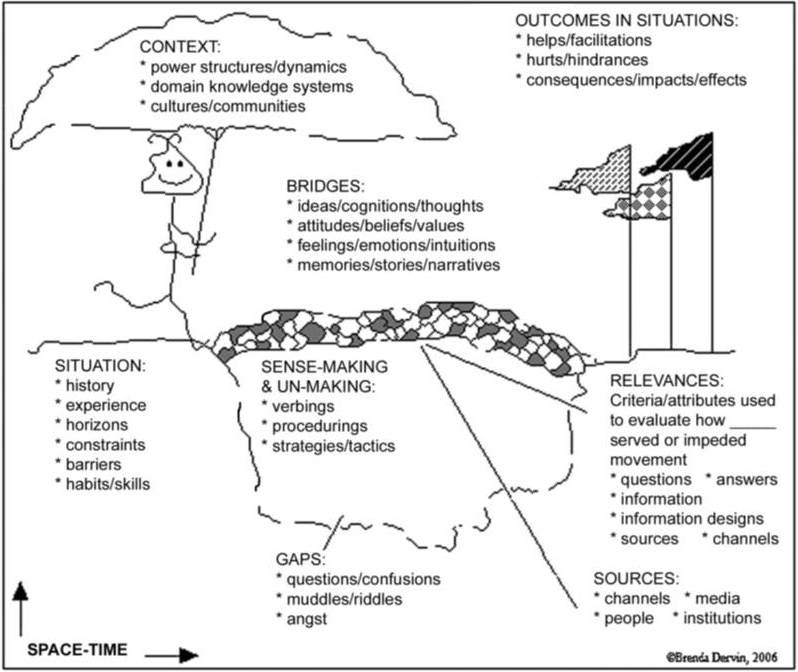
\includegraphics[width=\columnwidth]{dervin}
	\caption{The gap-bridging metaphor of sensemaking. People encounter gaps when moving through time-space, then seek for information, evaluate and use it to bridge the gaps. \is{Dervin2012}}
	\label{fig:lr-dervin}
\end{figure}

Dervin also implements the theory into a set of questions that can be used in interview to understand sensemaking within a context~\cite{Dervin1983}. The questions elaborate all parts of the model, aiming to establish an understanding on the situation (\emph{What happened?}), the gap (\emph{What did you struggle with?}), the bridge (\emph{What idea did you come to?}) and the outcome (\emph{How did that help?}).

\subsection{Learning Loop Complex}
In the context of human-computer interaction, Russell~et~al.~\cite{Russell1993} defines sensemaking as the process of searching for a representation and encoding data in that representation to answer task-specific questions. That cyclic process is called the \emph{learning loop complex} as illustrated in \autoref{fig:lr-russell}. First, the sensemaker searches for a representation to capture salient features of the data (\emph{Generation Loop}). During sensemaking, new information is sought and encoded into this representation (\emph{Data Coverage Loop}). The data unfit to the representation (\emph{residue}) requires the sensemaker to adjusts and produces a more suitable one. This entire learning loop complex is guided by the task with an aim to reduce its cost.

\begin{figure}[!htb]
	\centering
	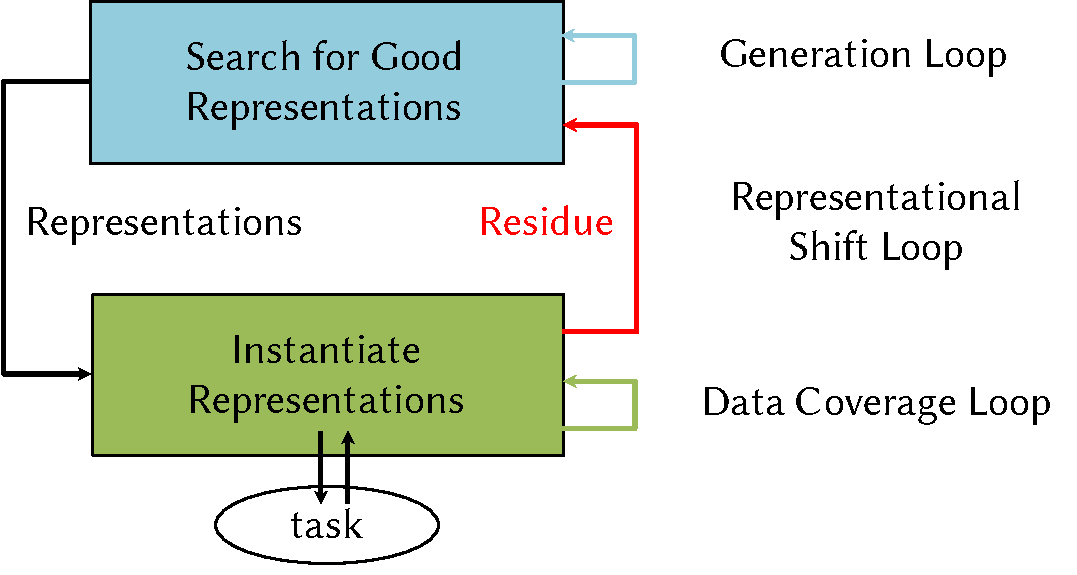
\includegraphics{russell}
	\caption{The learning loop complex theory of sensemaking. It consists of three iterative loops: searching for a good representation, encoding data to the representation, and adjusting the representation for a better data coverage. \is{Russell1993}}
	\label{fig:lr-russell}
\end{figure}

\subsection{Sensemaking in Organizations}
Different from Dervin and Russell who study sensemaking for individuals, Weick focuses on sensemaking at an organization level~\cite{Weick1995}. He proposes that sensemaking consists of these seven following properties.

\begin{enumerate}
	\item \emph{Grounded in identity construction}. Who people think they are, both individually and collectively, affect what they interpret and act.
	\item \emph{Retrospective}. People look back and make sense from what they have said and what they have done before.
	\item \emph{Enactive of sensible environments}. People make sense and contribute to the environments during their sensemaking processes.
	\item \emph{Social}. This is an inherent property of sensemaking in organization where people interact and socialize with others, and also are influenced by others.
	\item \emph{Ongoing}. Sensemaking is a continuous flow because the world and our understanding about the word are constantly changing.
	\item \emph{Focused on and by extracted cues}. Cues are things from the context that people have attention to and may use them to guide further exploration and assessment of the sensemaking problem.
	\item \emph{Driven by plausibility rather than accuracy}. Sensemaking is about plausibility and sufficiency rather than accuracy and completeness. People tend to stop searching when they find an acceptable solution.
\end{enumerate}

\subsection{A Process Model}
\label{sub:lr-pcm}
Pirolli and Card~\cite{Pirolli2005} describe sensemaking as an iterative process that gradually transforms raw data into rational knowledge. The process includes two sets of activities: one that cycles around finding relevant information, and another that cycles around making sense of that information, with plenty of interaction between them. They map to the \emph{foraging loop} and the \emph{sensemaking loop} respectively, as shown in \autoref{fig:lr-pirolli-card-model}. The sensemaking process can progress upward (from data to knowledge) or downward (from knowledge to data). The steps in the \emph{bottom-up} process are summarized as follows.

\begin{figure}[!htb]
	\centering
	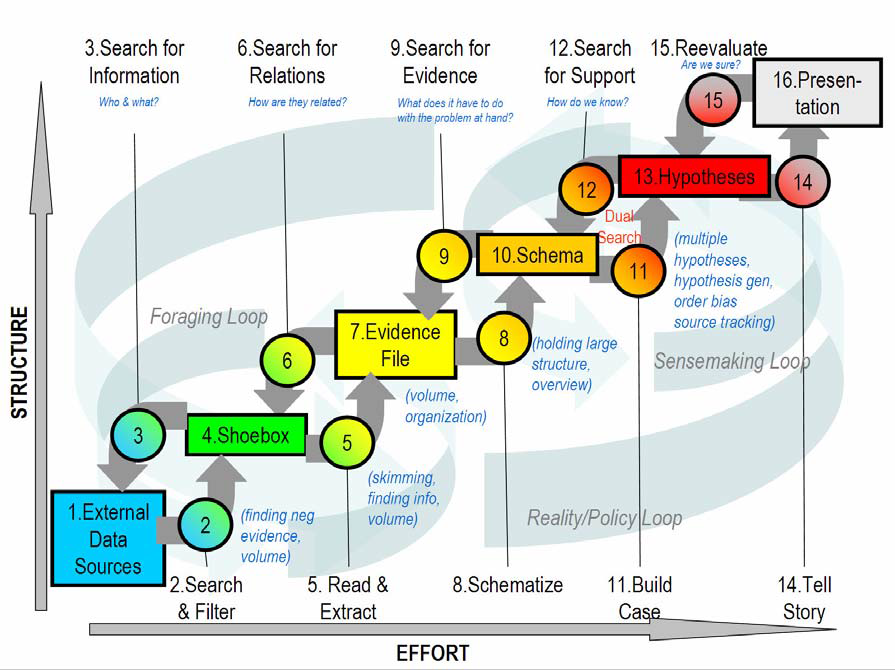
\includegraphics[width=\columnwidth]{pirolli-card-model}
	\caption{A notional model of sensemaking. The sub-processes (numbered circles) and their data input/output (numbered rectangles) are arranged in a two-dimensional space, in which the horizontal axis represents the degree of effort from users, and the vertical axis represents the degree of structure in information representation. \is{Pirolli2005}}
	\label{fig:lr-pirolli-card-model}
\end{figure}

\begin{itemize}
	\item \emph{Search and filter}. External data sources, such as classified databases or the web, are searched and filtered to retrieve relevant documents to the task.
	\item \emph{Read and extract}. These documents are examined to extract pieces of information that may be used as evidence later.
	\item \emph{Schematize}.  The collected information is organized in a way that aids the analysis. This may be executed in user mind, using paper and pen, or with a complex computer-based system.
	\item \emph{Build case}. Multiple hypotheses are generated; evidence are marshaled to support or disconfirm them.
	\item \emph{Tell story}. Discovered cases are presented to some audience.
\end{itemize}

In this model, \emph{schematization} plays an important role in converting raw evidence to rational explanations, bridging the foraging and sensemaking loops. A study by Kang, Görg and John Stasko~\cite{Kang2011} agrees with this observation. In their study, all the participants who performed the sensemaking task well spent considerable time and effort in organizing their collected information. Their organizational schemes were flexible: a \emph{timeline} of related events, a \emph{map} connecting locations that a person has been to, and a \emph{diagram} showing relationships among suspicious targets.

\subsection{Data--Frame Model}
\label{sub:lr-dfm}
Klein et al.~\cite{Klein2003} propose a sensemaking model that centers around \emph{data} and \emph{frame}. Data is the information that a person receives or searches for, and frame is the mental structure that organizes and explains the relationship of such data. For instance, a frame can be a \emph{story}, explaining the chronology of events and the causal relationships between
them; or a \emph{map}, showing where the events take place and the routes between them. Sensemaking is considered as a deliberate effort to understand an event, starting when a person realizes a gap of their current understanding of that event. Klein and his associates describe seven activities involved in sensemaking and are summarized in \autoref{fig:lr-data-frame-model}.

\begin{figure}[!htb]
	\centering
	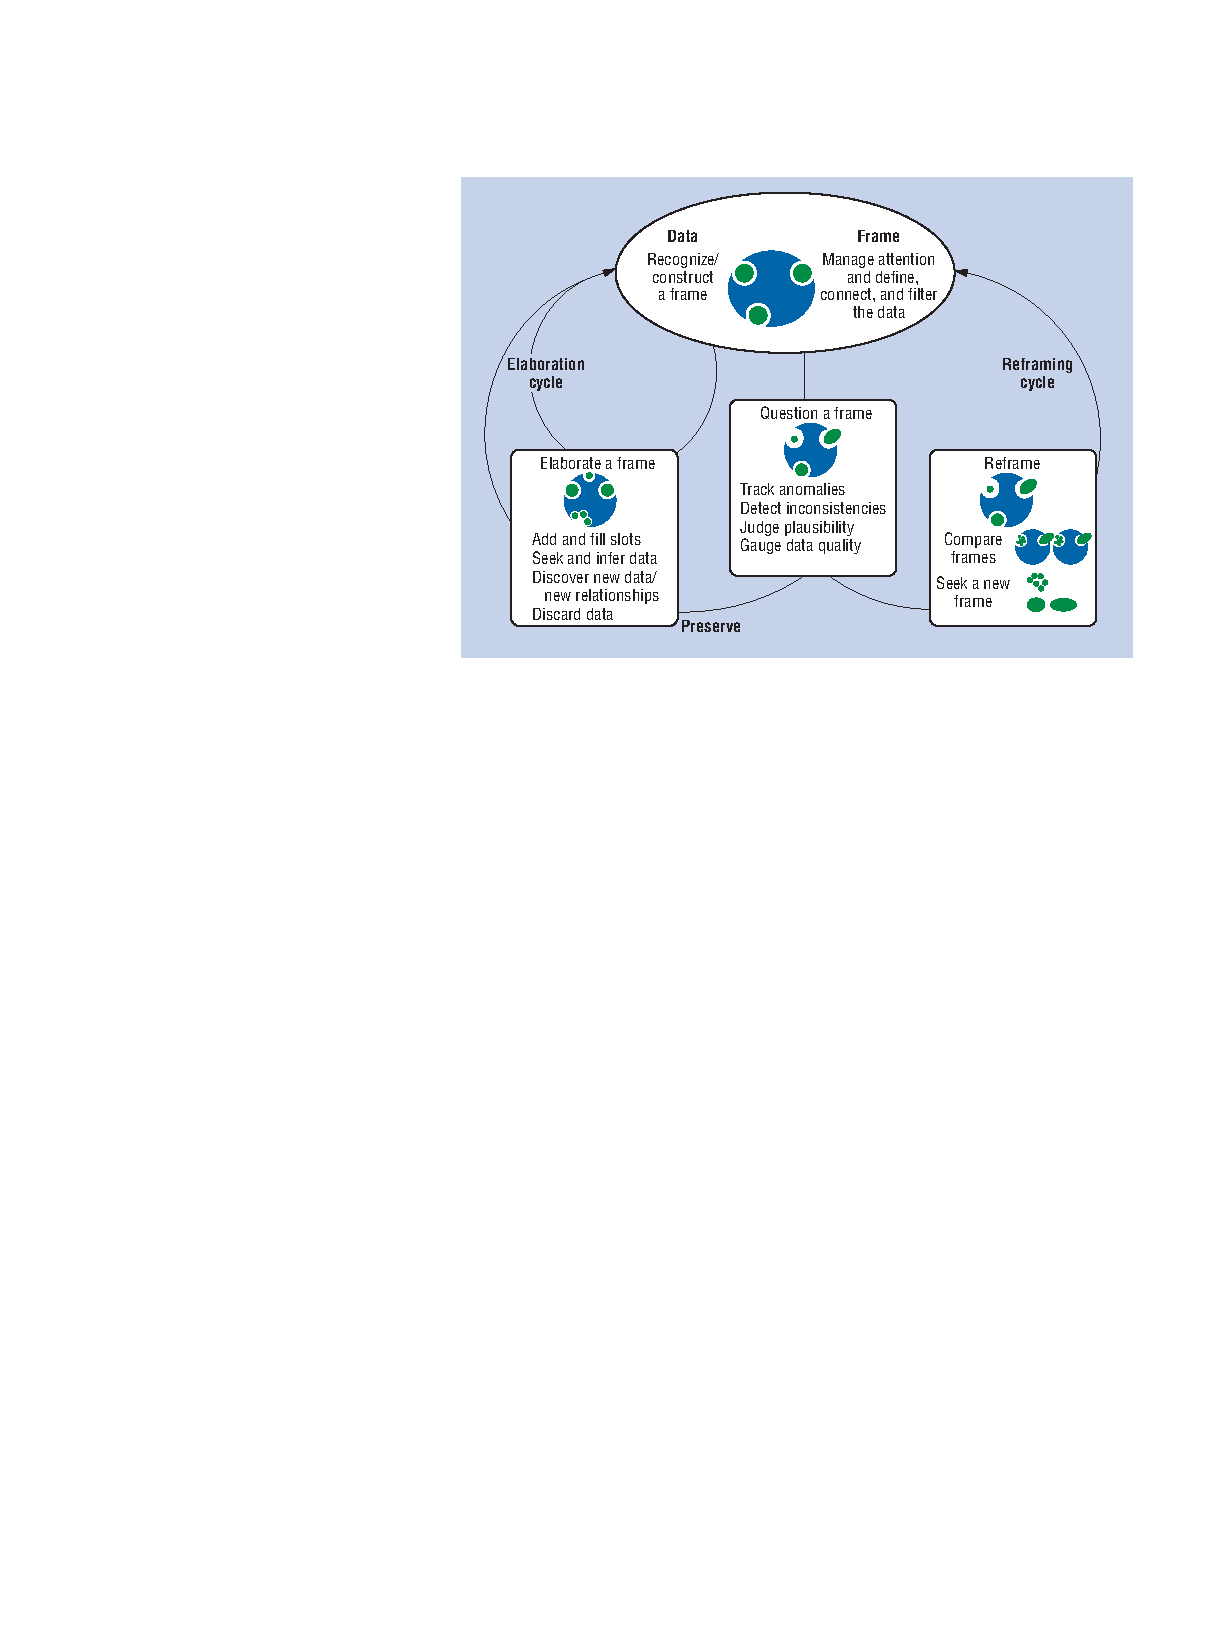
\includegraphics[width=\columnwidth]{data-frame-model}
	\caption{The data--frame model of sensemaking. It describes a set of interconnected sensemaking activities centering around data and frame -- the explanatory structure of data. \is{Klein2003}}
	\label{fig:lr-data-frame-model}
\end{figure}

\begin{itemize}
	\item \emph{Connect data and a frame}. A person recognizes relevant pieces of data and constructs an initial frame to explain them. The frame then helps the person to filter and search for new data.
	\item \emph{Elaborate the frame}. As more is learned about the situation, the frame becomes more elaborate with new data and new relationships. 
	\item \emph{Question the frame}. It happens when a person encounters data that is inconsistent with the existing frame. At this point, the person may be unsure that the frame is incorrect, or the inconsistent data is inaccurate.
	\item \emph{Preserve the frame}. A person may consider the severity of the inconsistent data, justify why it mismatches the frame, and ignore it.
	\item \emph{Compare multiple frames}. Depending on experience, a person may think of alternative frames explaining the same set of data. These frames need to be compared to select the most likely one.
	\item \emph{Reframe}. When encountering inconsistent and contrary data, the person may need to find a replacement that can explain all data. Considering discarded data and/or reinterpreting data could facilitate this activity.
	\item \emph{Seek a new frame}. A person may deliberately search for a new frame when encountering plenty of conflicted data. One or two key data elements may serve as \emph{anchors} to help the person to elicit another frame.
\end{itemize}

The Pirolli and Card's model describes a step-by-step process of sensemaking, in which the analyst collects relevant data and eventually transposes it into rational answers. However, the various sensemaking activities in the Data--Frame model may explain the strategies used by the analyst more comprehensively.

TODO: summary
A recent and comprehensive review of sensemaking can be found in the article by Maitlis and Christianson~\cite{Maitlis2014}.
%\section{Visualization and Visual Analytics}

\subsection{Overview}
Computer-based visualization systems provide visual representations of datasets designed to help people carry out tasks more effectively~\cite{Munzner2014}. Because the design space of possible visual ``idioms'' is huge, it is challenging to create effective visualizations. Understanding well-established information design principles and interaction techniques could guide designers toward the right direction. Also, every visualization needs to be evaluated to check whether it meets its design purposes and how it helps or hinder users.

Overview: what is vis? what can vis help? what is VA? what can VA help, in addition to vis? explain the VA process model. briefly explain the 3 important blocks in the model, which are then discussed in detail next. 

%What is vis? Classic example. What vis can help from cognition (Ben) and Wijk, Fekete?
%
%Large datasets -> simple aggregation, reduction like filtering, interaction, ; larger datasets, more sophiscated emthods extract patterns and vis to display them. and allow further. That is the idea of visual analytics. Orginal def, new def. Model.
%
%Describe visual analytics process model (Figure~\ref{fig:visual-analytics-process})
%
%\begin{figure}[!htb]
%	\centering
%	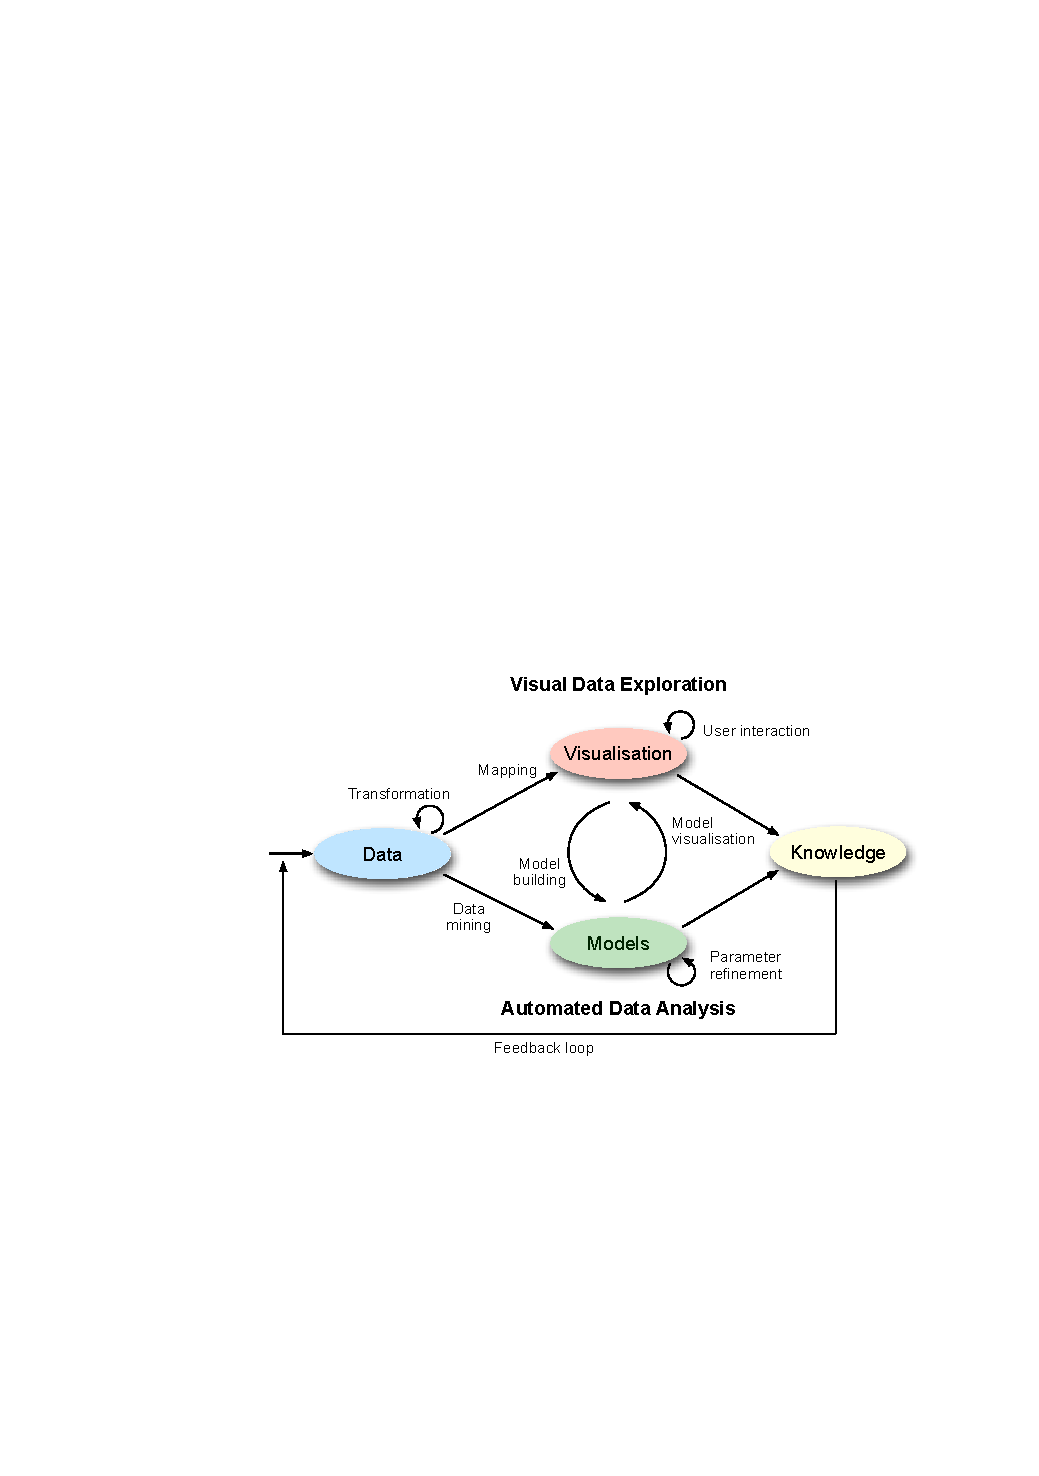
\includegraphics[width=\columnwidth]{visual-analytics-process}
%	\caption{The visual analytics process model. \emph{Source:~\cite{Keim2010}}.}
%	\label{fig:visual-analytics-process}
%\end{figure}
%
%
%Next, discuss basics of vis and models. and evaluation.

\subsection{Visualization Design}


\subsubsection{Information Design Principles}
\label{sub:lr-design}

\paragraph{Marks and Channels}
Marks are basic geometric elements that depict items or links, and channels control their appearance~\cite{Munzner2014}. Item marks can be zero-dimensional as a \emph{point}, one-dimensional as a \emph{line}, two-dimensional as an \emph{area}, and three-dimensional as a \emph{volume}, but rarely used. Link marks include \emph{connection} showing a pairwise relationship between two items using a line and \emph{containment} showing hierarchical relationships using areas. \autoref{fig:lr-marks} illustrates these marks. 

\begin{figure}[!htb]
	\centering
	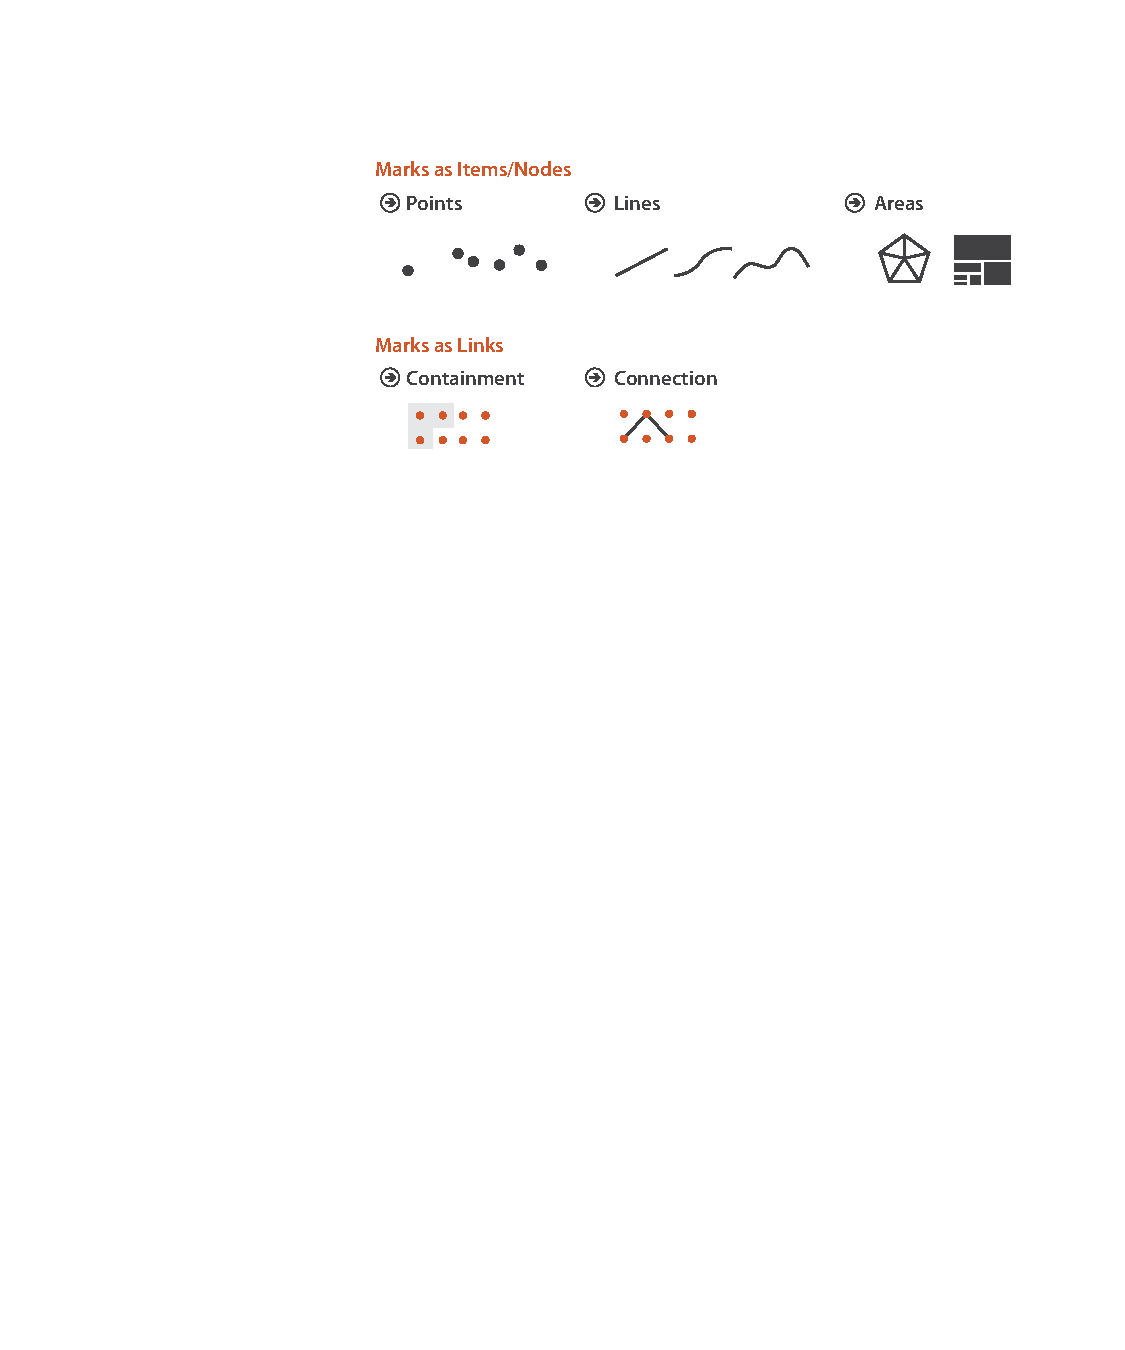
\includegraphics[width=.8\linewidth]{marks}
	\caption{Item and link marks as geometric primitives. \is{Munzner2014}}
	\label{fig:lr-marks}
\end{figure}

A visual channel control the appearance of marks, independent of their dimensionality. Examples include position, color, shape, angle and size. However, not all channels can be applied to all marks. For instance, an area mark is used in a geographic map to denote a region. It is already associated with a shape and size, thus cannot be size coded to represent another quantitative attribute.
some visual channels. some cannot encode size, example. \autoref{fig:lr-channel-example} shows a progression of chart types, with each showing one more data attribute using one more visual channel. \autoref{fig:lr-channel-example-1} shows a bar chart representing a single quantitative attribute using the \emph{vertical position} channel. \autoref{fig:lr-channel-example-2} shows a scatter plot encoding the second quantitative attribute using the \emph{horizontal position} channel. \autoref{fig:lr-channel-example-3} adds the \emph{color} channel to represent a categorical attribute, and \autoref{fig:lr-channel-example-4} adds the \emph{size} channel to represent another quantitative attribute. In these examples, each attribute is encoded with a single channel. However, multiple channels can be combined to redundantly encode the same attribute, helping perceive it more easily.

\begin{figure}[!htb]
\centering
\subcaptionbox{Line marks with horizontal position for a categorical attribute and vertical position for a quantitative attribute.\label{fig:lr-channel-example-1}}{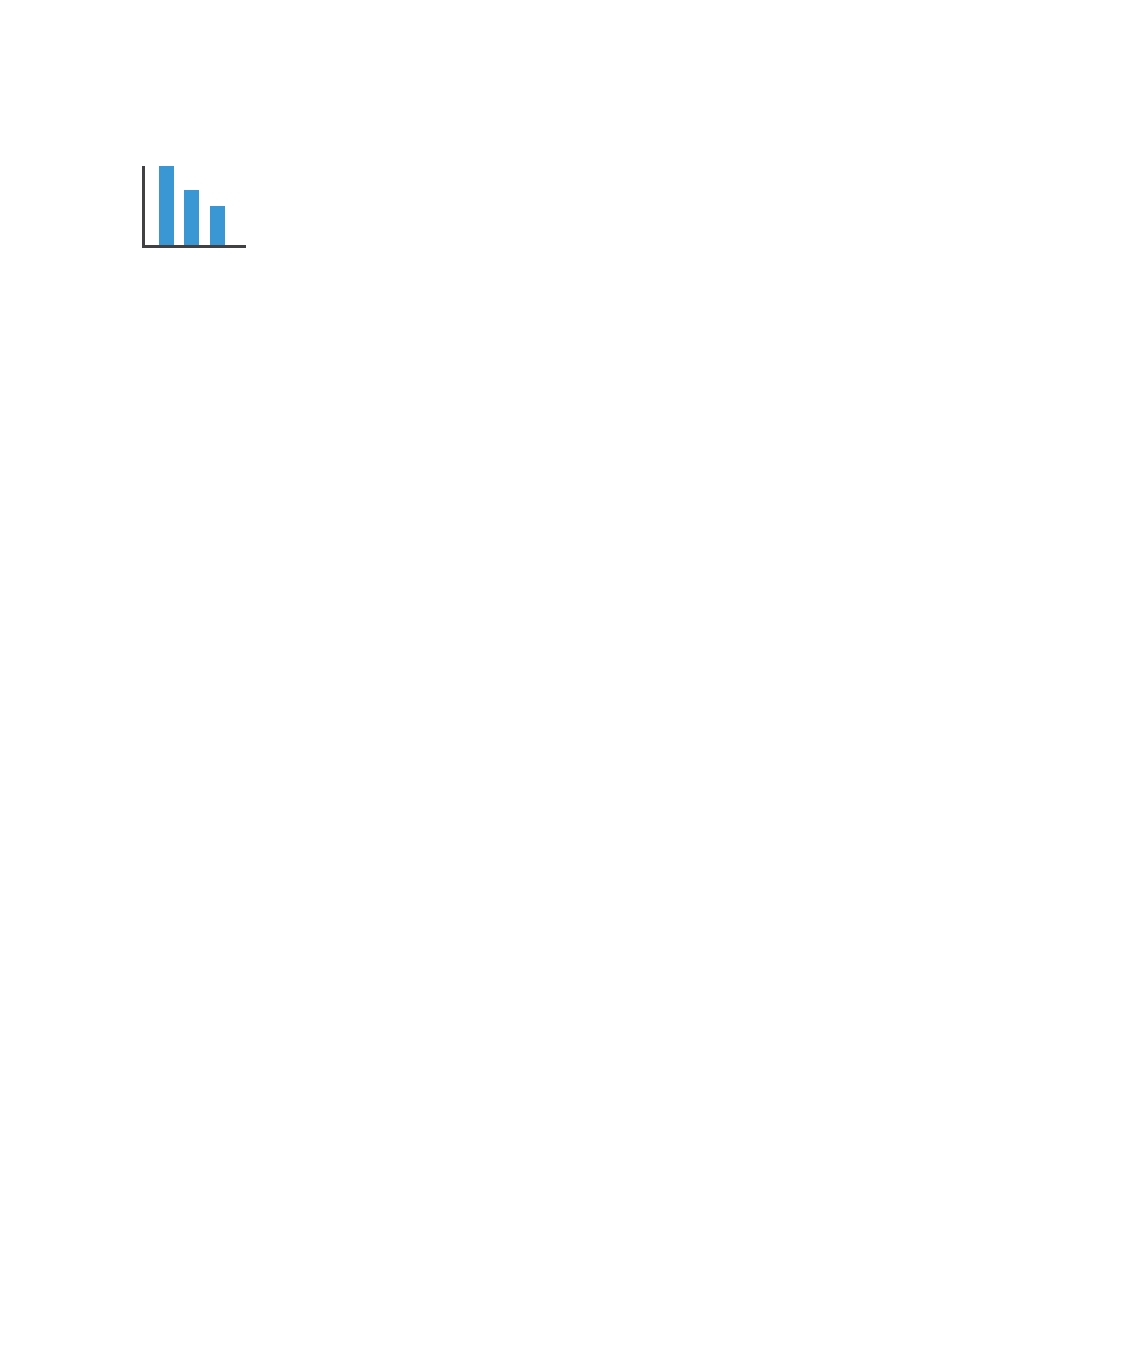
\includegraphics[width=.23\columnwidth]{channel-example-1}} 
\hfill
\subcaptionbox{Point marks with both horizontal and vertical position channels for quantitative attributes.\label{fig:lr-channel-example-2}}{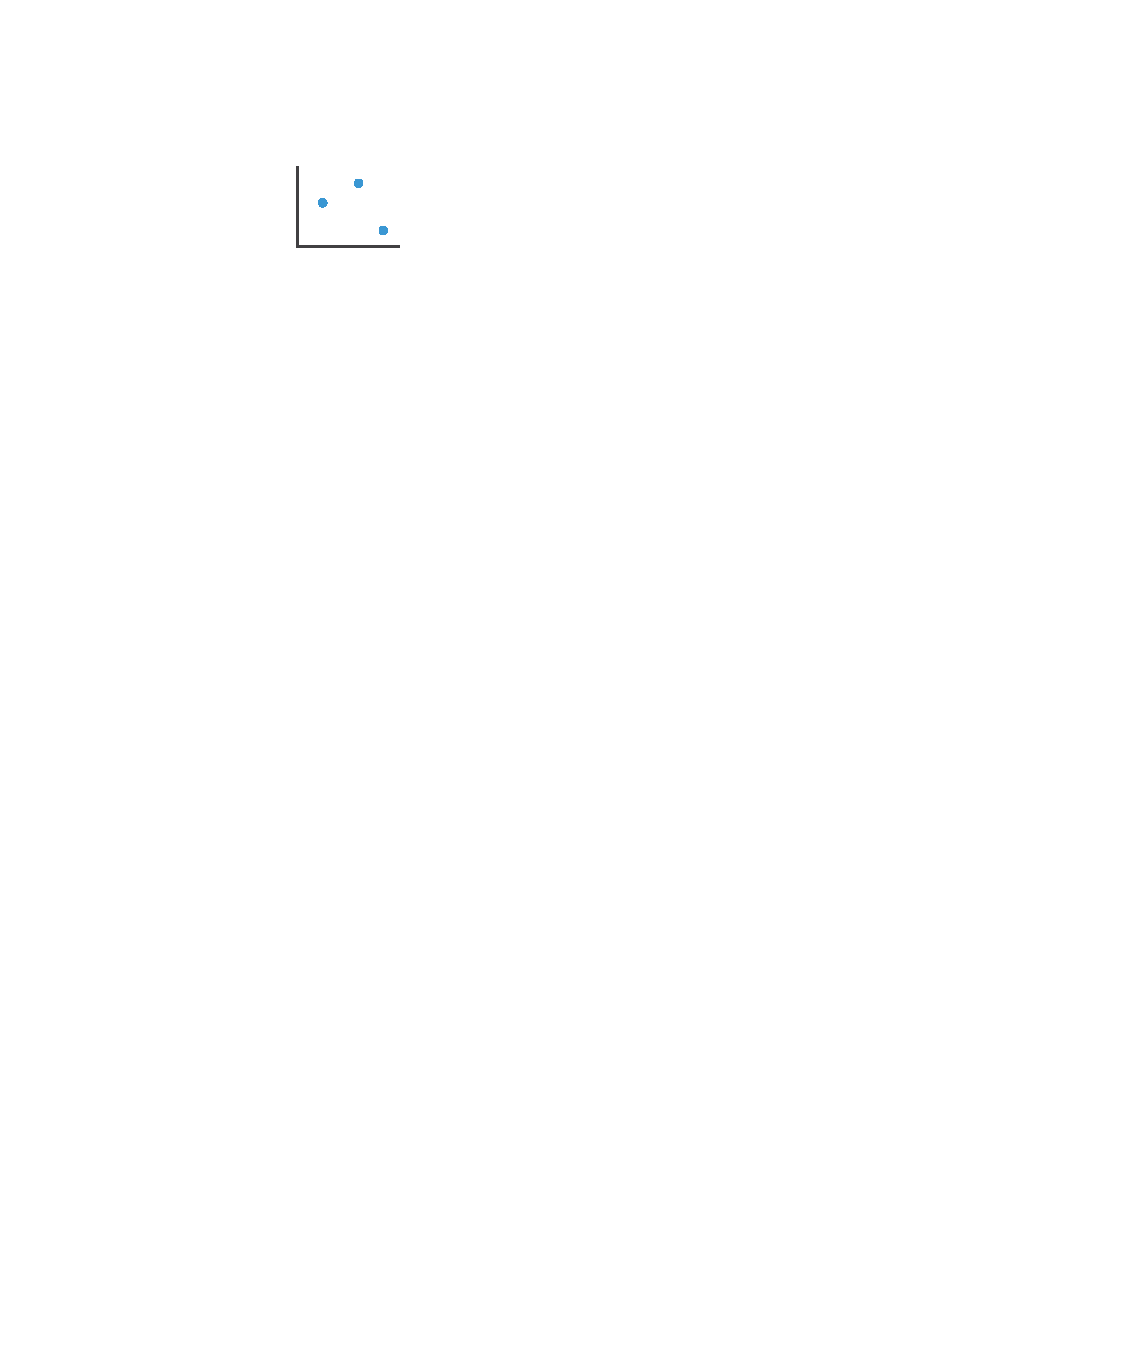
\includegraphics[width=.23\columnwidth]{channel-example-2}} 
\hfill
\subcaptionbox{A categorical attribute is added using the color channel.\label{fig:lr-channel-example-3}}{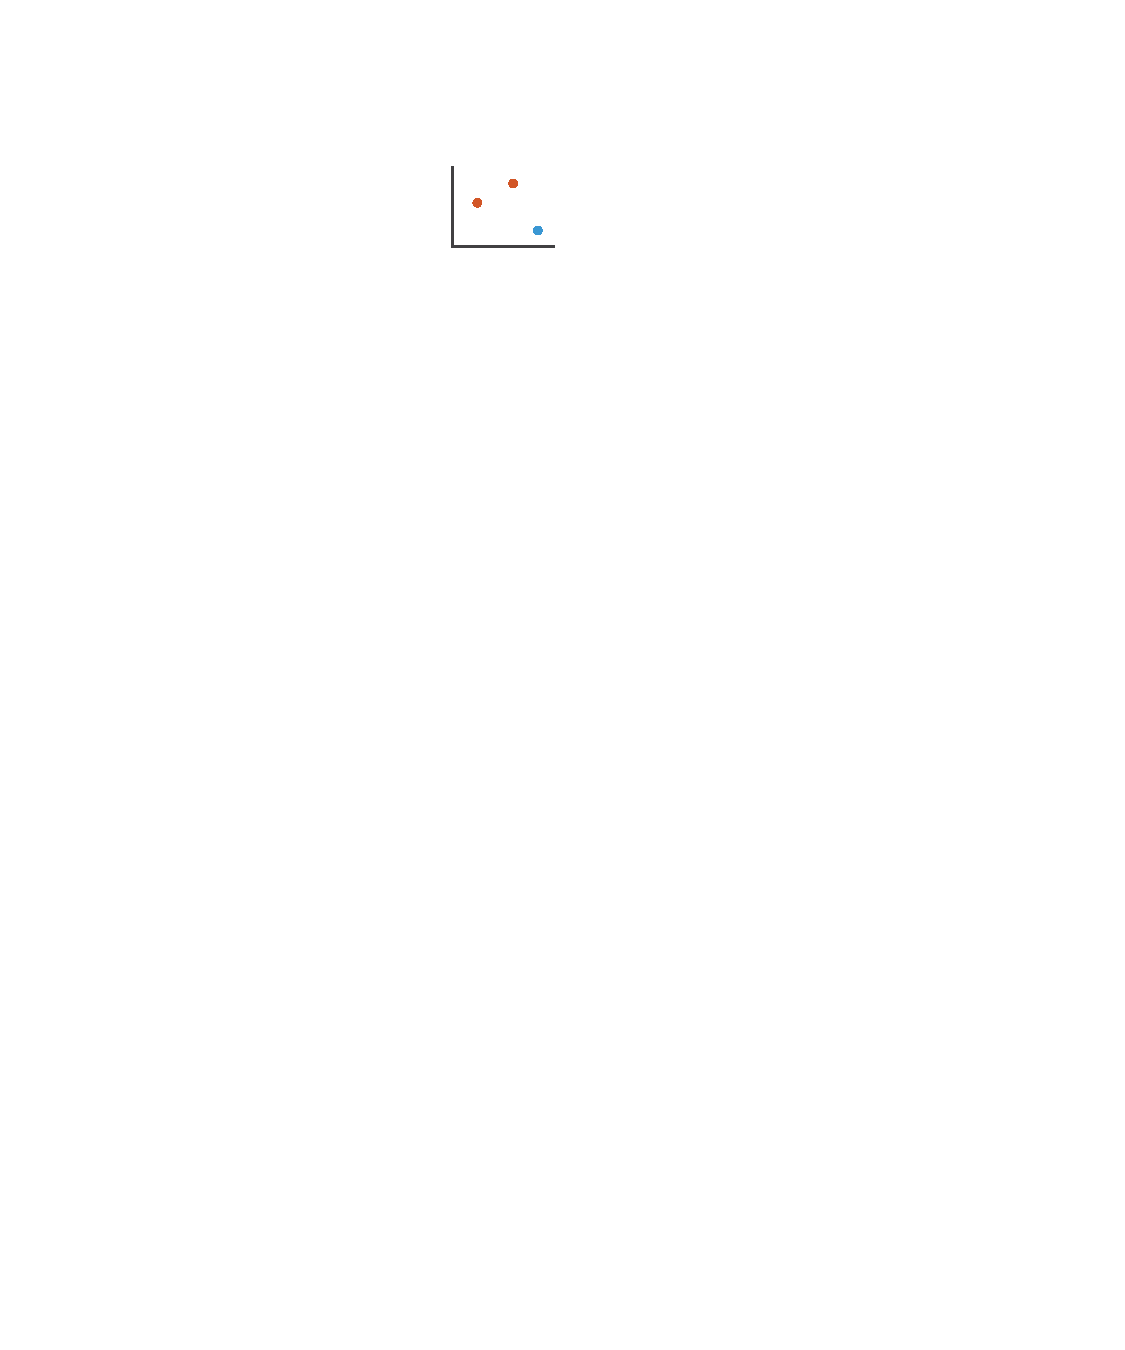
\includegraphics[width=.23\columnwidth]{channel-example-3}}
\hfill
\subcaptionbox{Another quantitative attribute is added using the size channel.\label{fig:lr-channel-example-4}}{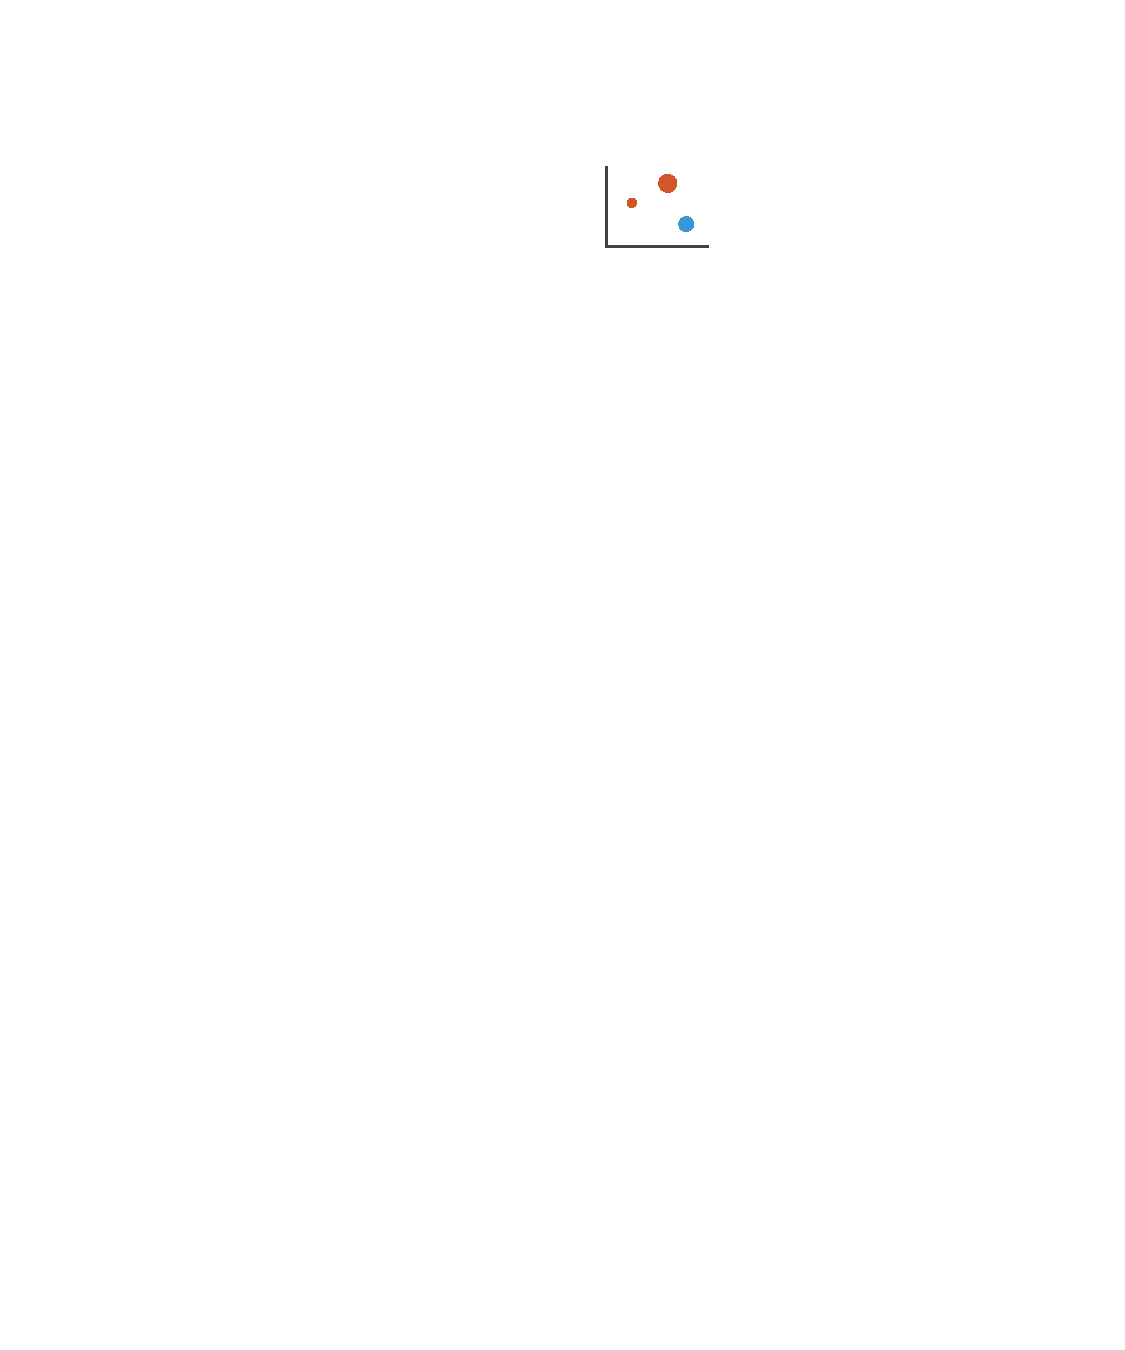
\includegraphics[width=.23\columnwidth]{channel-example-4}}
\caption{Using marks and channels.}
\label{fig:lr-channel-example}
\end{figure}

All channels are not equal; they are processed and perceived differently by our human visual systems. Also, not all channels are appropriate for encoding both ordered and categorical attributes. Ordered attributes should be shown using magnitude channels, with \emph{aligned spatial position} as the most effective channel and \emph{3D volume} as the least effective one. Categorical attributes should be shown using identity channels, with \emph{spatial region} as the most effective channel and \emph{shape} as the least effective one. \autoref{fig:lr-channel-ranking} shows the detailed ranking of effectiveness of many visual channels, separated by the type of attribute. This ranking is documented by Munzner~\cite{Munzner2014}, based on many empirical studies such as the work by Cleveland and McGill~\cite{Cleveland1985}, and by Heer and Bostock~\cite{Heer2010a}.

\begin{figure}[!htb]
	\centering
	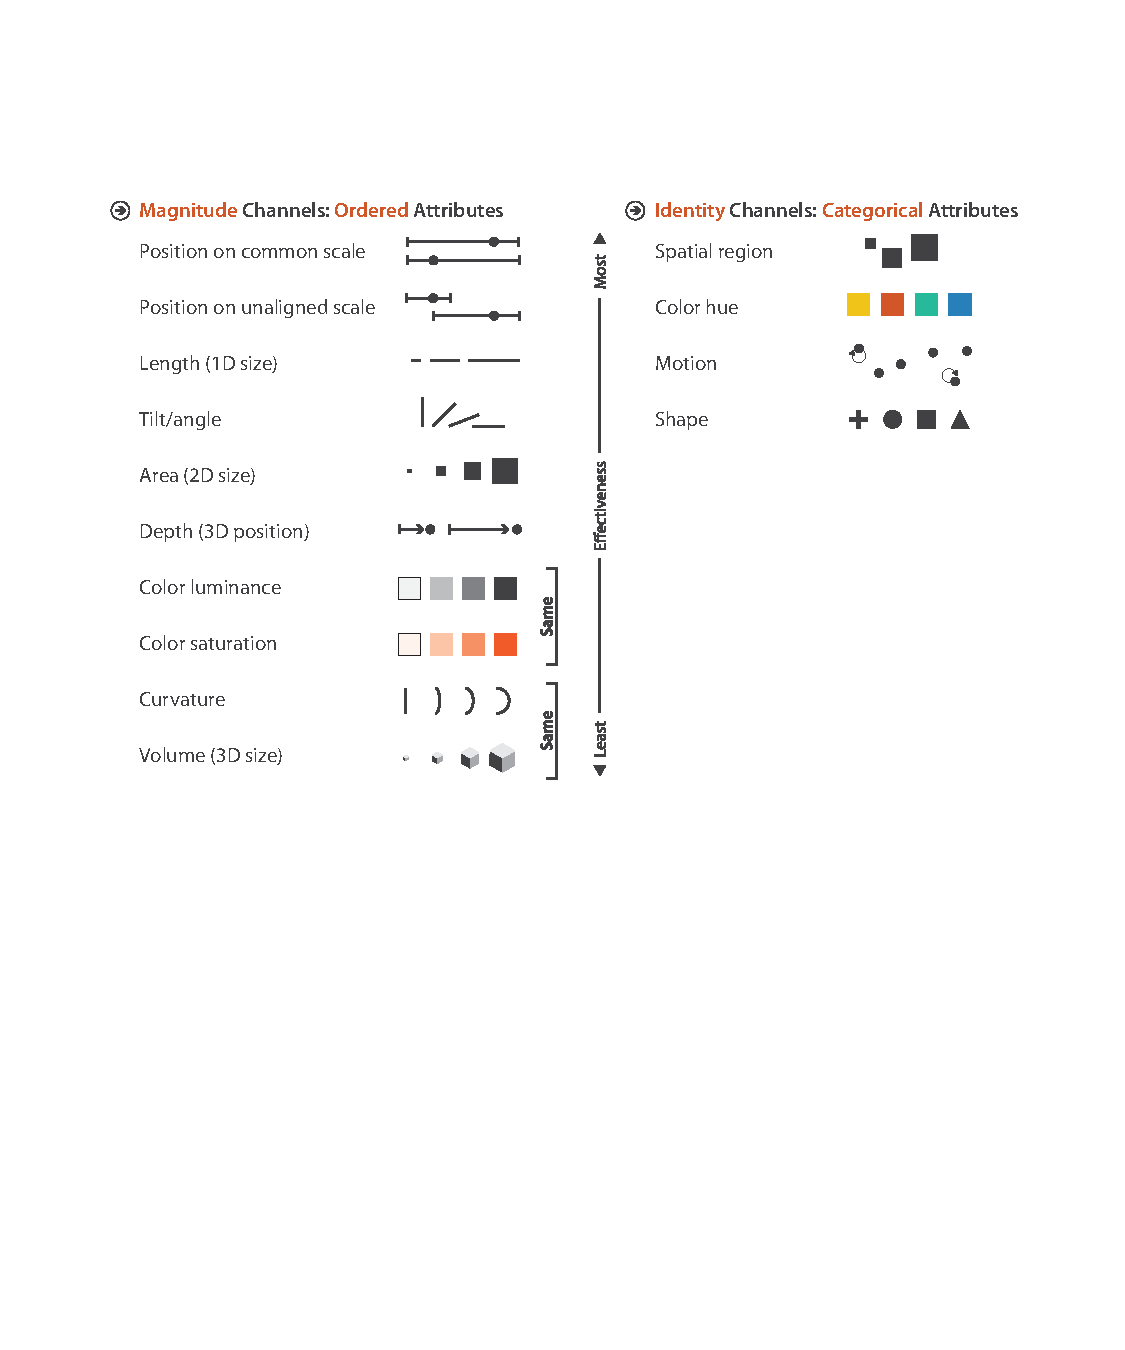
\includegraphics[width=\linewidth]{channel-ranking}
	\caption{Channels ranked by effectiveness according to data and channel type. \is{Munzner2014}}
	\label{fig:lr-channel-ranking}
\end{figure}

Color is a special channel that can be used for both data attributes. As shown in \autoref{fig:lr-channel-ranking}, color luminance and saturation are used in magnitude channels, and color hue is used in identity channels. A colormap specifies a mapping between colors and data values, and designing an effective colormap is challenging. ColorBrewer~\cite{Harrower2003} is an excellent source for colormap reference, providing color schemes for both categorical and ordered attributes. Human can only distinguish around 12 colors simultaneously~\cite{Munzner2014}. \autoref{fig:lr-colorbrewer-1} shows such a categorical colormap with 12 distinguished color hues. Ordered colormaps can be either sequential (\autoref{fig:lr-colorbrewer-2}) or diverging (\autoref{fig:lr-colorbrewer-3}). Diverging colormaps use two different color hues to emphasize values below and above the middle point.

\begin{figure}[!htb]
\centering
\subcaptionbox{Categorical colormap with distinguishable color hues.\label{fig:lr-colorbrewer-1}}[\columnwidth]{
\includegraphics[width=.6\columnwidth]{colorbrewer-1}} 
\\
\subcaptionbox{Sequential colormap: a single color hue with different saturation level.\label{fig:lr-colorbrewer-2}}[\columnwidth]{\hspace{-.15\columnwidth}
\includegraphics[width=.45\columnwidth]{colorbrewer-2}}
\\
\subcaptionbox{Diverging colormap: two color hues emphasizing positive and negative values.\label{fig:lr-colorbrewer-3}}[\columnwidth]{\hspace{-.05\columnwidth} 
\includegraphics[width=.55\columnwidth]{colorbrewer-3}}
\caption{Colormaps from ColorBrewer. \is{Harrower2003}}
\end{figure}

\subparagraph{Gestalt Principles}
\label{sub:lr-gestalt}
Gestalt principles describe how we see patterns in visual displays~\cite{Koffka1935}. This section reviews three commonly used principles in representing groups of items.

\subparagraph{Similarity} 
Similar elements tend to be grouped together. \autoref{fig:lr-gestalt-similarity-1} shows a matrix of point marks with uniform spacing, but using two different shapes: dot and cross. The similarity of shapes helps us see the rows more clearly than the columns. Two separable channels can be applied together to reveal patterns by either rows or columns. In \autoref{fig:lr-gestalt-similarity-2}, green is used to depict rows, and texture is used to depict columns.

\begin{figure}[!htb]
\centering
\subcaptionbox{Similarity of shapes distinguishes rows.\label{fig:lr-gestalt-similarity-1}}[.47\columnwidth]{
\includegraphics[height=.35\columnwidth]{gestalt-similarity-1}} 
\hfill
\subcaptionbox{Color and texture delineate rows and columns, respectively.\label{fig:lr-gestalt-similarity-2}}[.47\columnwidth]{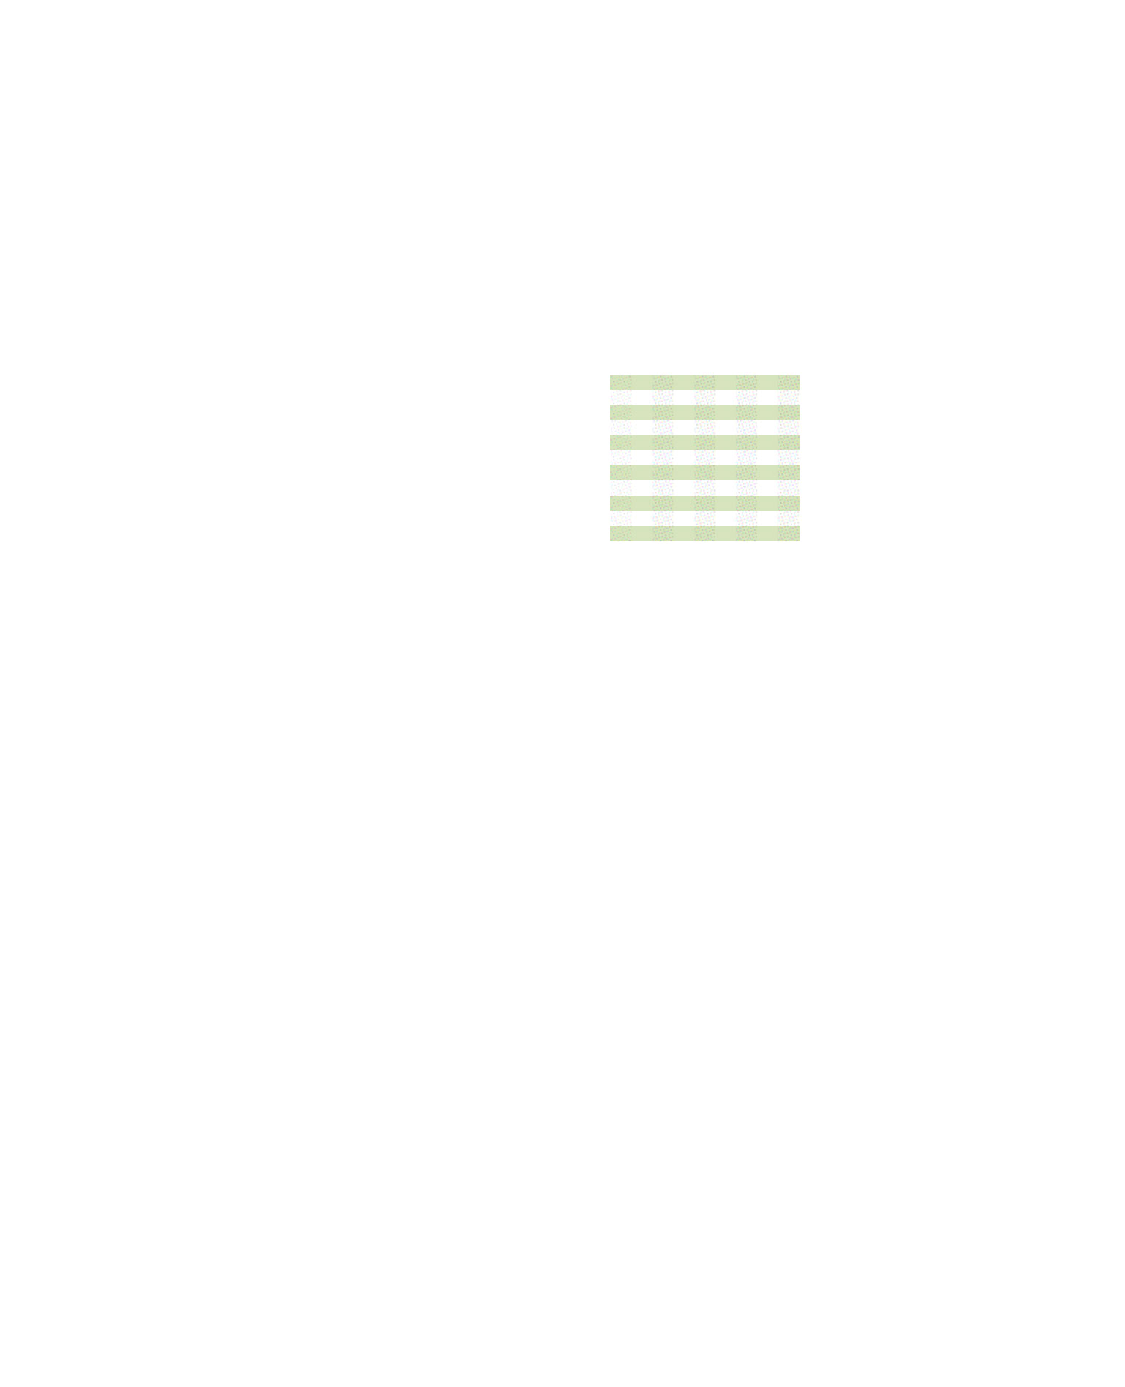
\includegraphics[height=.35\columnwidth]{gestalt-similarity-2}} \label{fig:lr-gestalt-similarity}
\caption{Similarity principle: similar elements are perceived as a group. \is{Ware2013}}
\end{figure}

\subparagraph{Proximity} 
Elements that are close together are perceptually grouped together. \autoref{fig:lr-gestalt-proximity-1} clearly shows two groups of dots. \autoref{fig:lr-gestalt-proximity-2} shows rows of dots. However, with a small change of spacing, these dots are perceived as columns in \autoref{fig:lr-gestalt-proximity-3}. The application of this principle is straightforward: organizing related information close together. It helps separate groups of unrelated objects and facilitates searching for information.

\begin{figure}[!htb]
\centering
\subcaptionbox{Two groups of dots.\label{fig:lr-gestalt-proximity-1}}{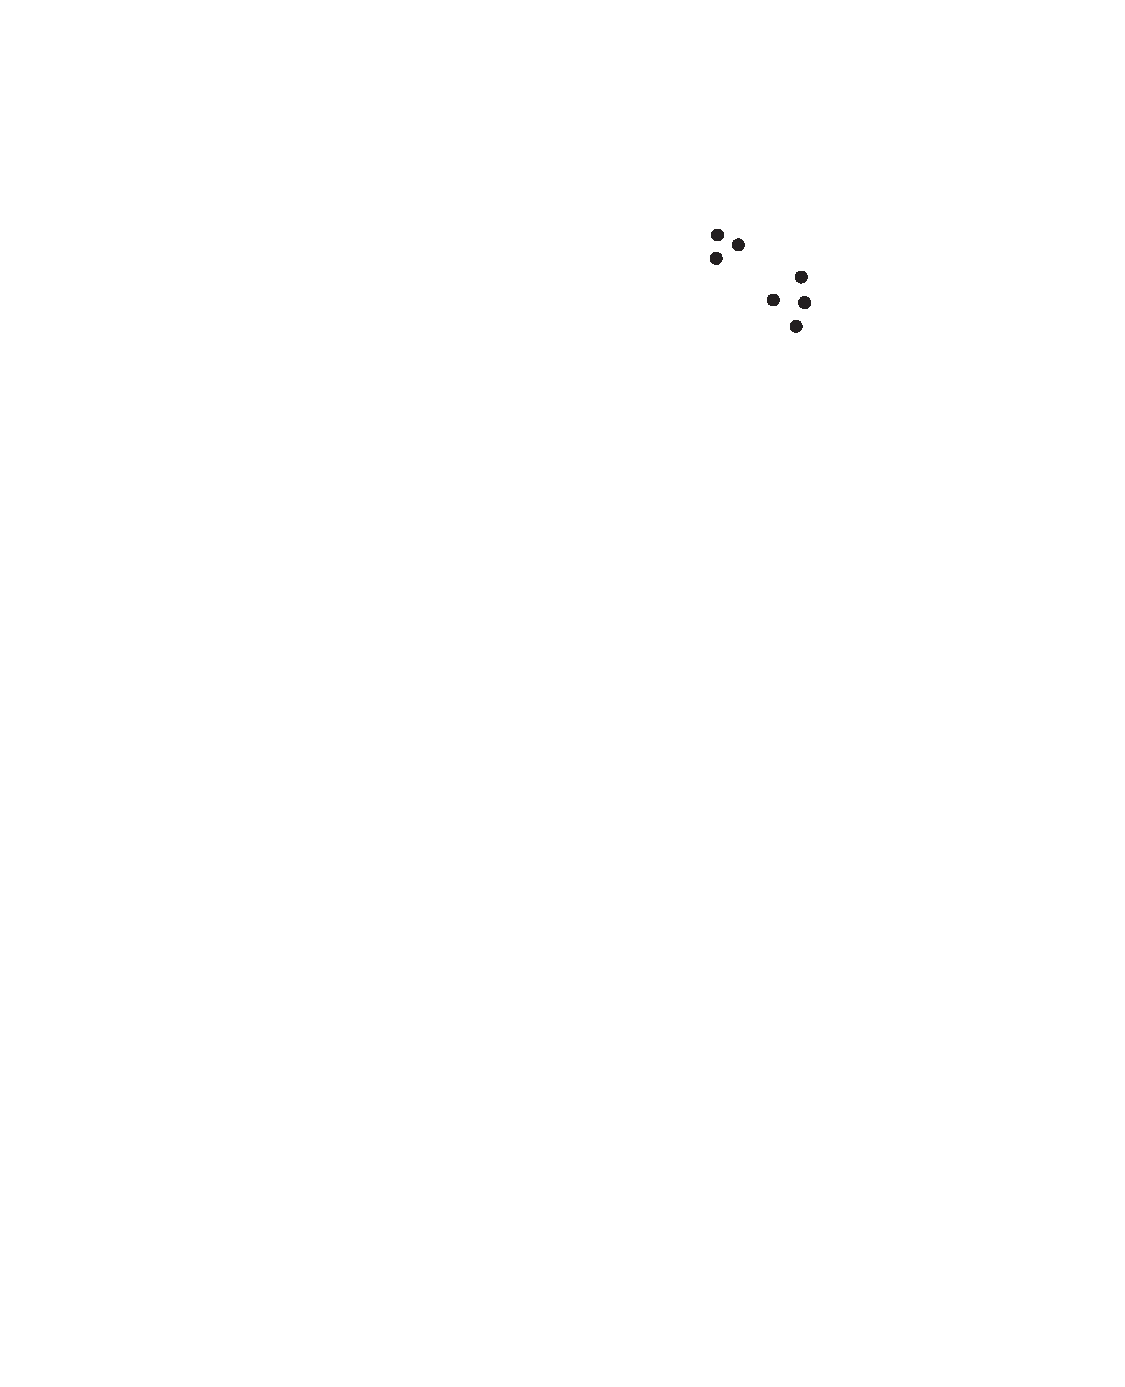
\includegraphics[width=.25\columnwidth]{gestalt-proximity-1}} 
\hfill
\subcaptionbox{Rows of dots.\label{fig:lr-gestalt-proximity-2}}{
\includegraphics[width=.31\columnwidth]{gestalt-proximity-2}} 
\hfill
\subcaptionbox{Columns of dots.\label{fig:lr-gestalt-proximity-3}}{
\includegraphics[width=.31\columnwidth]{gestalt-proximity-3}}
\label{fig:lr-gestalt-proximity}
\caption{Spatial proximity principle: spatially close elements are perceived as a group. \is{Ware2013}}
\end{figure}

\paragraph{Connectedness} 
Elements that are connected by visual properties are perceived as being more related than elements that are not connected. This principle can be achieved simply by drawing a border around a group of elements as in \autoref{fig:lr-gestalt-connectedness-1}. This is extensively applied in designing complex graphical user interface: groups of related features are separated by borders. Another approach to implement connectedness is by drawing lines between related elements as in \autoref{fig:lr-gestalt-connectedness-2}. This is the basics of \emph{node-link diagrams} -- one of the most common methods of representing relationships between elements.

\begin{figure}[!htb]
\centering
\subcaptionbox{Using border to denote a group.\label{fig:lr-gestalt-connectedness-1}}{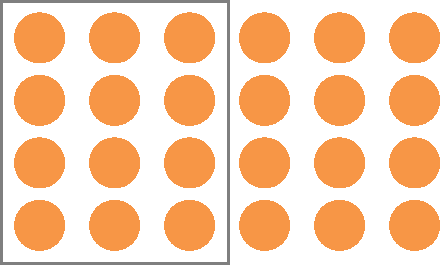
\includegraphics[width=.4\columnwidth]{gestalt-connectedness-1}} 
\hfill
\subcaptionbox{Using lines to denote a group.\label{fig:lr-gestalt-connectedness-2}}{
\includegraphics[width=.4\columnwidth]{gestalt-connectedness-2}} 
\caption{Connectedness principle: visually connected elements are perceived as a group. \is{Ware2013}}
\label{fig:lr-gestalt-connectedness}
\end{figure}

Among these three Gestalt principles of representing groups of elements, connectedness has the strongest effect, followed by proximity and then similarity. \autoref{fig:lr-gestalt} illustrates this comparison. In \autoref{fig:lr-gestalt-1}, even though spacing between dots in rows is shorter than spacing between dots in columns, the lines make the vertical links clearer than rows. In \autoref{fig:lr-gestalt-2}, the lines also make the horizontal links more notable than groups of colored circles. In \autoref{fig:lr-gestalt-3}, two spatial groups are more clearly perceived than colored groups.

\begin{figure}[!htb]
\centering
\subcaptionbox{Links are more clearly perceived than spatial groups.\label{fig:lr-gestalt-1}}[.3\columnwidth]{
\includegraphics[height=.12\columnwidth]{gestalt-1}} 
\hfill
\subcaptionbox{Links are more clearly perceived than colored groups.\label{fig:lr-gestalt-2}}[.3\columnwidth]{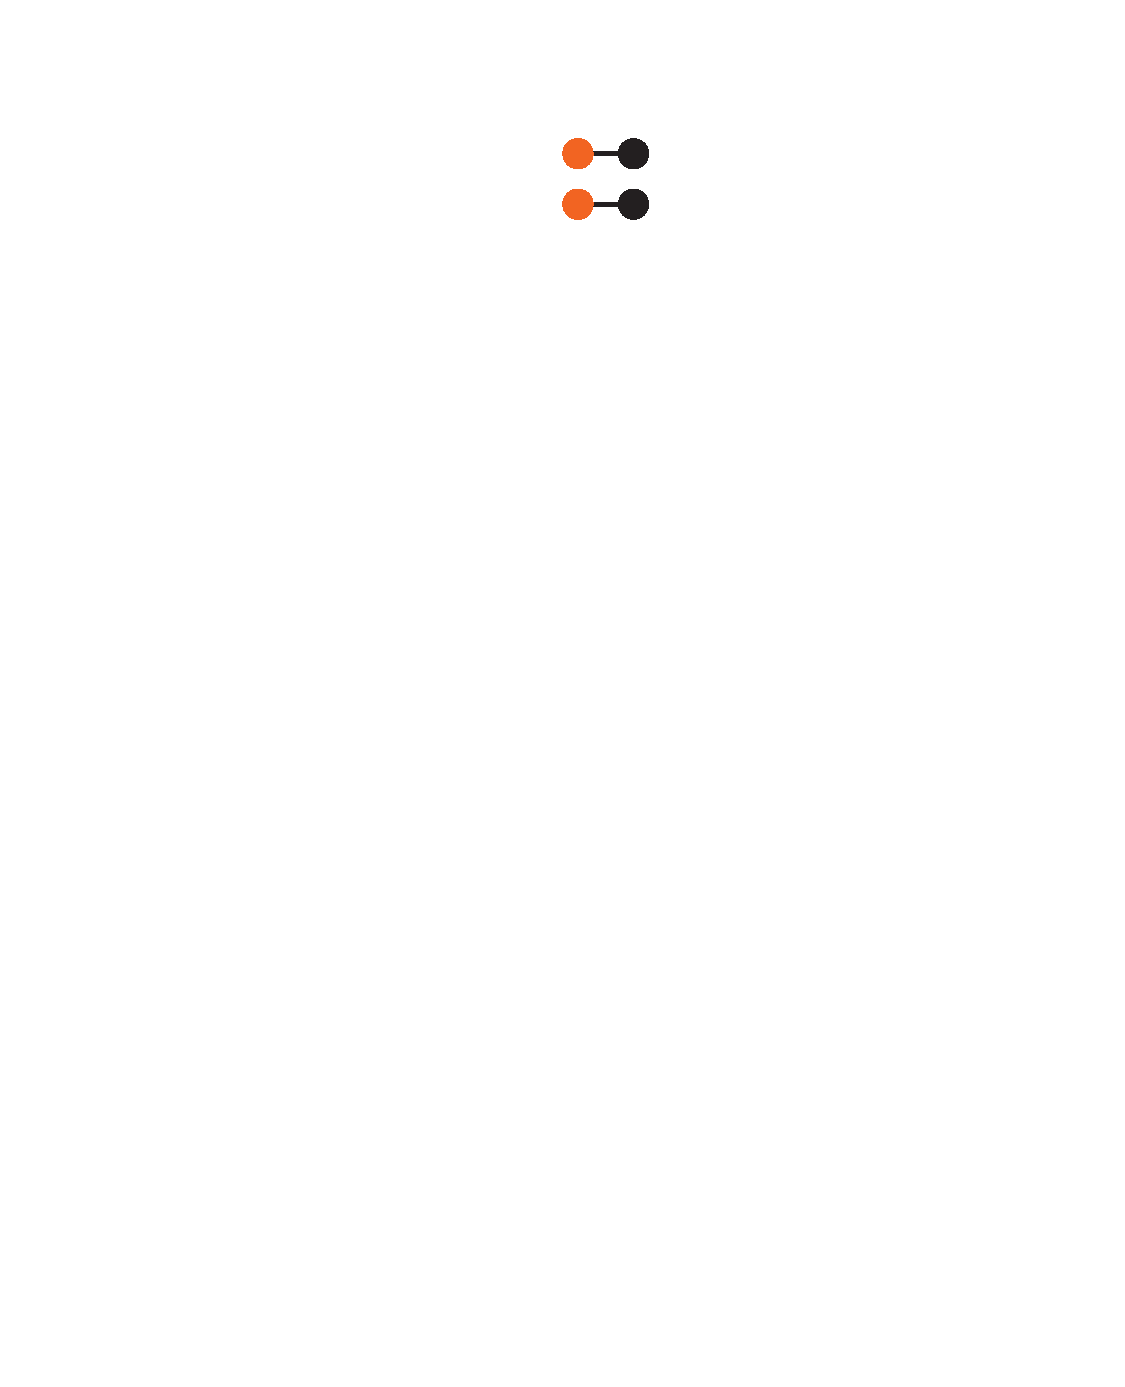
\includegraphics[height=.12\columnwidth]{gestalt-2}} 
\hfill
\subcaptionbox{Spatial groups are more clearly perceived than colored groups.\label{fig:lr-gestalt-3}}[.3\columnwidth]{
\includegraphics[height=.12\columnwidth]{gestalt-3}}
\caption{Comparison of Gestalt principles. Connectedness is stronger than proximity, and proximity is stronger than similarity. \is{Ware2013}}
\label{fig:lr-gestalt}
\end{figure}

\paragraph{Tufte's Principles}
Tufte proposes a number of principles for a well-designed graphic, documented in his series of books, most notably including \emph{The Visual Display of Quantitative Information}~\cite{Tufte1983} and \emph{Envisioning Information}~\cite{Tufte1990}. This section reviews a few principles that have been commonly applied in graphic design and visualization.

\subparagraph{Graphical Integrity}
This principle emphasizes that the graphical representation should tell the truth about the data. Representation of numbers, as physically measured on the surface of the	graphic	itself,	must be directly proportional to the numerical quantities represented~\cite{Tufte1983}. \autoref{fig:lr-tufte-integrity-1} shows a falsely big drop in stock market value between 2001 and 2002. It because the chart uses a relative scale with the value range from 450 to 500, causing its height disproportional to the market value. \autoref{fig:lr-tufte-integrity-2} corrects this error by using an absolute scale with the value range starting from 0.

\begin{figure}[!htb]
\centering
\subcaptionbox{Using a relative value range causes a falsely big drop of stock market value between 2001 and 2002.\label{fig:lr-tufte-integrity-1}}{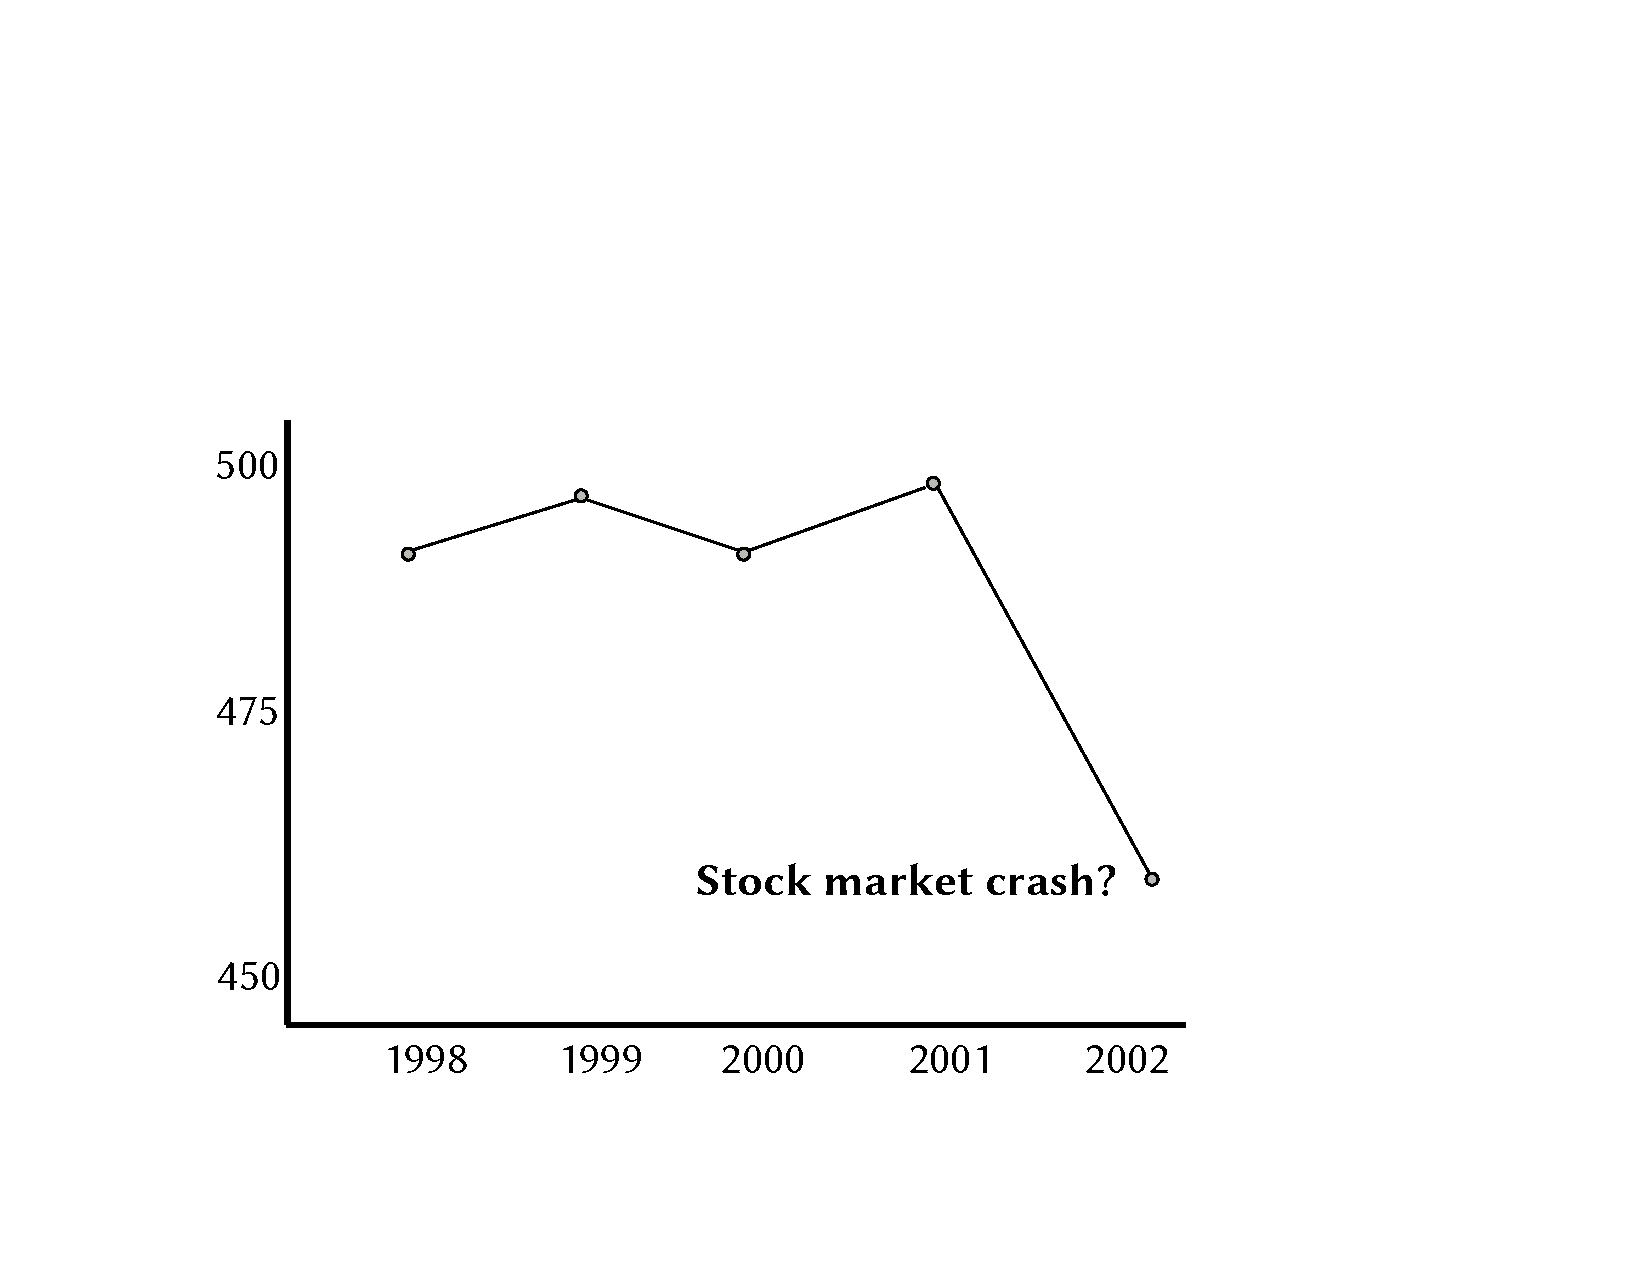
\includegraphics[width=.47\columnwidth]{tufte-integrity-1}} 
\hfill
\subcaptionbox{Using an absolute value range to depict the data accurately.\label{fig:lr-tufte-integrity-2}}{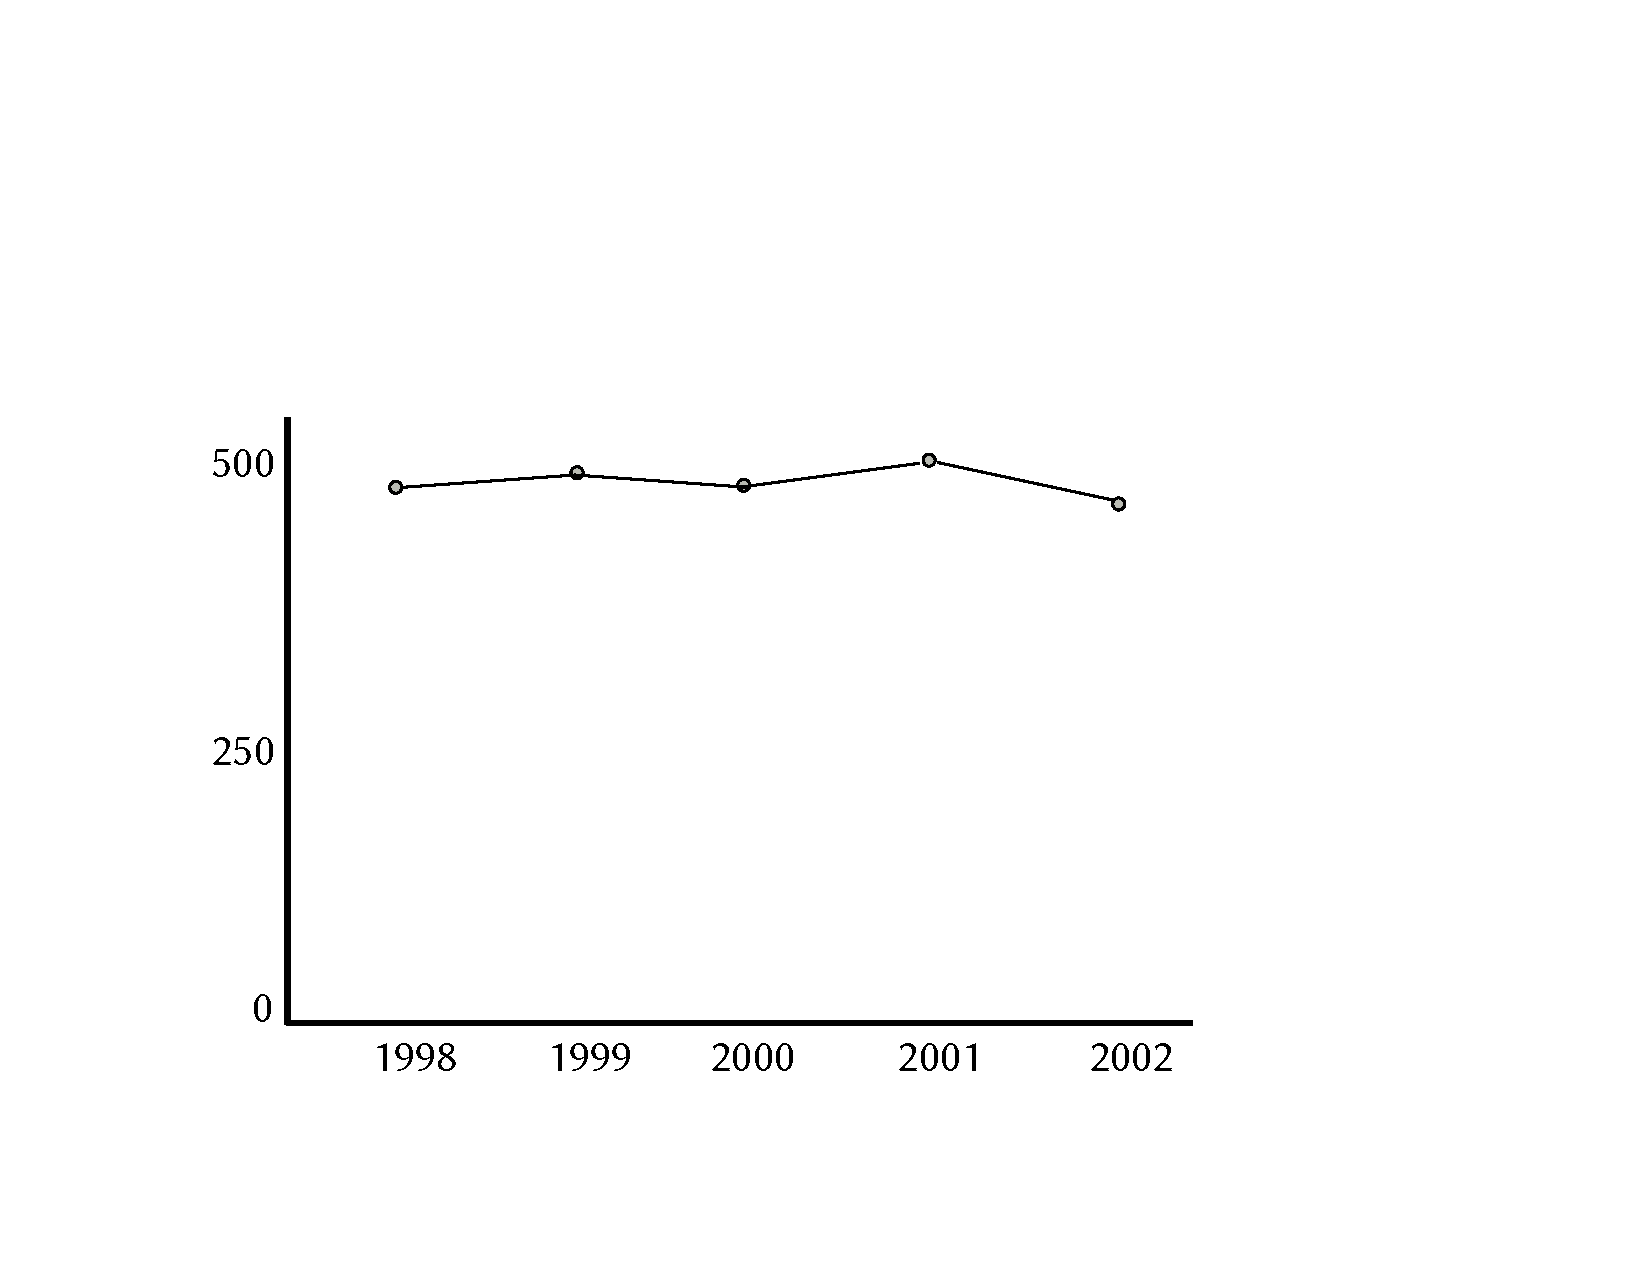
\includegraphics[width=.47\columnwidth]{tufte-integrity-2}} 
\caption{Graphical integrity principle. The chart should tell the truth about the data.}
\label{fig:lr-tufte-integrity}
\end{figure}

\subparagraph{Data-Ink Ratio Maximization}
Data-ink includes the pixels in the graphic that are used for representing the data. Data-ink ratio is defined as the ratio between the data-ink and the total non-background pixels used in the graphic. This principle aims to maximize this ratio by erasing non-data-ink and erasing redundant data-ink.

\begin{figure}[!htb]
\centering
\subcaptionbox{A bar chart with poor data-ink ratio.\label{fig:lr-tufte-ink-1}}{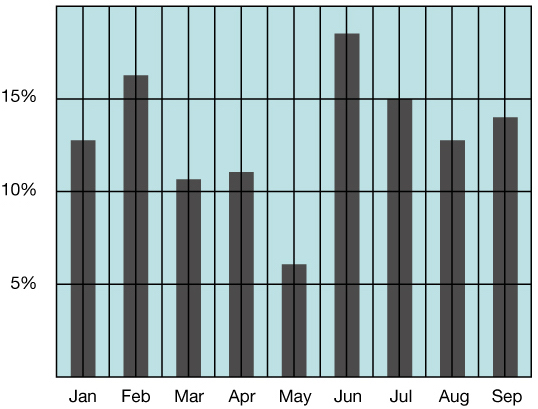
\includegraphics[width=.47\columnwidth]{tufte-ink-1}} 
\hfill
\subcaptionbox{A bar chart with high data-ink ratio by removing background, border and grid lines.\label{fig:lr-tufte-ink-2}}{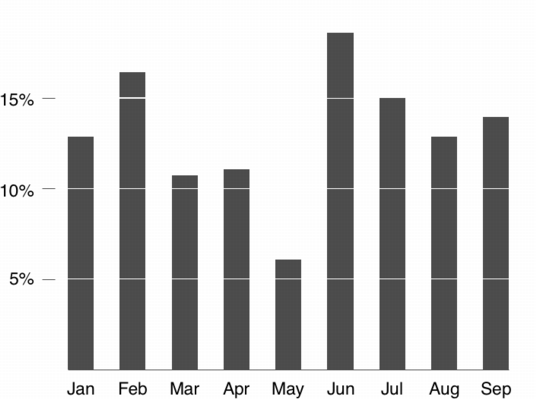
\includegraphics[width=.47\columnwidth]{tufte-ink-2}} 
\caption{Data-ink ratio maximization principle: removing the graphic that does not contribute to the understanding of the data.}
\label{fig:lr-tufte-ink}
\end{figure}
% Source: http://www.infovis-wiki.net/index.php/Data-Ink_Ratio

\subparagraph{Micro/Macro Readings}
This principle suggests that a graphic can contain both enormous details and an overall pattern. This allows the viewer to glance from a distance to observe the big picture, and later drill-down closely to examine its individual pieces. Classic stem-and-leaf plot is a great example to illustrate this principle (\autoref{fig:lr-tufte-micro}). The plot shows all individual data items at meaningful level of detail, and provides an understanding of the data distribution. The micro/macro principle is extensively applied in interactive visualization, where zooming are panning are made possible, such as Google Maps. Data items at different scales can be represented with different levels of detail to provide appropriate information based on the allowed display area.

\begin{figure}[!htb]
	\centering
	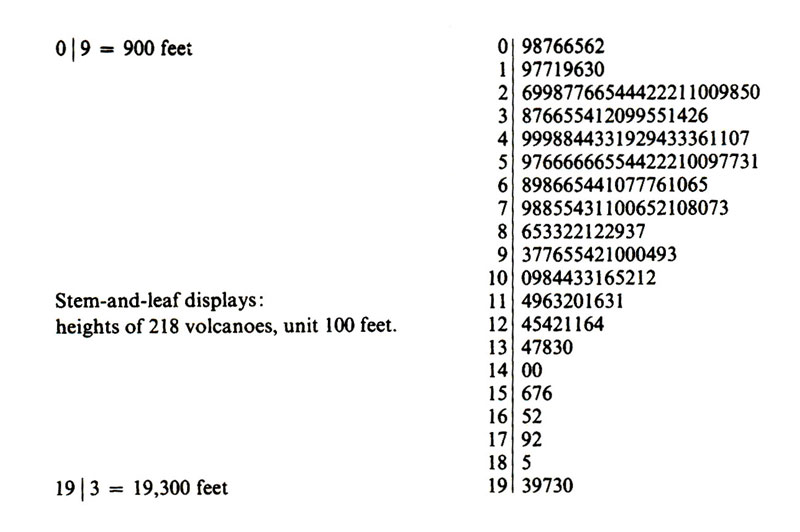
\includegraphics[width=.9\linewidth]{tufte-micro}
	\caption{Micro/macro principle. A stem-and-leaf plot shows both the data distribution and individual items. \is{Tufte1983}}
	\label{fig:lr-tufte-micro}
\end{figure}


%In a broader context, GUI design principles:  Schneiderman~\cite{Shneiderman2016} (eight golden rules), Norman (six design principles) ~\cite{Norman2002} and	Nielsen (ten usability heuristics)~\cite{Nielsen1994} -- create a table with rows showing similar principles
%http://www.csun.edu/science/courses/671/bibliography/preece.html
%https://faculty.washington.edu/jtenenbg/courses/360/f04/sessions/schneidermanGoldenRules.html
%https://www.interaction-design.org/literature/article/shneiderman-s-eight-golden-rules-will-help-you-design-better-interfaces

\subsubsection{Interaction Techniques}
Interaction typically refers to the set of controls provided to the user to manipulate an interface~\cite{Pike2009a}. A static visualization may only show one aspect of a dataset. When the dataset is large enough, showing all the data at once may also make the visualization become cluttered. Interaction plays an important role in solving these problems. It can help explore large datasets at multiple levels of detail, identify patterns through examination of different visual representations and understand the connections between them.

Examples of interaction include standard techniques used in graphical user interface such as mouse clicking and scrolling, and more visualization specific techniques such as \emph{linking and brushing}~\cite{Kosara2003}, and \emph{focus+context}~\cite{Cockburn2008}. Multiple views in a visualization are often linked together to exploit their strengths. The user can select points of interest using the brushing technique, typically done directly on the visual data representation such as dragging a rectangular area. The points are brushed in one view will be highlighted in other views, allowing the user to explore them with different perspectives and representations (\autoref{fig:lr-linking}). Focus+Context is a technique that brings both the overview (context) and the detailed information (focus) together in one view. A fisheye view~\cite{Furnas1986,Furnas2006} is one example of this technique: the focal region is magnified and displayed within its surrounding context (\autoref{fig:lr-fisheye}).

\begin{figure}[!htb]
\centering
\subcaptionbox{Linking and brushing. Data points brushed in one view are linked and highlighted in other views.\label{fig:lr-linking}}{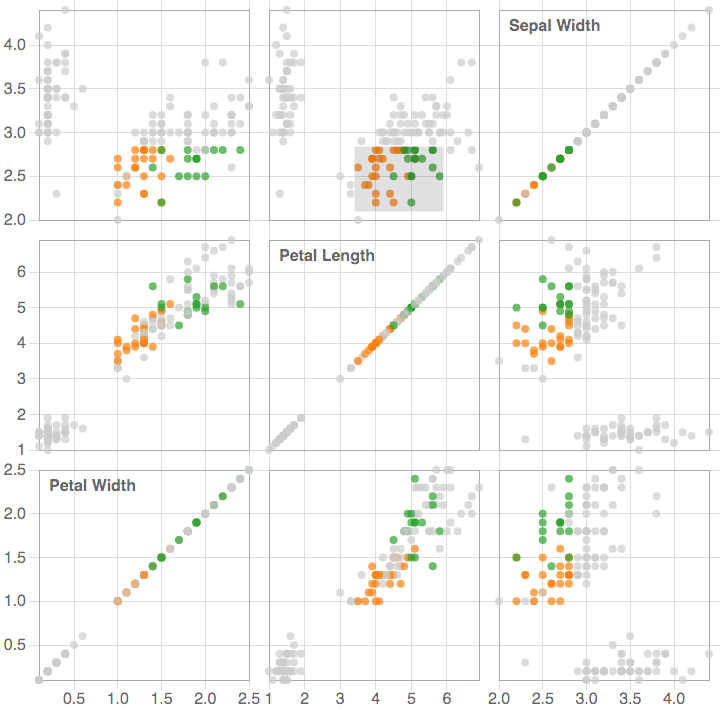
\includegraphics[height=.43\columnwidth]{linking}} 
\hfill
\subcaptionbox{Fisheye view for focus+context. Both the overview and the detailed information are displayed in one view.\label{fig:lr-fisheye}}{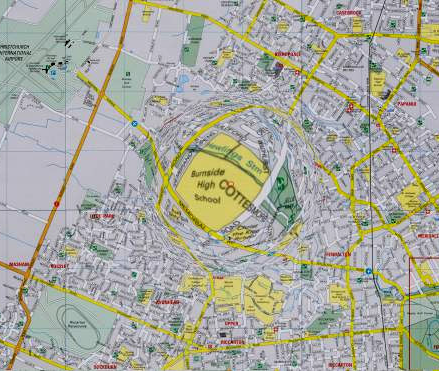
\includegraphics[height=.43\columnwidth]{fisheye}} 
\caption{Examples of interaction techniques.}
\label{fig:lr-interaction}
\end{figure}

Many other interaction techniques can be found in the taxonomies by Dix and Ellis~\cite{Dix1998}, by Keim~\cite{Keim2002}, and by Wilkinson~\cite{Wilkinson2005}. Very often, a user performs an interaction to achieve some goal, thus interaction techniques can also be classified based on their intents. Actually, different interaction techniques in different visualizations may serve the same purpose. For example, both drilling-down a treemap~\cite{Shneiderman1992} and semantic zooming~\cite{Perlin1993} aim to get more details. Taxonomies of high-level interaction can be found in the work by Yi~et~al.~\cite{Yi2007}, by Heer and Shneiderman~\cite{Heer2012}, and by Brehmer and Munzner~\cite{Brehmer2013}. These classifications could help visualization designers select suitable interaction techniques to serve for the capabilities they want to offer to the users.

%Several methods can improve existing different interaction techniques. 
Traditional graphical user interface widgets are often used to control different settings of a visualization, such as buttons and sliders. The disadvantage is that visual feedback does not appear where the interaction happens, but in some parts of the visualization. It also takes time for the user to search for the appropriate setting controllers. Direct manipulation~\cite{Shneiderman1982} is an approach to address these problems. It enables the user to directly interact with the visual representation and receive immediate feedback. One example is using mouse scrolling to adjust zoom level while exploring a map instead of clicking on a button in the toolbar. Another example is parallel coordinates plot with axes can be reordered by direct dragging and values can be filtered by direct brushing on the axes (\autoref{fig:lr-pcp}). Surrogate objects can be used when the data objects are small or distant~\cite{Kwon2011}. An example is the use of interactive legends as filtering means~\cite{Riche2010b}

\begin{figure}[!htb]
	\centering
	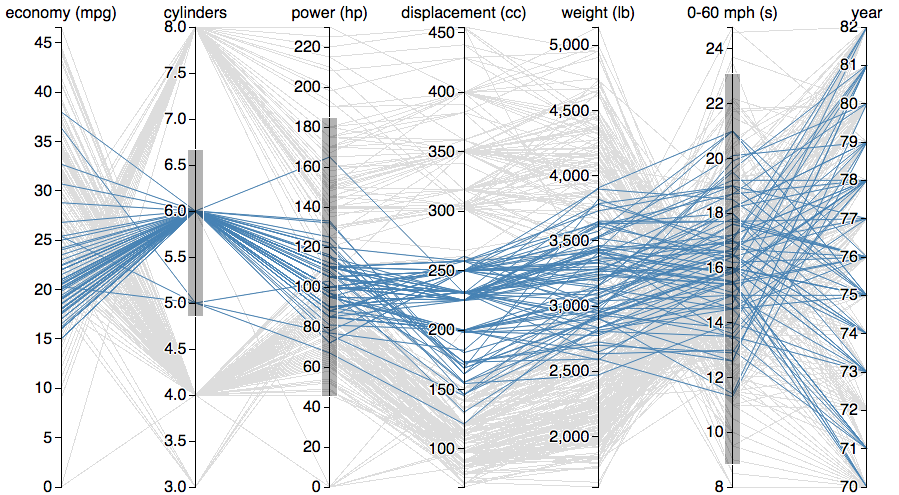
\includegraphics[width=\linewidth]{pcp}
	\caption{Direct manipulation in a parallel coordinates plot with reorder-able and brush-able axes.}
	\label{fig:lr-pcp}
\end{figure}

Another concept that can be applied to improve existing interaction techniques is \emph{fluid interaction}~\cite{Elmqvist2011}. Besides using direct manipulation as discussed previously, the interaction should produce smooth animated transitions between the state before and the state after an interaction, helping users maintain their mental maps; and provide immediate visual feedback, allowing users to know what is happening and/or what will happen next.

Typically, interaction techniques are combined to explore the data or present a known story. A classic visual information-seeking mantra by Shneiderman~\cite{Shneiderman1996} summarizes many design guidelines and interaction techniques for designing information visualizations: \emph{Overview first, zoom and filter, then details-on-demand}. With large datasets, it it challenging to create an overview and provides cues for further exploration. A more suitable approach in this case is \emph{Search, show context, expand on demand}~\cite{VanHam2009}.

\subsection{Automated Analysis Methods}
Data mining is the computational process of extracting patterns in large datasets~\cite{Tan2006}. Data mining tasks can be broadly divided into two major categories:

\begin{itemize}
		\item \emph{Descriptive tasks}. The objective is to derive patterns (correlations, trends, clusters, trajectories and anomalies) that summarizes the underlying relationships in data. Examples include cluster and association analyses. \emph{Clustering} aims to split data items to groups so that items within a group are more similar to each other than those in other groups. For example, clustering can be used to help marketers discover distinct groups of their customers before applying appropriate marketing strategies to those groups. \emph{Association} analysis discovers the connections among a set of data items. For example, it can be used to identify products that customers often purchase together such as bread and milk.
		
		\item \emph{Predictive tasks}. The objective is to predict the value of an unknown (target) attribute based on the values of other (explanatory) attributes. Examples include classification and regression. \emph{Classification} predicts discrete target variables whereas, \emph{regression} focuses on continuous ones. For example, predicting whether a customer buys a marketing product is a classification task because the target variable is binary. However, estimating a future house price is a regression task because price is a continuous-valued variable.
\end{itemize}

Next, we will discuss the clustering and classification tasks in more detail and how they are applied together with visualizations to help users gain deeper insight into the data. We also present some commonly used text mining techniques for exploring large sets of documents, which is essential in visual analytics~\cite{Thomas2005}.

\subsubsection{Clustering}

\paragraph{Overview}
Cluster analysis finds similarities between data points based on the characteristics of data attributes and groups similar data points into clusters. Clustering is regarded as \emph{unsupervised learning}~\cite{Han2011} because it can reveal hidden structure of a dataset that does not have \emph{labels} (or groups) defined. The most common clustering algorithm is \emph{k-means}~\cite{Lloyd1982}. Given a set of data points $(x_1, x_2, \dots, x_n)$, k-means clustering aims to partition them into $k$ clusters $(S_1, S_2, \dots, S_n)$, such that the within-cluster sum of squared distances is minimized: 
\[
\sum_{i=1}^k\sum_{x\in S_i} \lVert x-\mu_i \rVert^2
\]
where $\mu_i$ is the center of points (i.e., centroids) in $S_i$. 

The algorithms works as follows. Initially, partition data points into $k$ non-empty random subsets. Then, compute the centroids of the current clusters, and assign each data point to the cluster with the nearest centroid. Repeatedly recompute the centroids and reassign the cluster of each data point until no assignment can be done. This k-means clustering algorithm is efficient but often terminates at a local optimal. More detailed analysis of k-means and other clustering algorithms are out of the scope of this thesis and can be found in data mining textbooks~\cite{Tan2006,Han2011}.

\paragraph{Application Examples}
Human motion tracking data has been applied in various research fields such as medicine, sports and animation~\cite{Bernard2013}. The data consists of temporal sequences of human poses represented by a set of 3D joint positions (e.g., head, hands, elbows and knees). However, analyzing a large collection of such temporal and high-dimensional datasets is challenging. To gain an overall understanding of the data, MotionFlow~\cite{Jang2016} applies a k-means clustering method using a simple Euclidean distance of 3D joints as the similarity measurement. A cluster of human poses is represented as a glyph with a stick figure showing the centroid of the cluster and semi-transparent ghosts around the center figure for other similar poses (\autoref{fig:lr-MotionFlow}).

\begin{figure}[!htb]
	\centering
	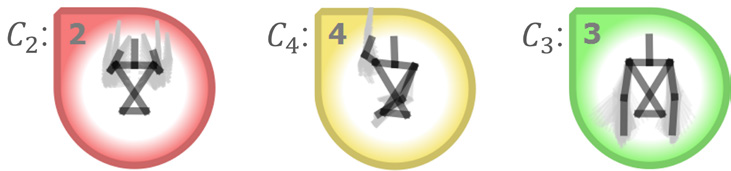
\includegraphics[width=.8\linewidth]{clus-MotionFlow}
	\caption{Visual representation of human pose clusters. \is{Jang2016}}
	\label{fig:lr-MotionFlow}
\end{figure}

MotionFlow uses a force-directed graph of clusters to illustrate their relationship with node distance mapping to the similarity of pose clusters and edges indicating the directed transition between two clusters. Edges are color coded to represent the transition frequency. A user is allowed to interactively change the number of clusters, enabling exploration of the dataset. However, the re-clustering process may change all existing clusters and make it difficult for the user to keep track. To address this issue, MotionFlow allows the user to select the clusters to be locked or unchanged during the re-clustering process. He or she is also able to interactively merge or split clusters according to his or her own assessment.

To achieve the same objective of gaining an overall understanding of human motion tracking data, MotionExplorer~\cite{Bernard2013} applies a different cluster analysis method -- hierarchical clustering~\cite{Han2011} -- which seeks to build a hierarchy of clusters. MotionExplorer takes a divisive approach considering all data items starting within the same cluster and splitting them until a termination condition is met. One of the important decisions in this clustering technique is to determine which cluster to split next. The user is allowed to choose among several splitting strategies such as \emph{maximum standard deviation} to split the most varied cluster first and \emph{highest number of elements} to split the largest cluster first. The hierarchy is visualized as a dendrogram as in \autoref{fig:lr-MotionExplorer}. Clusters are obtained by cutting the dendrogram at the desired vertical level: each connected branch forms a cluster. The vertical axis of the dendrogram can encode different variables depending on the splitting strategy. In \autoref{fig:lr-MotionExplorer}, it shows the standard deviation of each cluster and the user is allowed to slide the cutting value to adjust the resulting clusters.

\begin{figure}[!htb]
	\centering
	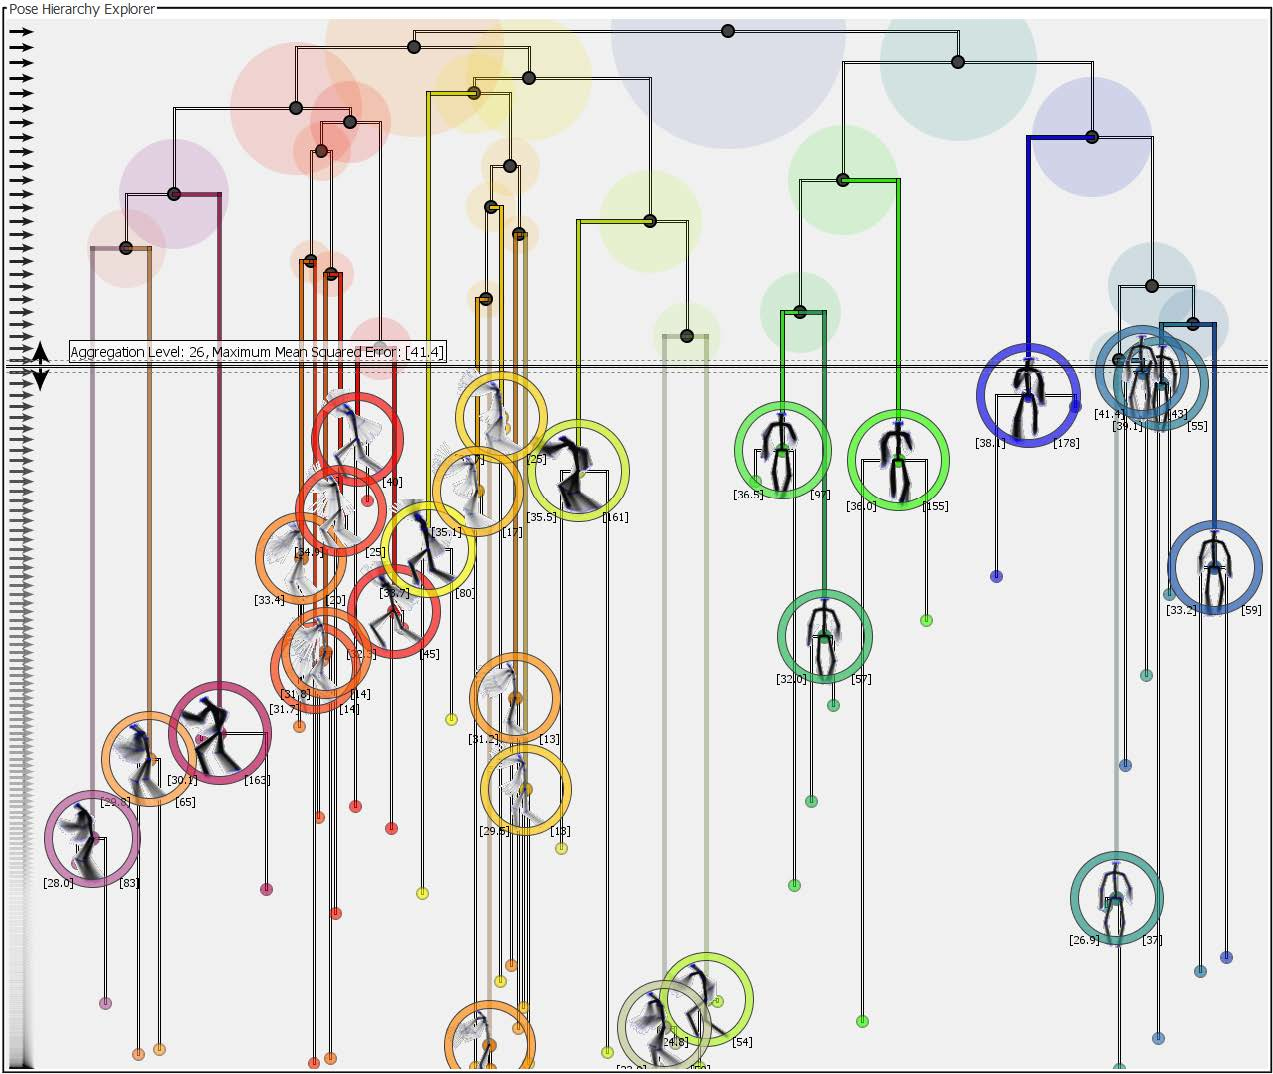
\includegraphics[width=\linewidth]{clus-MotionExplorer}
	\caption{A divisive hierarchical clustering of human poses visualized as a dendrogram. \is{Bernard2013}}
	\label{fig:lr-MotionExplorer}
\end{figure}

A different approach in hierarchical clustering is bottom-up or agglomerative clustering. The process starts with singleton clusters before merging the most similar clusters together until a termination condition is met. NewsLab~\cite{Ghoniem2007} applies such an approach in analysis of large scale broadcast news video collections. It builds a hierarchy of clusters over all keywords extracted from available video captions based on their co-occurrences in the news stories. Therefore, strongly correlated keywords are grouped into the same clusters whereas loosely related keywords are separate in different clusters. Each cluster is visualized as a stream showing the evolution of the keywords within the cluster over time with closely related clusters placed close to each other to allow navigation to different depths of the cluster hierarchy (\autoref{fig:lr-NewsLab}).

\begin{figure}[!htb]
	\centering
	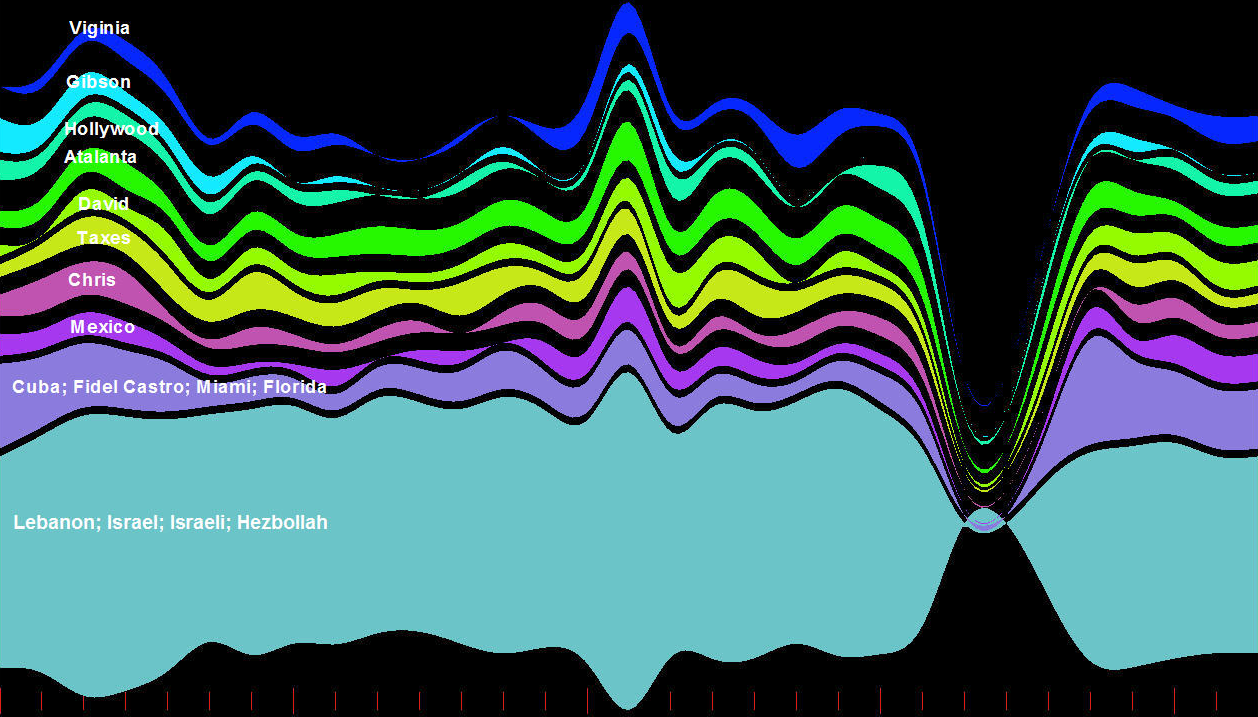
\includegraphics[width=\linewidth]{clus-NewsLab}
	\caption{An agglomerative hierarchical clustering of video captions visualized as streams. \is{Ghoniem2007}}
	\label{fig:lr-NewsLab}
\end{figure}

Understanding people movement patterns in both space and time plays an important role in urban planing. Analyzing and presenting large and complex datasets that contain a number of people in different places and their movement between those places over time are challenging. Mobility Graphs~\cite{Landesberger2016} applies cluster analysis to simplify the data in both spatial and temporal dimensions to gain an overall understanding of the datasets. First, it aggregates places using a density-based clustering technique that considers both the density of places and their flow magnitudes so that close and highly connected can be grouped together. Second, temporal aggregation groups the time steps by the similarity of those simplified places using a k-means clustering technique. \autoref{fig:lr-MobilityGraphs} shows 7 temporal clusters of simplified places. The clusters are color coded with a calendar view to reveal temporal patterns over a week. In each cluster, a node shows an aggregated place with size corresponding to the total number of people in all individual places and arrow widths representing the number of people moving between two aggregated places.

\begin{figure}[!htb]
	\centering
	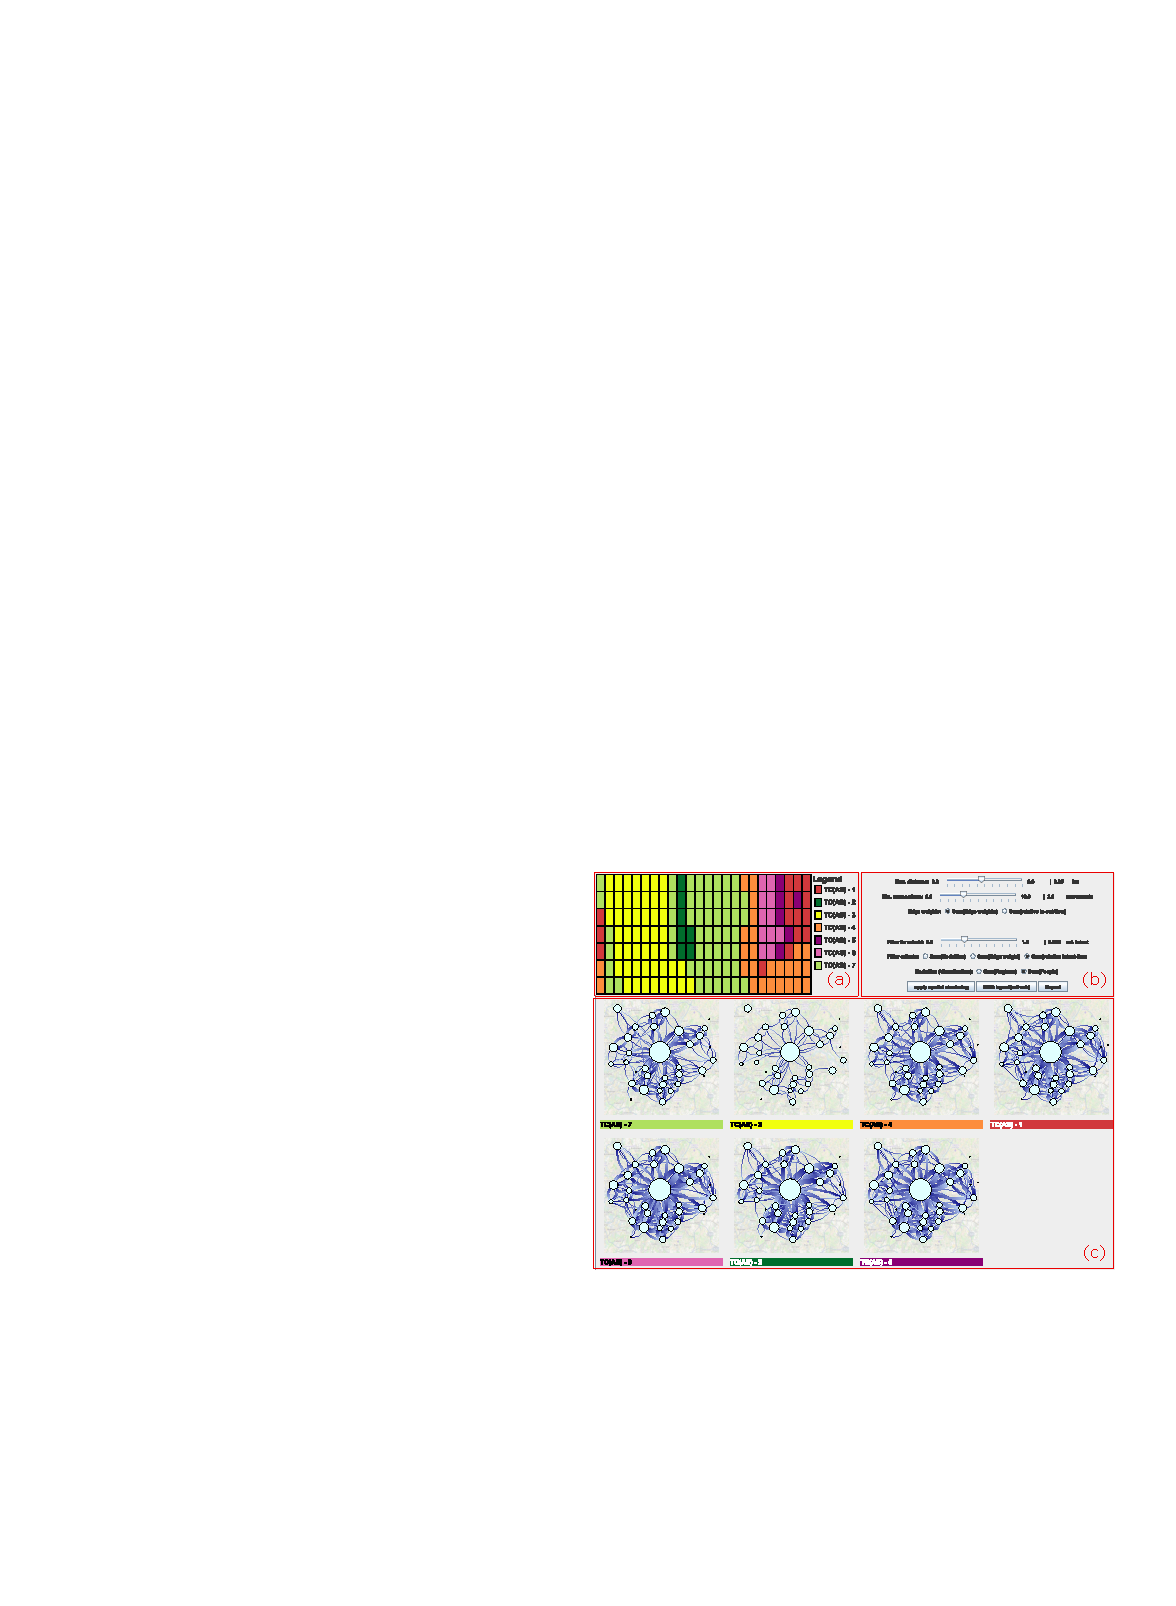
\includegraphics[width=\linewidth]{clus-MobilityGraphs}
	\caption{Temporal clusters of simplified places. \is{Landesberger2016}}
	\label{fig:lr-MobilityGraphs}
\end{figure}

\subsubsection{Classification}
\paragraph{Overview}
Classification predicts the value of a categorical (discrete or nominal) attribute based on the values of other attributes. It builds a model (or \emph{classifier}) based on a labeled training dataset (i.e., \emph{supervised learning}) and applies it in labeling new data~\cite{Han2011}. The model needs to not only identify the labels in the training dataset well but also be general enough to predict the labels of new data correctly. One common and intuitive classification algorithm is decision tree induction~\cite{Quinlan1986}. Each non-leaf node represents a ``test'' on an attribute, which splits the node to multiple branches, each for an outcome of the test. Each leaf node is associated with a class label and is the result of a sequence of tests starting from the root node.

The importance of building a decision tree is choosing which attribute to split at each node. Intuitively, we should choose attributes that can divide nodes into ``pure'' child nodes so that all data items in a child node belong to a single class and no further splits is needed. For example, in a binary classification, consider a training dataset with 10 records, 5 labeled ``true'' and 5 labeled ``false''. Attribute $A1$ splits the set to two subsets: (5 ``true'', 0 ``false'') and (0 ``true'', 5 ``false''). Attribute $A2$ splits the set to (3 ``true'', 2 ``false'') and (2 ``true'', 3 ``false''). The subsets split by $A1$ is ``purer'' than the one by $A2$ because they do not contain a mix of ``true'' and ``false''. To achieve this purity, several attribute measurements have been proposed such as \emph{information gain} and \emph{gini index}~\cite{Tan2006}. More detailed analysis of these measurements and other classification algorithms are out of the scope of this thesis and can be found in data mining textbooks~\cite{Tan2006,Han2011}.

\paragraph{Application Examples}
Exploring a large image collection, such as the set of images available on the Internet, is challenging. Besides the low-level visual features, the semantic contents of images are also effective in searching for relevant ones. Image classification techniques can be used to extract such semantic contents. For example, Fan~et~al.~\cite{Fan2004} detect salient objects in images and associate them with predefined semantic contents according to their perceptual properties. Similar contents are then grouped into a higher level semantic concept; for instance, ``sand field'', ``sea water'' and ``boat'' salient objects construct the concept of ``sea world''. Visualization can help make the output of classification algorithms more interpretable and interactive. To provide an overview of an image collection, Yang~et~al.~\cite{Yang2006} shows the extracted semantic contents, with each as a glyph, in a 2D display so that related contents are located close together using a multidimensional dimension scaling method~\cite{Borg2005}. Similarly, images are also displayed based on their similarity as in \autoref{fig:lr-SIBa}. Zooming and panning are provided to make the visualization more scalable. When an image is selected, the visualization can be switched to a \emph{rainfall} mode, in which the selected image is shown at the bottom and related images are stacked above it based on their similarity with the selected one (\autoref{fig:lr-SIBb}). Users are allowed to reassign the contents computed for each image; however, the model does not take into account the changes to improve its accuracy when classifying new images.

\begin{figure}[!htb]
\centering
\subcaptionbox{Multidimensional dimension scaling view of images.\label{fig:lr-SIBa}}{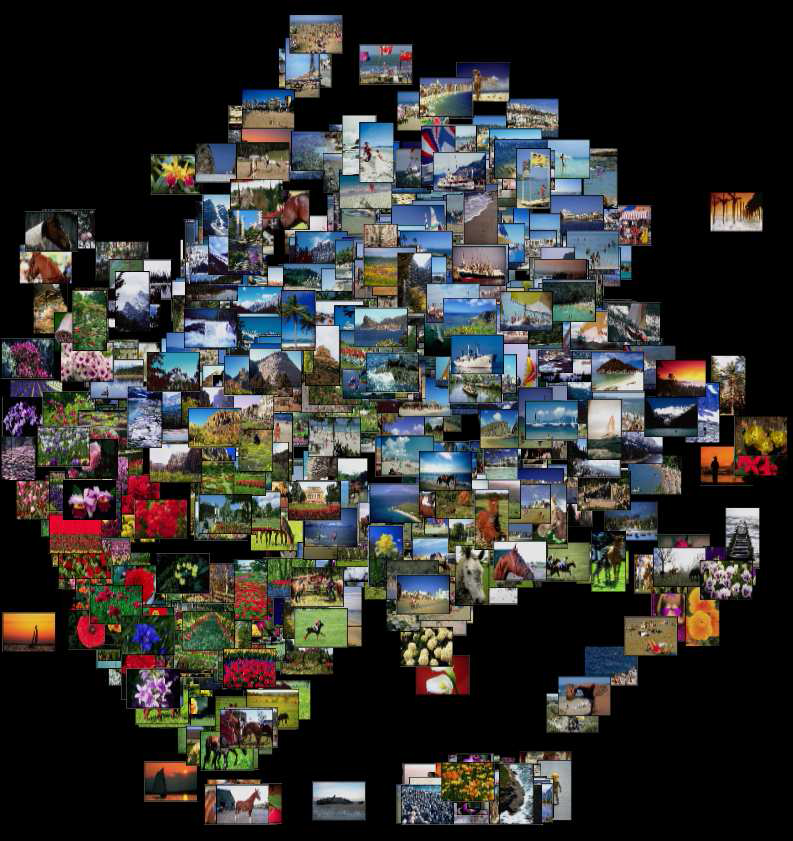
\includegraphics[height=.5\columnwidth]{clas-SIBa}} 
\hfill
\subcaptionbox{Rainfall view of a selected image with highly related images at the bottom.\label{fig:lr-SIBb}}{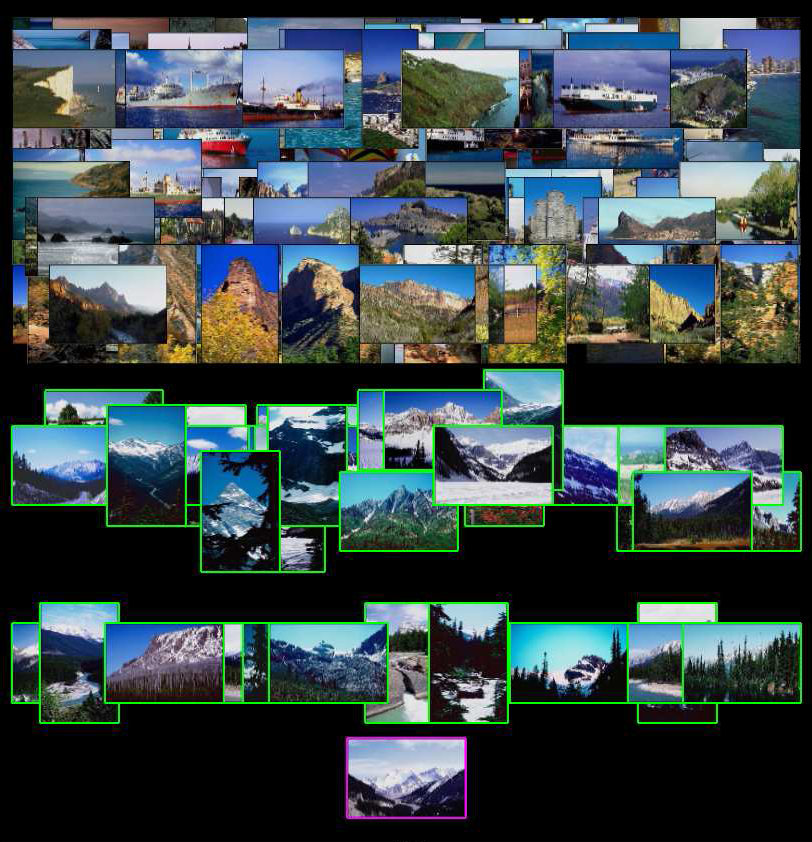
\includegraphics[height=.5\columnwidth]{clas-SIBb}} 
\label{fig:lr-SIB}
\caption{Semantic image browser. \is{Yang2006}}
\end{figure}

In a binary classification, the classifier output is either \emph{positive} or \emph{negative}. Two types of error can happen include \emph{false positive} (classified as positive but the actual class is negative) and \emph{false negative} (classified as negative but the actual class is positive). Depending on a domain, the costs of these error types might be considerably different. For example, wrong prediction of a healthy patient with a cancer has a much lower impact than missing a patient with a real cancer. Migut and Worring~\cite{Migut2010} allow users to adjust the trade-off between these two error types through the visualization of the classification model. Typically, a receiver operating characteristic curve~\cite{Fawcett2006} is used to illustrate the performance of a binary classifier as its discrimination threshold is varied. The curve is composed from a set of true positive rate and false positive rate pairs at various threshold values. Migut and Worring~\cite{Migut2010} replace the true positive rate with the false negative rate (\autoref{fig:lr-Migut1}) because their focus is comparing trade-off between the two error rates. Numerical data is visualized in a scatter plot with the decision boundary separating a 2D plane into two regions, each for a class (\autoref{fig:lr-Migut2}). For each data point, color shows the original class and size indicates the accuracy of the classified class. The current classification setting is shown as a red point on the performance curve, and the user is allowed to move that point along the curve to change the false positive and false negative rates. The classification reruns with the new threshold and rates and updates on the data scatter plot.

\begin{figure}[!htb]
\centering
\subcaptionbox{Performance curve of the classification model with horizontal axis showing the false positive rate and vertical axis showing the false negative rate. rates.\label{fig:lr-Migut1}}[\columnwidth]{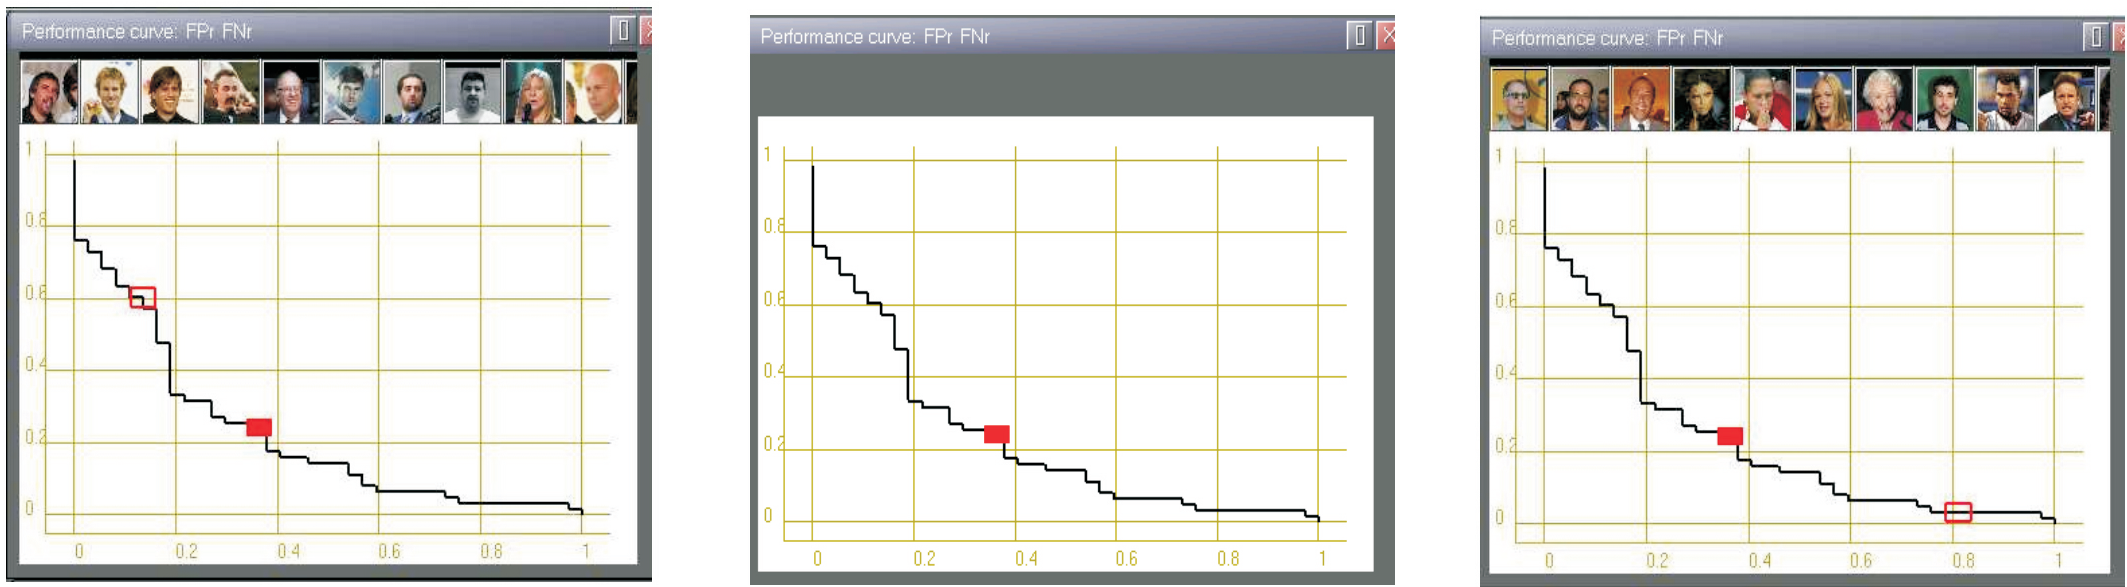
\includegraphics[width=\columnwidth]{clas-Migut1}} 
\\
\subcaptionbox{Data with color indicating original class and size showing classification accuracy.\label{fig:lr-Migut2}}[\columnwidth]{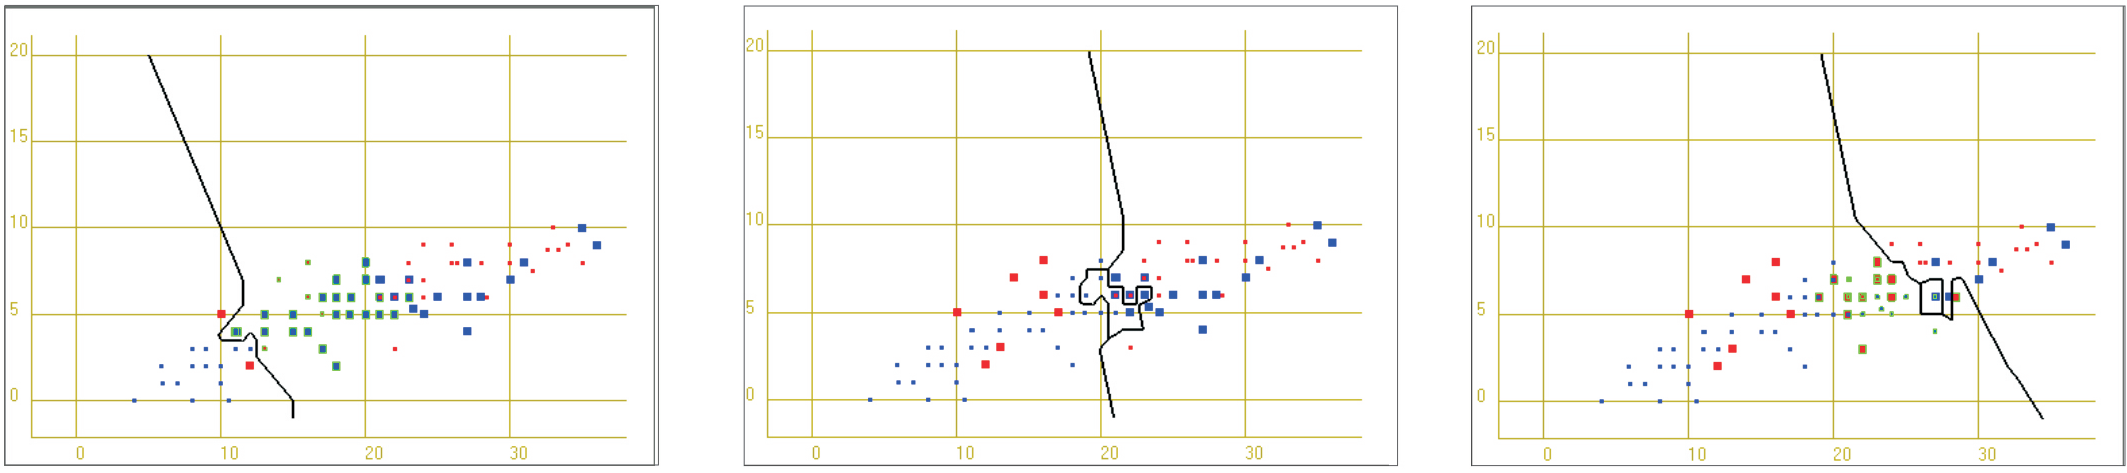
\includegraphics[width=\columnwidth]{clas-Migut2}}
\caption{Visualization and interaction of a classification model. Figure in the middle shows the initial state of the system, with initial operating point on the performance curve and corresponding data scatter plot. Figure on the left shows the state of the system when an expert manipulates the operating point to include more false negatives and on the right to include more false positives. \is{Migut2010}}
\end{figure}

Classification requires training data; however, it can be time-consuming and laborious to produce such a dataset. ScatterBlogs2 includes an interactive classifier that speed up the training data labeling and classifier construction before applying it in real-time monitoring messages of interest~\cite{Bosch2013}. First, the user can search for relevant messages using a standard keyword query. The system then highlights non-trivial terms that frequently co-occur with the original keywords. The result set of highly relevant messages can be used as \emph{positive} samples, whereas some arbitrary messages not returned in the result set can be used as \emph{negative} ones. After creating an initial classifier, the user can inspect messages to correct and update the classifier through the message visualization. Messages are shown in a map as a colored glyph with color hue indicating class and brightness showing classification confidence (\autoref{fig:lr-ScatterBlogs2}). Messages can be filtered by confidence, allowing the user to focus on ones with less certainty, which need human expert to verify. To further speed up the classifier creation, ScatterBlogs2 offers self-training, a technique that iteratively uses messages classified with the highest confidence as labeled data. 

\begin{figure}[!htb]
	\centering
	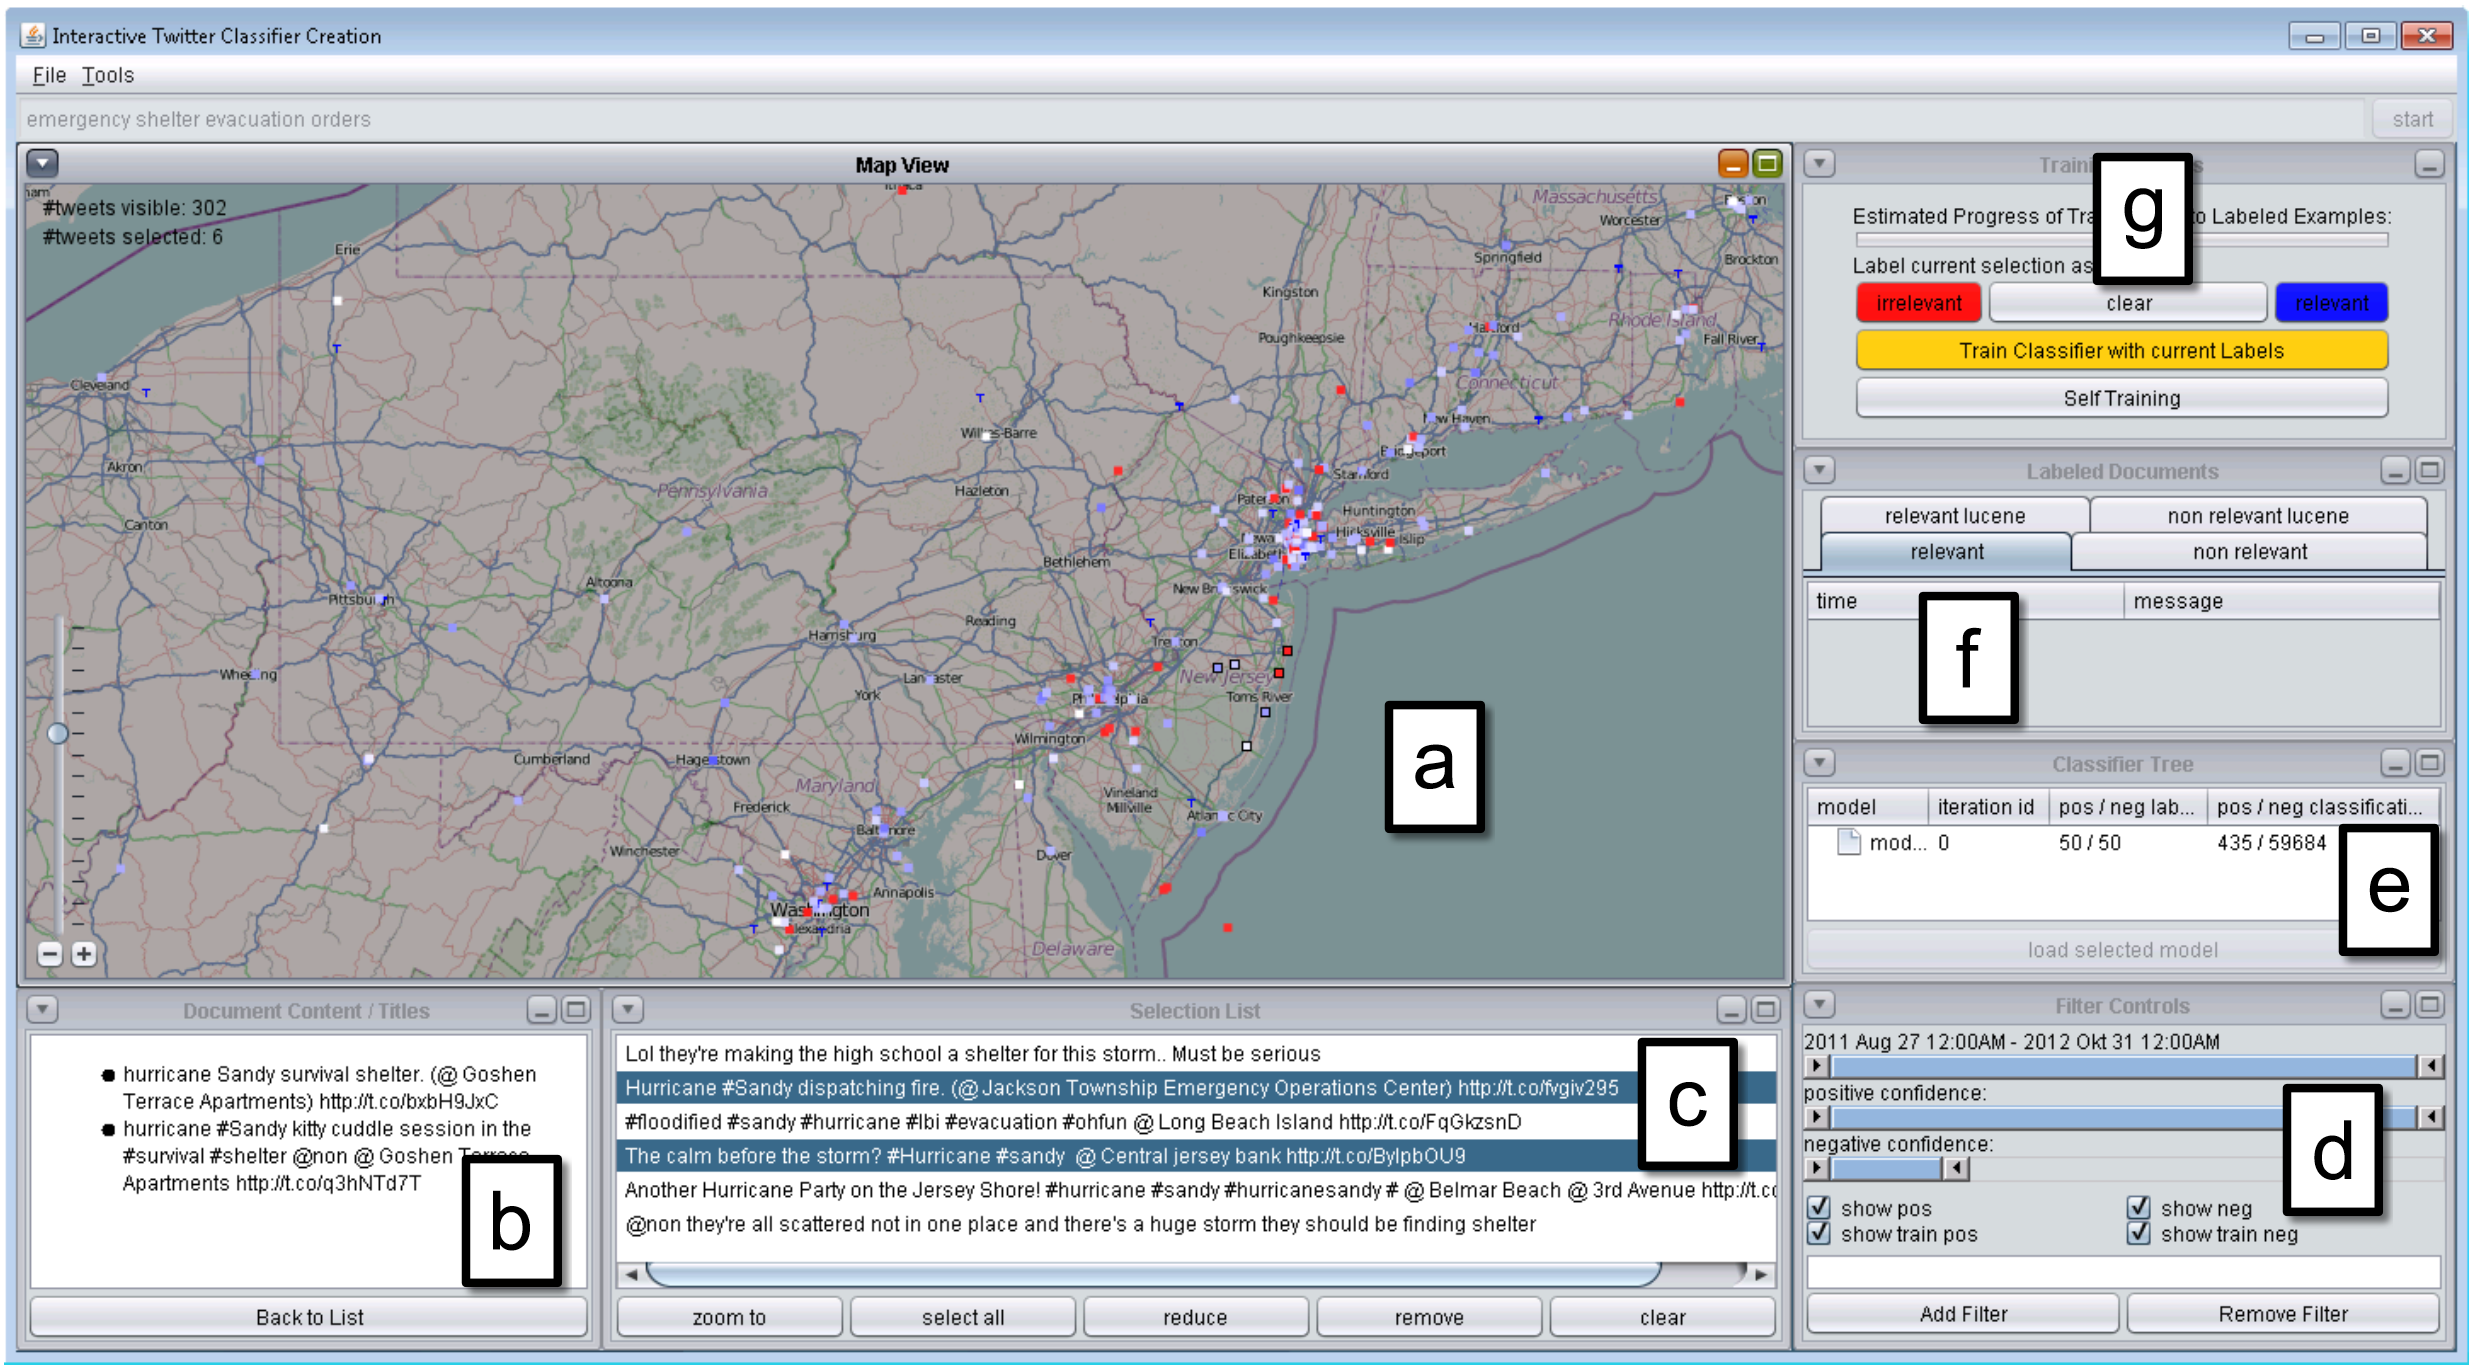
\includegraphics[width=\linewidth]{clas-ScatterBlogs2}
	\caption{The classifier creation environment of ScatterBlogs2. \is{Bosch2013}}
	\label{fig:lr-ScatterBlogs2}
\end{figure}

An essential step in classification of high dimensional datasets is feature selection, which selects a subset of relevant features for use in model construction without much loss of information. This step also simplifies the model and reduces training time. INFUSE~\cite{Krause2014} supports users to explore the predictive power of features in their models. The system allows comparison of features across four feature selection algorithms. Each feature is shown as a circle glyph divided into four equal quadrants, each for an algorithm (\autoref{fig:lr-INFUSE}). A quadrant is further split into 10 slices, each for a cross-validation fold (or random subset of data) to ensure the result  robust. The length of a slice indicates the rank of that feature using a given algorithm. Therefore a glyph can show how its feature performs in different algorithms. To have an overview of all features, INFUSE shows multiple glyphs in either a sequential layout or a scatter plot, where different options can be used for axes such as average rank of a feature or a more sophisticated importance measurement. It also allows users to explore four classification algorithms by showing the score of all 16 combination of feature selection and classification algorithms. More importantly, users are allowed to build their own model by selecting features besides the ones produced by the four given algorithms. The custom feature set is then included in the classification score comparison.

\begin{figure}[!htb]
	\centering
	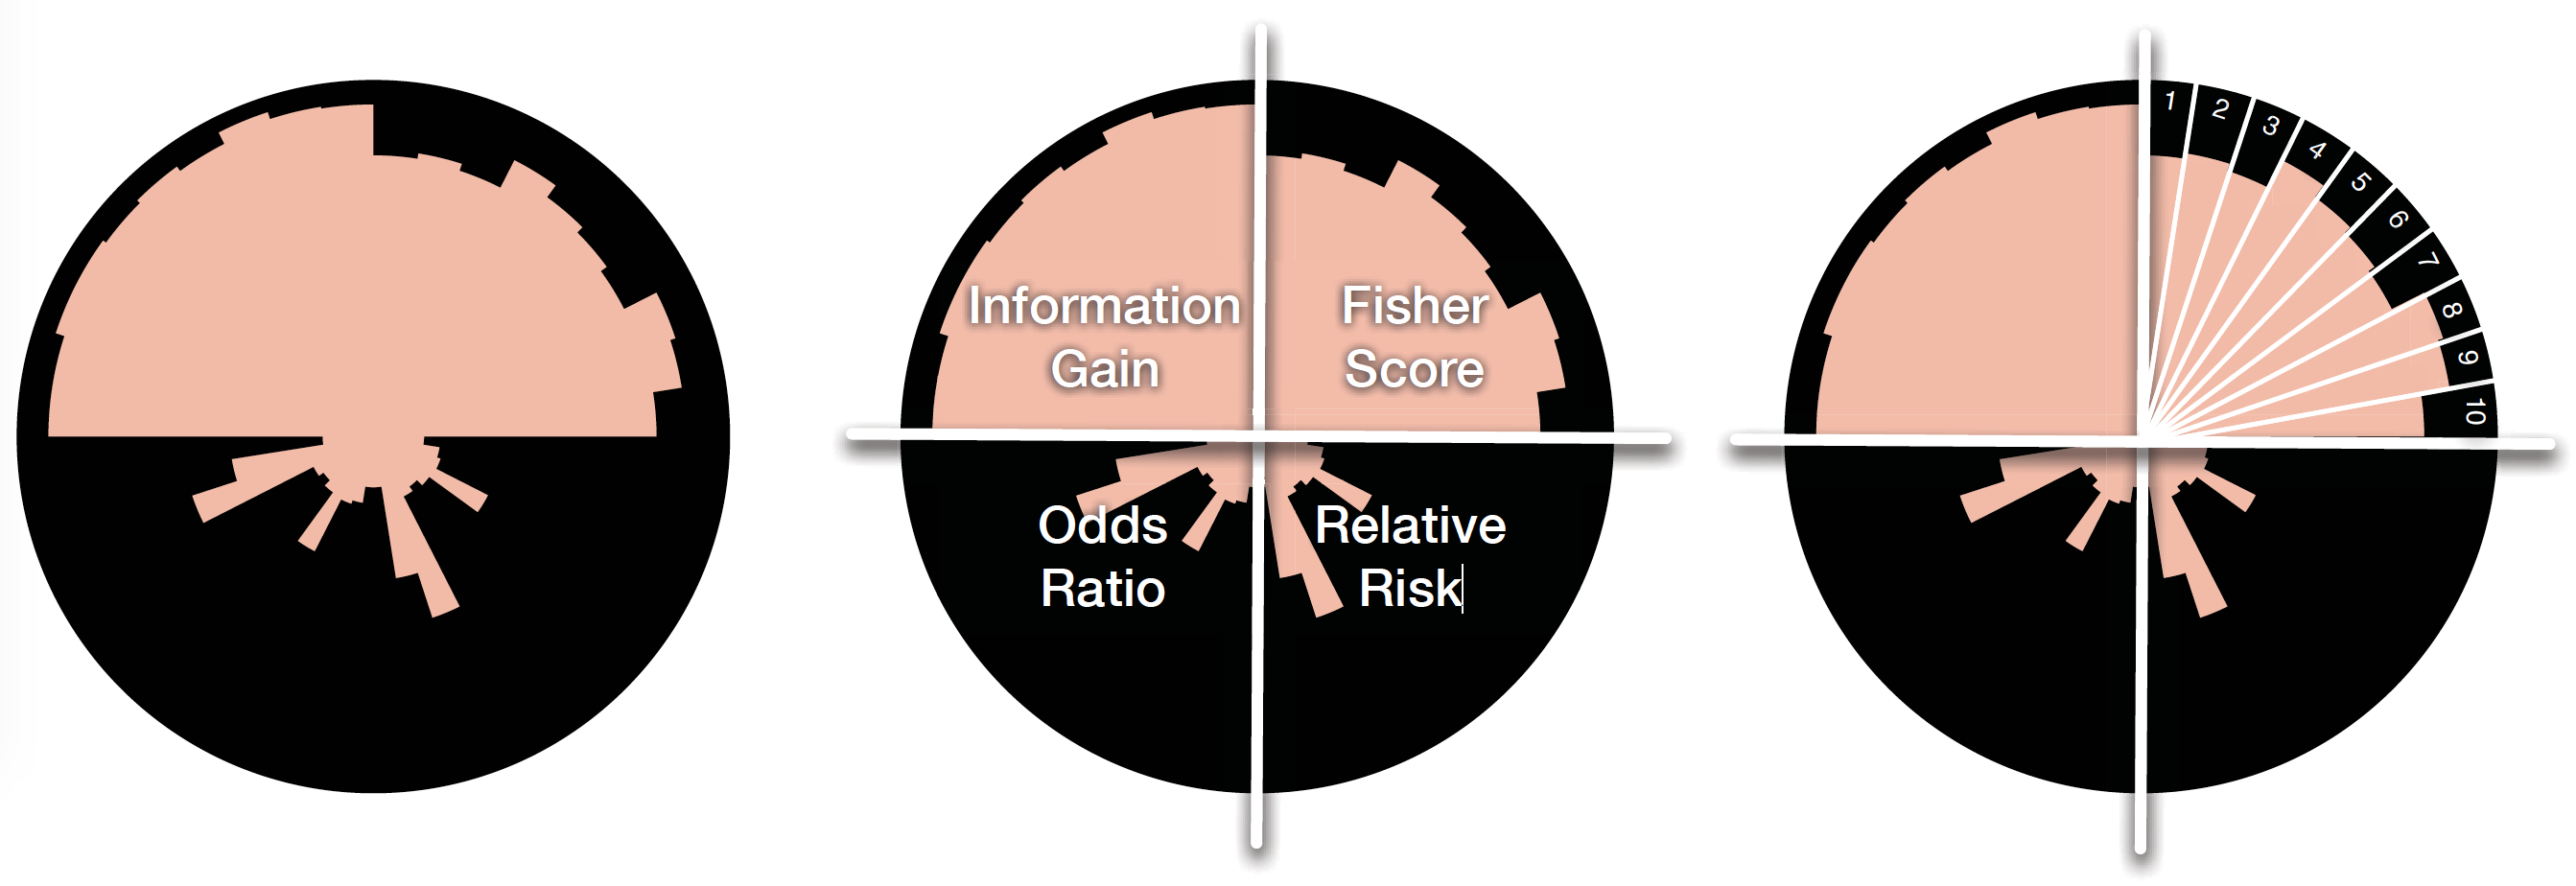
\includegraphics[width=\linewidth]{clas-INFUSE}
	\caption{The feature glyph in INFUSE. \is{Krause2014}}
	\label{fig:lr-INFUSE}
\end{figure}

\subsection{Evaluation Methods}
A visualization, no matter how novel and interesting it is, needs to be evaluated to check whether it meets the design goals and supports the target users to complete the intended tasks. Evaluation has been a research topic in visualization when the field becomes more matured~\cite{Plaisant2004}. Excellent reviews of visualization evaluation with different perspectives include evaluation techniques~\cite{Carpendale2008}, scenarios~\cite{Lam2012} and design process~\cite{Munroe2009}.

In this section, we review the evaluation techniques based on the visualization design model by Munzner~\cite{Munroe2009}, helping address different concerns separately. The four levels include: explain the tasks and available data in the vocabulary of the problem domain, abstract them into domain-independent operations and data types, design visual encoding and interaction techniques to solve the abstract tasks, and develop algorithms to execute these techniques efficiently. Each level has its own \emph{threats} to validity and methods to address them. Two types of methods are distinguished: \emph{immediate} approaches can be done before inner levels are implemented, whereas \emph{downstream} approaches requires all inner levels are completed. The threats and evaluation methods are summarized in \autoref{fig:lr-nested-model}.

\begin{figure}[!htb]
	\centering
	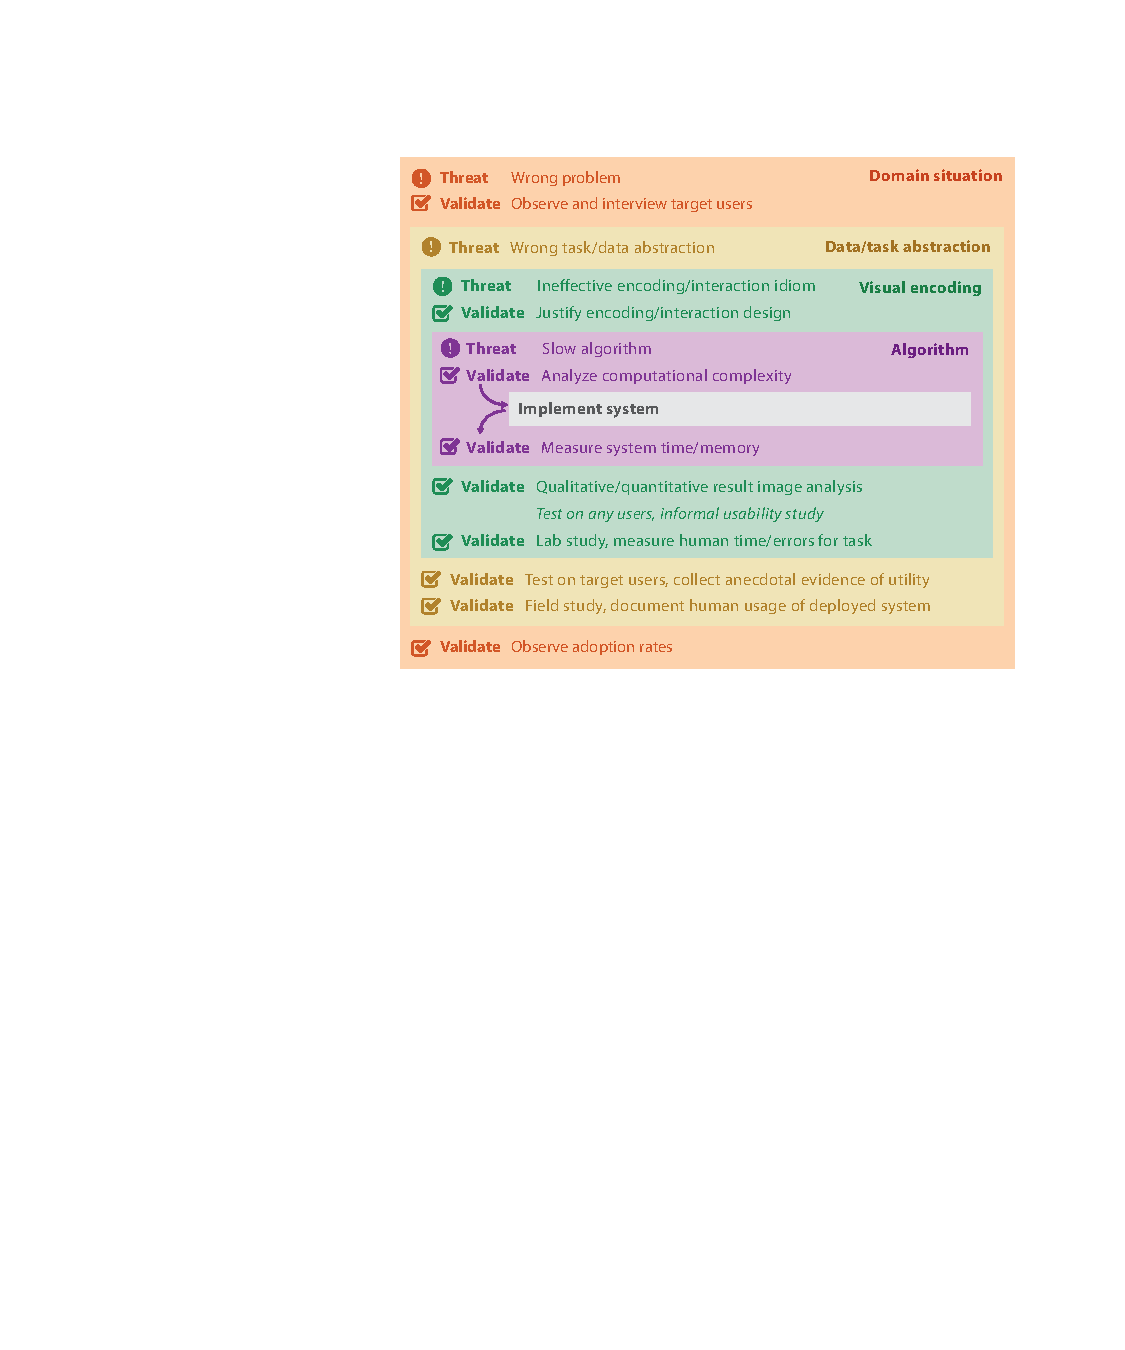
\includegraphics{nested-model}
	\caption{Threats and validation at each of the four nested levels of visualization design. \is{Munzner2014}}
	\label{fig:lr-nested-model}
\end{figure}

\subsubsection{Domain Problem and Data Characterization}
The domain problem of target users is investigated to see if visualization is a potential solution. The primary threat is that the problem is mischaracterized: the users do not really suffer from the identified problem. An immediate form of validation is \emph{field study}~\cite{Carpendale2008}, where the investigator observes how target users act in real-world settings in order to learn and verify the characterization. Another technique is \emph{contextual inquiry}~\cite{Holtzblatt1993}, which allows the investigator to occasionally interview while the user is engaged in the process. One example is the study by Sedlmair~et~al.~\cite{Sedlmair2008} on current working behavior and environments of analysis and diagnosis experts in the automotive industry.

One downstream form of validation is to report the rate the adoption rate of the tool by the target users. High effort is required to make the visualization solution reliable and deployable in the real-world environment. Examples include a field study of Google's Notebook product~\cite{Russell2008} and 6-week field trial of SparTag.us -- a tagging system for foraging web content~\cite{Hong2008}.

\subsubsection{Operation and Data Type Abstraction}
The threat at this level is the identified data and task abstraction do not solve the characterized problem. Only downstream approaches can be used to validate the abstraction. The deployed system needs to be used by target users completing their routine tasks in real-world environment. The goal of this evaluation is to collect anecdotal evidence that the solution is in fact useful. The observation and interview need to focus on understanding how the tool is used, and how it helps or hinders the users in performing their tasks. An example is a longitudinal field study of LiveRAC system that supports analysis of system management time-series data~\cite{McLachlan2008}.

Evaluating the visualizations for supporting sensemaking can be done at this level, as the \emph{evaluating visual data analysis and reasoning} scenario in the taxonomy by Lam~et~al.~\cite{Lam2012}. Due to the nature of sensemaking, evaluation is often carried out as case studies~\cite{Kang2011} with observation and interview, and followed by qualitative data analysis~\cite{Lazar2010}. Attempts also have been made to quantify the insight or knowledge gained during sensemaking~\cite{Wilson2013}.

\subsubsection{Visual Encoding and Interaction Design}
At the design level, the threat is the chosen design is ineffective at communicating the desired abstraction to the user. One immediate form of validation is to justify every design decision based on known design principles such as the ones discussed in \autoref{sub:lr-design}, or more comprehensive predefined guidelines as in heuristic evaluation~\cite{Zuk2006}. Asking experts to review the design prototype also provides valuable feedback~\cite{Tory2005}.

A common downstream approach is to conduct a controlled experiment comparing the design with other state-of-the-art alternatives~\cite{Xu2012}. A number of participants, depending on the  expected size of the experiment, carry out a number of tasks representing real-world cases. Typically, task completion time and accuracy are measured and analyzed using hypothesis testing methods~\cite{Field2003}. Post-task interviews are often combined to establish deeper understanding about how the visualization is used. If the experiment can be completed online, crowd-sourcing approach using Amazon's Mechanical Turk service can help largely increase the size of participants~\cite{Heer2010a}. Another downstream approach is the measurement of common aesthetic metrics such as the number of edge crossings and edge bends that have been used in graph visualization~\cite{Sugiyama1981}.

\subsubsection{Algorithm Design}
The primary threat at this level is the algorithm is suboptimal in terms of time or memory performance. In interactive visualization, it is essential to ensure the interaction responsive in real-time. Analyzing the complexity of the algorithm using the standard approaches from the computer science literature~\cite{Cormen2009} is an intermediate form of validation. The complexity can be computed based on the size of dataset or the display screen. Downstream approaches include measuring running time and memory usage for benchmark datasets.

%http://www.cc.gatech.edu/~stasko/papers/vast09-eval.pdf
%https://www.purdue.edu/discoverypark/vaccine/assets/pdfs/publications/pdf/Beyond%20Usability.pdf
%http://www.cc.gatech.edu/~stasko/7450/Papers/fekete08.pdf
%https://www.cs.ubc.ca/~tmm/courses/cpsc533c-05-fall/readings/vov.pdf
%\section{Visualization of Provenance Data}
We characterize the visualization of provenance data based on the level of semantics involved in the collected data~\cite{Gotz2009}, including event, action, sub-task and task. Because low-level events contain little semantics, they are often visualized and analyzed after users finished their tasks in order to gain deeper understanding about their processes rather than to provide near real-time sensemaking support to the users during their tasks. For example, visualization of users' mouse clicks can reveal patterns of application usage~\cite{Matejka2013} and highlight some important usability issues, such as pages where users spent a lot of time and pages where they got lost during the task~\cite{Waterson2002}. User interactions with visual analytics systems can be visually examined to recover their reasoning processes employed in their analysis tasks such as specific findings they found and strategies they used~\cite{Dou2009, Guo2016}. Interaction logs have also been used to predict user performance of basic visualization tasks like visual search~\cite{Brown2014}.

Next, we focus on the visualization of levels with richer semantics. Actions and states
(the visualization results of the actions) are commonly used to show the analysis process. Sub-tasks and tasks are often documented by users in a graphical reasoning process.

\subsection{Visualizing the Analysis Process}

\subsubsection{Visual Representation}

\paragraph{Text}
Text is commonly used to describe actions or states, such as names of actions, titles of visited web pages and content of user notes. Text can provide accurate information, but long text makes it difficult for users to understand and recognize. A graphical browser history by Ayers and Stasko~\cite{Ayers1995} shortens web page titles to accommodate more pages in the view. Within a given width, its algorithm preserves complete words at both ends of the title and trims characters in the middle if necessary. Kaasten, Greenberg and Edwards~\cite{Kaasten2001} compare the recognizability of titles between various string sizes for all three truncation methods (text is truncated at the beginning, middle or end of the title). The results show that for medium (60\%) recognition, we need 15--20 letters (depending on
the truncation method) for web sites, and 28--39 letters for
exact pages. For longer text such as user notes, machine learning techniques for text summarization could be beneficial~\cite{Nenkova2012}.

\paragraph{Icon}
Sensemaking actions can be represented by graphical symbols, allowing users to easily distinguish them. They can be used alone to represent the analysis process when the visual result of each action is out of interest (\autoref{fig:lr-action-1}). Alternatively, these icons can be used together with interface states, connecting the one before and the one after an action (\autoref{fig:lr-action-2}).

\begin{figure}[!htb]
\centering
\subcaptionbox{A sequence of icons displaying the analysis process. \is{Gotz2009}\label{fig:lr-action-1}}{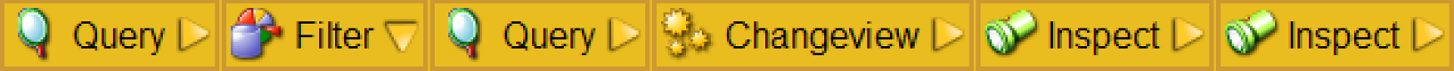
\includegraphics[width=.8\columnwidth]{action-1}}

\vspace{.5\baselineskip}

\subcaptionbox{Iconic actions connecting two visualization states. \is{Ma1999}\label{fig:lr-action-2}}{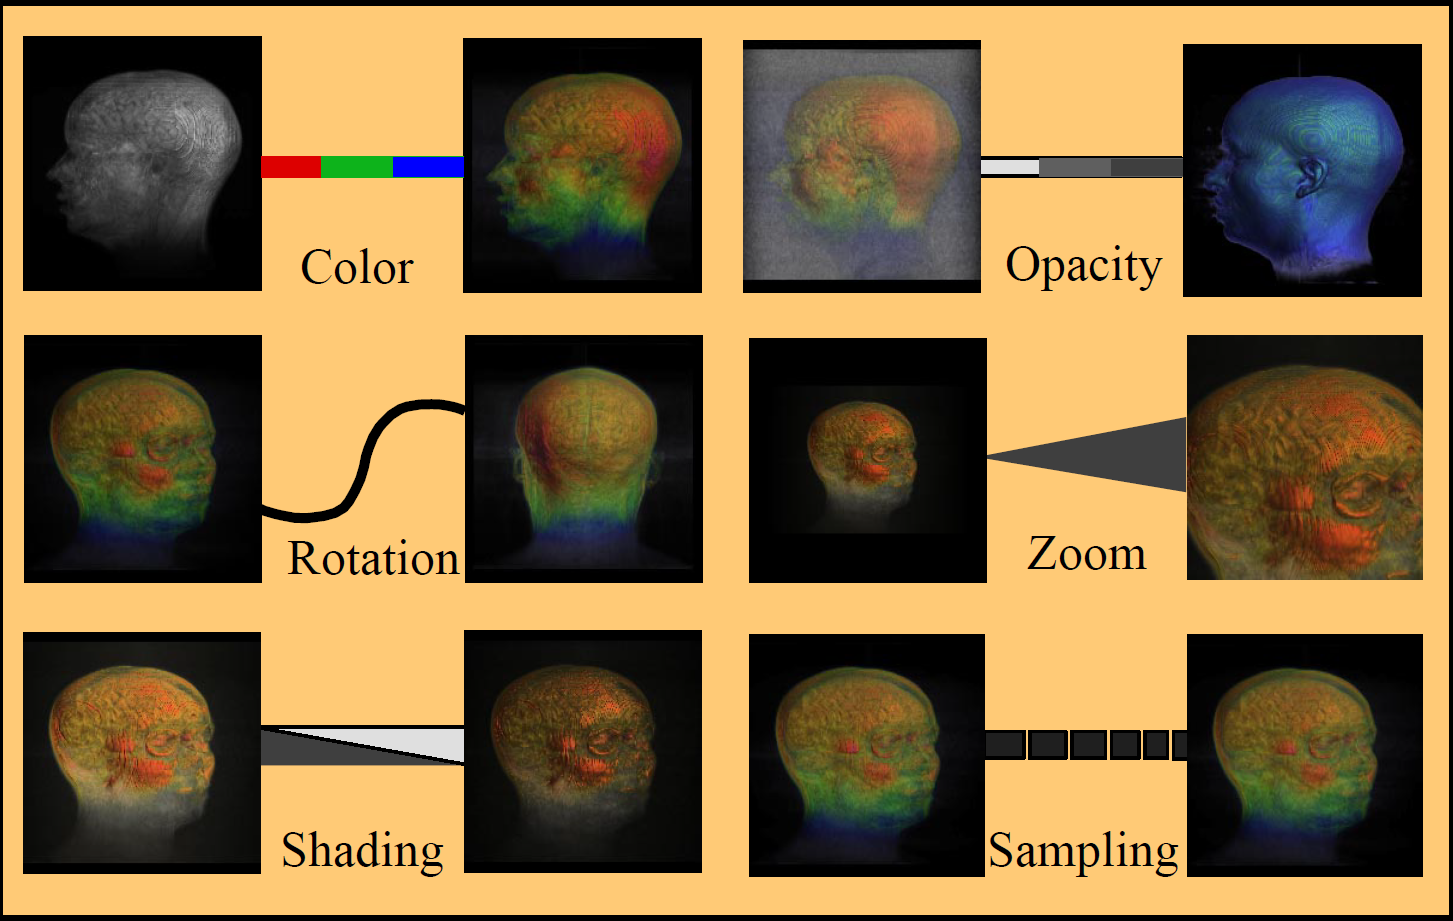
\includegraphics[width=.8\columnwidth]{action-2}}
\caption{Using icons for representing actions.}
\end{figure}


\paragraph{Thumbnail}
Thumbnails are commonly used to represent visualization states, aiding users' recognition of previous ones. One study suggests that a thumbnail size of 96 pixels square could provide 60\% accurate recognition of a visited web site~\cite{Kaasten2001}. For the same accuracy but in recognizing an exact web page, the thumbnail size rises to 144 pixels square. Additional information can be added to a web thumbnail to improve its recognition such as how often the represented page is revisited and whether that page is bookmarked or not~\cite{Cockburn1999}. For visualization thumbnails, visual encodings and parameters that were used to produce the visualization can also be embedded (\autoref{fig:lr-thumbnail-encoding}), providing more provenance information to the users.

\begin{figure}[!htb]
	\centering
	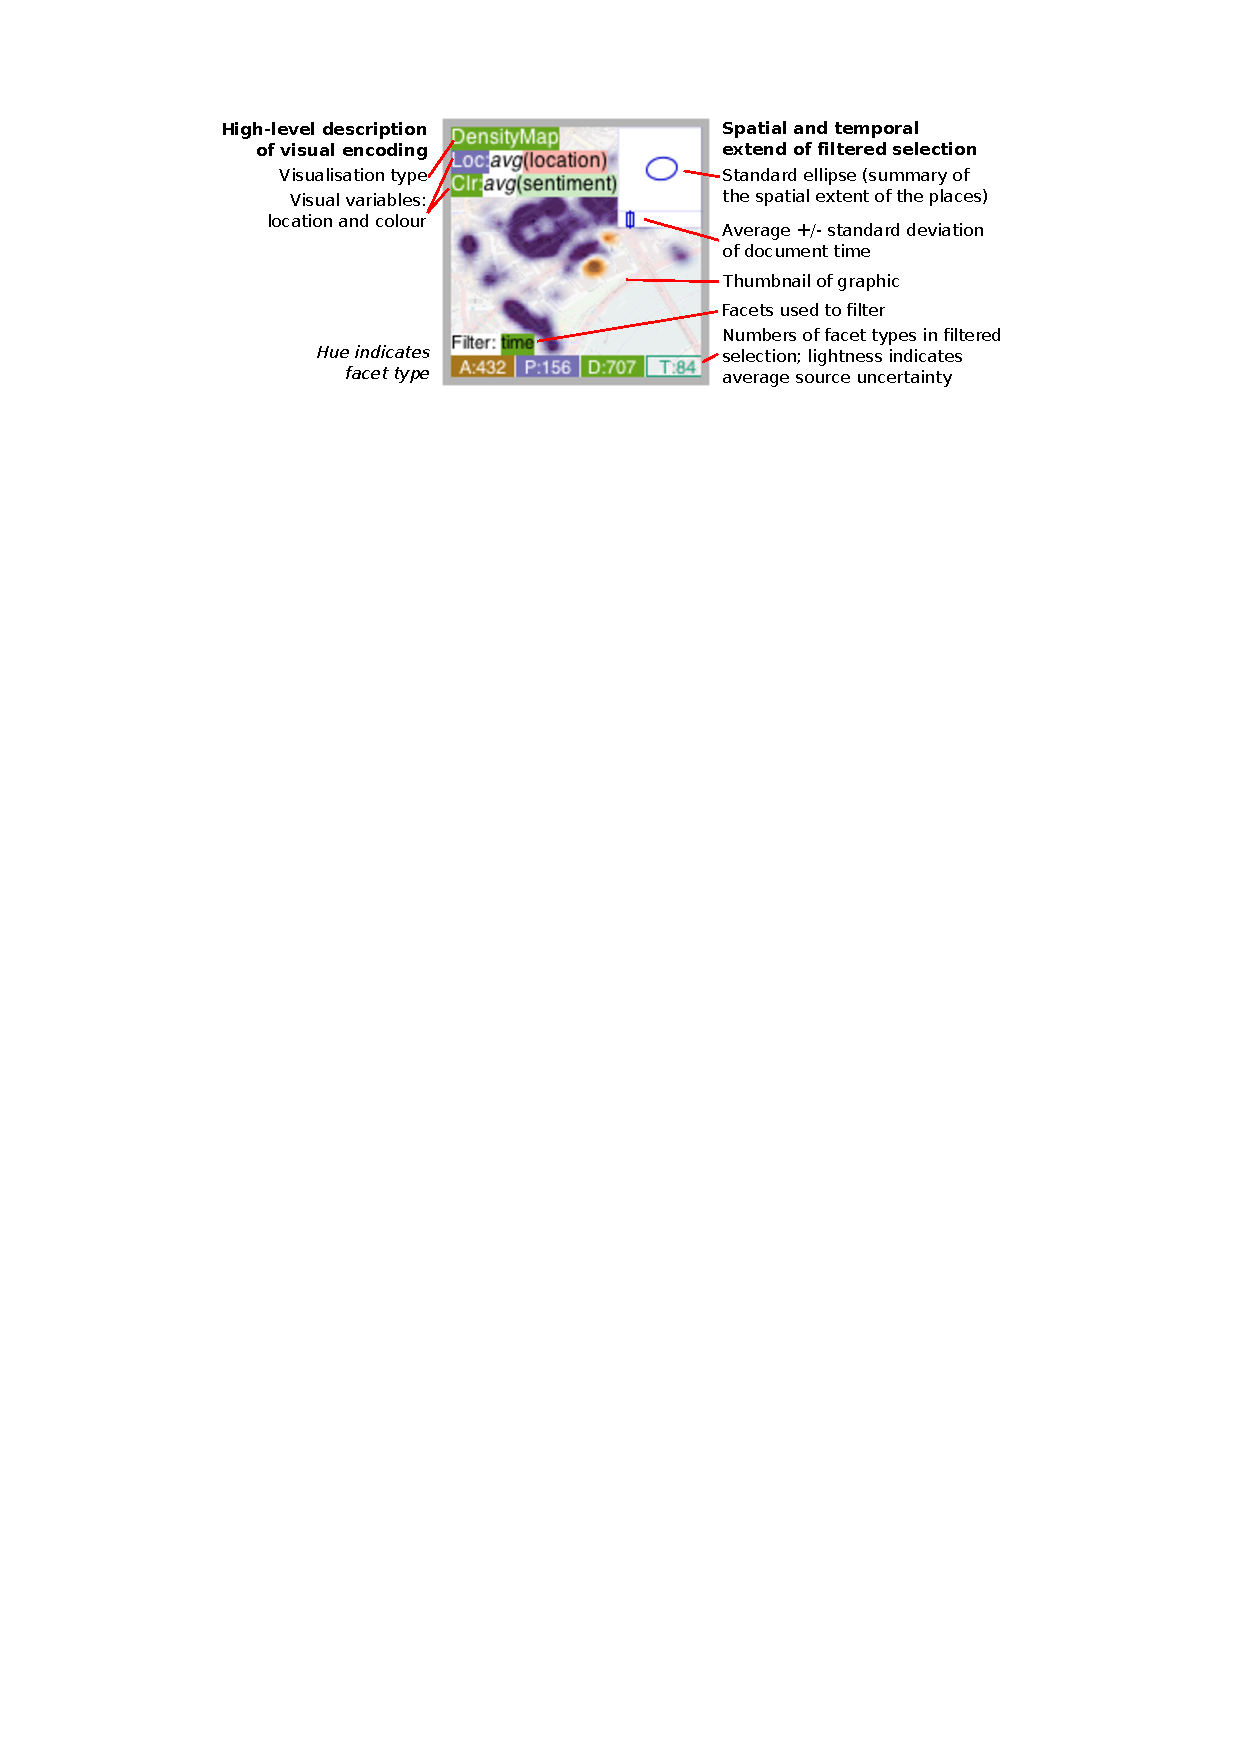
\includegraphics[width=\columnwidth]{thumbnail-encoding}
	\caption{Visualization thumbnails with additional information about any filtering used, the characteristics of the filtered subset of data and the visual encoding. \is{Walker2013}}
	\label{fig:lr-thumbnail-encoding}
\end{figure}

It may be necessary to apply pre- and post-processing adjustments to make the visualization thumbnails more recognizable~\cite{Heer2008}. For example, high-frequency visual elements that are not helpful in a small size such as gridlines and element borders can be removed to prevent their domination in the resulting thumbnail. As a result of down-sampling techniques, colors of data items may be different from them in the original visualization. Therefore, readjusting the color to match its intended value could help users to recognize the visualizations they analyzed in the past.

The default snapshot may also be an imperfect representation of a web page, especially if it contains a lot of text. Teevan~et~al.~\cite{Teevan2009} propose an automatic method to produce a thumbnail improving its recognition. It consists of three components: some salient text at the top-left hand corner, a salient image below the text, and a watermarked logo superimposed at the bottom left hand corner of the image. The salient text contains about 20 first characters of the web page title. The salient image and the branding logo are chosen from the page using machine learning. \autoref{fig:lr-enhanced-thumbnail} shows such a thumbnail.

\begin{figure}[!htb]
	\centering
	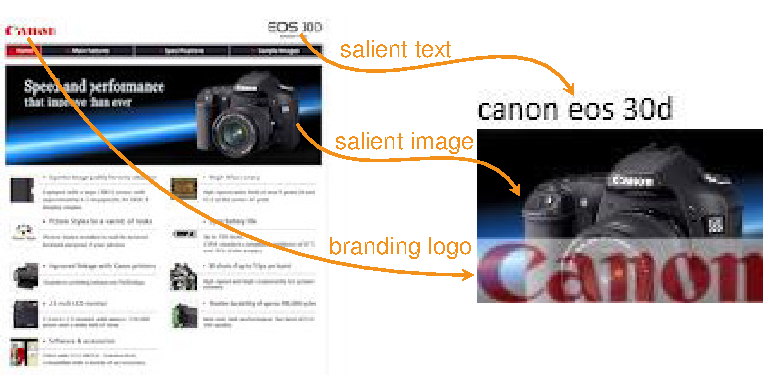
\includegraphics{enhanced-thumbnail}
	\caption{An enhanced web thumbnail (right) as a composite of some salient text, a salient image and a branding logo. \is{Teevan2009}}
	\label{fig:lr-enhanced-thumbnail}
\end{figure}

Besides recognizing previous states, seeing the difference between a state and the one before it is also important in understanding the analysis process. One approach is to highlight the difference between two consecutive states (\autoref{fig:lr-state-2}). The changes may only happen at one small portion of the entire interface. Therefore, showing only that area in both states could help users quickly identify the difference (\autoref{fig:lr-state-3}).

\begin{figure}[!htb]
\centering
\subcaptionbox{Modified items are highlighted with green borders. \is{Klemmer2002}\label{fig:lr-state-2}}[.47\columnwidth]{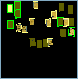
\includegraphics[height=.33\columnwidth]{state-2}} 
\hfill
\subcaptionbox{Changed area is cropped and shown in both  states. \is{Kurlander1988}\label{fig:lr-state-3}}[.47\columnwidth]{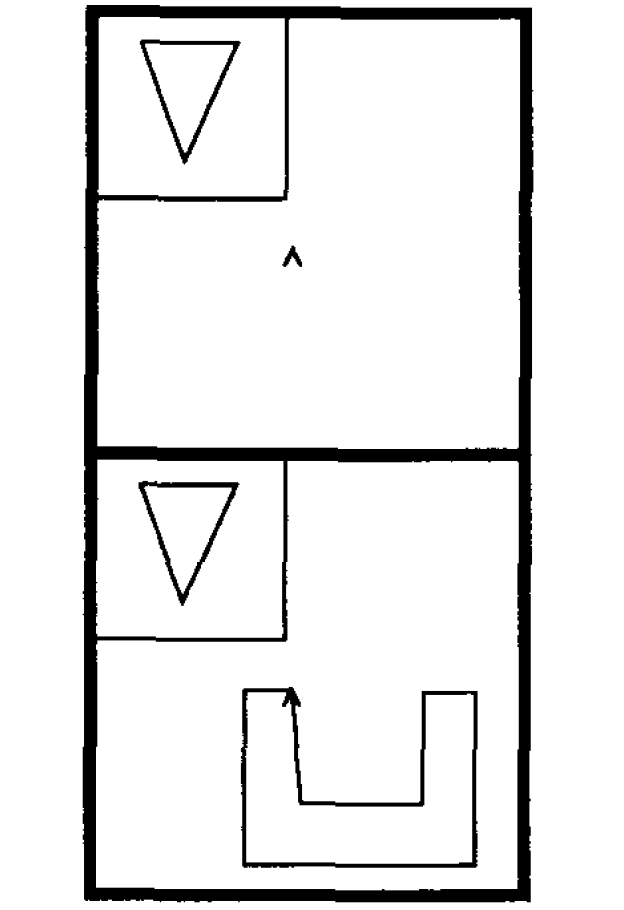
\includegraphics[height=.33\columnwidth]{state-3}}
\caption{Techniques improving recognition of state changes.}
\end{figure}

\subsubsection{Layout}

\paragraph{Linear Layout}
Provenance data usually contains an inherent \emph{time} attribute, recording when an action happened. An approach that emphasizes on the order of completed actions is to show them as a linear sequence of items like a comic strip~\cite{Kurlander1988,Meng1998}. This layout facilitates visual scanning of past actions, allowing users to quickly understand the analysis process. \autoref{fig:lr-comic-strip} shows such a layout.

\begin{figure}[!htb]
	\centering
	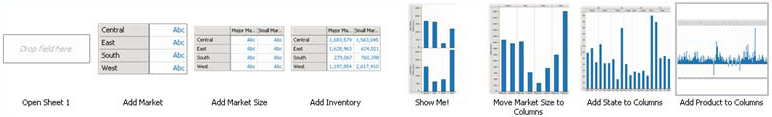
\includegraphics[width=\columnwidth]{comic-strip}
	\caption{Comic strip layout. A sequence of past actions in chronological order. \is{Heer2008}}
	\label{fig:lr-comic-strip}
\end{figure}

If the absolute timestamps of actions are of interest, a continuous timeline~\cite{Derthick2001} is a more suitable layout. Actions are positioned along the time axis at when they happen (\autoref{fig:lr-continuous-timeline-1}) or during which they last (\autoref{fig:lr-continuous-timeline-2}). The time axis can be either horizontal or vertical~\cite{SandboxTimeline2012}. The layout algorithms found in these provenance timelines are quite naive. POLESTAR~\cite{Pioch2006} and the timeline from Jigsaw~\cite{Liu2010} require manual rearrangement of the events from users to solve the overlapping problem. The timeline from nSpace2 Sandbox~\cite{SandboxTimeline2012} shows events at the exact time when they happen without considering possible intersection between of them.

\begin{figure}[!htb]
\centering
\subcaptionbox{Time-point provenance data. User annotations are positioned along a time axis at when their associated events happen. \is{Gotz2006}\label{fig:lr-continuous-timeline-1}}{\includegraphics[width=\columnwidth]{continuous-timeline-1}}

\vspace{.5\baselineskip}

\subcaptionbox{Interval provenance data. User actions are shown as horizontal bars a long a time axis covering their durations. \is{Plaisant1999}\label{fig:lr-continuous-timeline-2}}{\includegraphics[width=\columnwidth]{continuous-timeline-2}}
\caption{Timeline layout for visualizing the analysis process.}
\end{figure}

Another approach is to use both the horizontal and vertical axes to represent time. BrowseLine~\cite{Hoeber2009} uses the vertical axis for \emph{macro-time} and the horizontal axis for \emph{micro-time}, similar to stem-and-leaf plots. More specifically, a two-dimensional timeline (\autoref{fig:lr-timeline-2d}) is divided into rows, each for a big time-slot, such as one hour. In each row, events happening within that hour are positioned along the horizontal axis without considering their absolute timestamps. This design assumes that users may only remember roughly when events happen, thus absolute positioning in the vertical axis facilitate them in recognizing past events. Moreover, relative positioning in the horizontal axis could help pack more events and prevent overlapping.

\begin{figure}[!htb]
	\centering
	\includegraphics[width=\columnwidth]{timeline-2d}
	\caption{2D timeline. The vertical axis represents macro-time, whereas the horizontal axis represents micro-time. Events within a macro time-slot are positioned in chronological order as a comic strip. \is{Hoeber2009}}
	\label{fig:lr-timeline-2d}
\end{figure}

\paragraph{Branching Layout}
Many sensemaking systems allow users to revisit their past states such as through undo/redo features or backward/forward in web browsers. From a past state, if the user performs a new action, it should be recorded in a new branch forking from that state. This branching history is typically visualized with a tree layout to represent the logic of the analysis process effectively. In such a tree, nodes represent a summary of system states, and edges represent actions that transition the system from one state
to another. Examples can be found in provenance-enabled systems in different fields including scientific visualization~\cite{Ma1999}, information visualization~\cite{Dunne2012}, visual analytics~\cite{Kadivar2009} and browser history~\cite{Ayers1995}. \autoref{fig:lr-tree-prov} shows such a provenance tree.

\begin{figure}[!htb]
	\centering
	\includegraphics[width=.7\columnwidth]{tree}
	\caption{Tree visualization for branching analysis process. Nodes are thumbnails of past visualization states and links are transforming actions. \is{Jankun-Kelly2007}}
	\label{fig:lr-tree-prov}
\end{figure}

% Time encoding
In a tree layout, the order of actions can be inferred through the direction of edges. Moreover, exact time gap between actions can also be visually encoded into the visualization. VisTrails~\cite{Bavoil2005} color-codes the background of nodes according to their creation time (\autoref{fig:lr-tree-time-1}). Aruvi~\cite{Shrinivasan2008} uses the length of edges to represent the relative time gap between two states (\autoref{fig:lr-tree-time-2}). 

\begin{figure}[!htb]
\centering
\subcaptionbox{Node backgrounds are color coded based on time. \is{UniversityofUtah2012}\label{fig:lr-tree-time-1}}{\includegraphics[height=0.21\columnwidth]{tree-time-1}} 
\hfill
\subcaptionbox{The edge length between two nodes represents the interval between them. \is{Shrinivasan2008}\label{fig:lr-tree-time-2}}{\includegraphics[height=0.21\columnwidth]{tree-time-2}}
\caption{Encoding temporal information into provenance trees.}
\end{figure}

% Other variations
The diagonal arrangement of tree as in~\autoref{fig:lr-tree} may consume a lot of space. One approach is to use only horizontal and vertical edges as in~\autoref{fig:lr-tree-time-2}. Another approach is to display only the path that led to the currently active  visualization~\cite{Klemmer2002}. Other paths can be expanded on demand. \autoref{fig:lr-inline-history-2} shows examples of representations of the active path and the full history.

\begin{figure}[!htb]
\centering
\subcaptionbox{Branched history. The user first performed actions $A$, $B$, $C$, $D$ and $E$, then undone to $D$, $C$ and $B$, then performed new actions $F$ and $G$.  \label{fig:lr-inline-history-1}}{\includegraphics[height=.178\columnwidth]{inline-history-1}}
\hfill
\subcaptionbox{Inline branching history representation. Top: displaying the current path. Bottom: displaying the full history; actions not part of the current path are placed between brackets. \label{fig:lr-inline-history-2}}{\includegraphics[height=.188\columnwidth]{inline-history-2}}
\caption{Branching layout for tree visualization of the analysis process. \is{Klemmer2002}}
\end{figure}

% Interaction for scalability
Interaction is also commonly used to address the scalability issue. Zooming and panning allow users to see the overview of the analysis process and navigate to the part of interest~\cite{Dunne2012}. Collapsing and expanding branches of the tree on demand can also help reduce its size and avoid distraction~\cite{Bavoil2005}. Distortion techniques may help users to quickly navigate and focus on more relevant states and actions~\cite{Meng1998}. Another technique for compressing the provenance tree and improving user understanding is \emph{action chunking}~\cite{Heer2008}: a sequence of related actions may be better represented as a single higher-level action. For example, a quick succession of sort or filter actions likely indicate a multi-step configuration of the view and can be chunked together.

Typically, provenance data is shown in a separate view, linked with other data views of the visualization system~\cite{Shrinivasan2008,Heer2008,Pike2009,Kadivar2009}. However the system can also be used as a single item of the provenance view. For instance, in GraphTrail~\cite{Dunne2012} -- a single-view visualization system, when the visualization is changed (e.g., changing attribute mapping in a bar chart), it creates a new view containing that visualization and links with the current view. This is similar to how normally the provenance view is developed; however, GraphTrail makes the entire exploration space become the provenance view. Moreover, each history item is not a thumbnail, but a fully interactive visualization. By allowing zooming and panning, users can choose between a close examination of individual system states (\autoref{fig:lr-detail}) and an overview of the analysis structure (\autoref{fig:lr-overview}). An extra overview window as in overview-and-detail technique~\cite{Cockburn2008} could be useful in search and navigation in a large space.

\begin{figure}[!htb]
\centering
\subcaptionbox{Zooming in to work on the active visualization.\label{fig:lr-detail}}{\includegraphics[height=0.56\columnwidth]{GraphTrail-detail}} 
\hfill
\subcaptionbox{Zooming out to see an overview as the history of the exploration process.\label{fig:lr-overview}}{\includegraphics[height=0.56\columnwidth]{GraphTrail-overview}}
\caption{Unification of the exploration view and the history view. \is{Dunne2012}}
\end{figure}

\subsection{Visualizing the Reasoning Process}
The reasoning process reflects user findings, methods and strategies in performing a task. This process mainly happens in the user's mind, and some sensemaking systems allow the user to manually externalize it through user bookmark~\cite{Walker2013}, annotation~\cite{Heer2009}, and manipulation of those externalized items~\cite{Xu2014}. A common form of reasoning externalization is to allow the user to write down their thinking. It could be a free note~\cite{Shrinivasan2008} or a description of a user bookmarked visualization~\cite{Walker2013}. Alternatively, users can annotate directly on the visual bookmark using standard graphical editing features such as circling on interesting patterns (\autoref{fig:lr-annotation-1} -- Top) or hand drawing on a suspicious trend (\autoref{fig:lr-annotation-1} -- Bottom). To make the annotation meaningful across multiple views, the selection should be aware of the data involved in it~\cite{Heer2008a}. For example, in~ \autoref{fig:lr-annotation-2}, the annotation in the top view also makes the data items in the bottom view get annotated using the same selection query. Data-aware annotations allow users to see the data of interest remained across different views.

\begin{figure}[!htb]
\centering
\subcaptionbox{Geometric annotation.\label{fig:lr-annotation-1}}{\includegraphics[height=0.7\columnwidth]{annotation-1}} 
\hfill
\subcaptionbox{Data-aware annotation.\label{fig:lr-annotation-2}}{\includegraphics[height=0.7\columnwidth]{annotation-2}}
\caption{User annotation of bookmarked visualization.\is{Heer2012}}
\label{fig:lr-annotation}
\end{figure}

% Interaction
A note can simply be any user thought, but it can also take on different roles such as \emph{evidence}, \emph{assumption} and \emph{hypothesis}~\cite{Pike2009}. They have different visual representations, enabling users create and manage their complex reasoning processes. Typically, users are allowed to move notes freely and draw edges to connect them, enabling spatial grouping of related notes and relationships establishment. These interactive features are known to help users produce more critical thinking in their analyses~\cite{Sedig2013}. For example, users can show connections between a hypothesis and its evidence by drawing links, and spatially separate the evidence into a supporting group and a counter group, facilitating further comparison. \autoref{fig:lr-reasoning-simple-note} shows such a diagram produced with user notes and \autoref{fig:lr-reasoning-diagram-SRS} shows such a more formal diagram with different reasoning roles.

\begin{figure}[!htb]
\centering
\subcaptionbox{A diagram of user notes showing their thoughts. \is{Shrinivasan2008}\label{fig:lr-reasoning-simple-note}}{\includegraphics[height=0.42\columnwidth]{reasoning-simple-note}}
\hfill
\subcaptionbox{A formal reasoning diagram with nodes having different roles: evidence, casual relationship, assumption and hypothesis. \is{Pike2009a}\label{fig:lr-reasoning-diagram-SRS}}{\includegraphics[height=.42\columnwidth]{reasoning-diagram-SRS}}
\caption{Visualization of reasoning process.}
\end{figure}

% Formal reasoning
More analytical reasoning methods have also been applied on the provenance data. The SRS system~\cite{Pike2009} first allows the user to construct a reasoning diagram with bookmarked visualizations as evidence nodes and causal relationships as links (\autoref{fig:lr-reasoning-diagram-SRS}). These evidence nodes and links may lead to a hypothesis. The user then specifies their confidence about the evidence before the system computes the likelihood of the hypothesis using the Dempster–Shafer belief network~\cite{Sanfilippo2007}. The result provides analytical support to the user. 

POLESTAR~\cite{Pioch2006} supports argument structuring, based on methods for analyzing legal documents such as the Toulmin model of argument~\cite{Toulmin2003}. To help validate a hypothesis, it organizes arguments as a tree structure of claims, each supported by at least one piece of evidence. A claim can have its supporting sub-claims and can also have rebuttals that weaken or restrict their force. \autoref{fig:lr-reasoning-argument-editor} shows such a argument tree. Sandbox~\cite{Wright2006} supports analysis of competing hypotheses -- a judgment method that requires careful weighing of alternative explanations~\cite{Heuer1999}. It allows users to add multiple hypotheses, each with supporting or contradictory evidence. These pieces evidence are weighted by the users and summarized in a visual matrix, enabling the users to effectively make a decision without having to remember and analyze in their minds. \autoref{fig:lr-reasoning-ACH} shows an example of this support.

\begin{figure}[!htb]
\centering
\subcaptionbox{Argument tree. Analysts elaborate arguments via a tree structure of claims, sub-claims, and facts. \is{Pioch2006}\label{fig:lr-reasoning-argument-editor}}{\includegraphics[height=0.3\columnwidth]{reasoning-argument-editor}}
\hfill
\subcaptionbox{Analysis of competing hypotheses. The interface allows adding multiple hypotheses, each with weighted supporting/counter evidence, and producing a summary matrix to evaluate them. \emph{\textrm{Image source: a video snapshot of~\cite{Wright2006}.}}\label{fig:lr-reasoning-ACH}}{\includegraphics[height=0.3\columnwidth]{reasoning-ACH}}
\caption{Analytical support for the reasoning process.}
\label{fig:lr-reasoning}
\end{figure}

%\chapter{Literature Review}

\graphicspath{{Chapter2/figures/}}

- sensemaking
 - some definitions of sm in different contexts
 - PCM
 - DFM
 
- visualization
- analytic provenance
 - capture
 - visualize
 - use
- challenges, gaps in the literature and we're addressing them in this thesis.



 
 \section{Sensemaking}
 Sensemaking is described as the process of comprehension, finding meaning and gaining insight from information, producing new knowledge and informing further action. It has been studied in different contexts such as human-computer interaction~\cite{Russell1993}, information science~\cite{Dervin1983}, and organizational studies~\cite{Weick1995}. Pirolli and Card offer a notional model of sensemaking~\cite{Pirolli2005}, describing a cyclic process involving searching and extracting information, representing it in schemata, manipulating the schemas to form and test hypotheses, then presenting the outcome. Klein et al.~\cite{Klein2006} offer a \textit{data--frame} model describing the interaction of data -- the aspects of the world, and frames -- the accounts of the ``sensemaker'' for the situation. The model consists of a few interconnected iterative processes, each for a certain type of sensemaking activity such as fitting data into a frame.

The notion of sensemaking relates to the way in which human process and interpret information about the world, leading to the creation of new knowledge or insight, which informs further action ~\cite{Pirolli2005}. There are a number of different sensemaking theories, which draw attention from scholars in human-computer interaction, psychology and other areas that consider sensemaking in different contexts. Examples include Dervin~\cite{Dervin1983}, who considers how sensemaking is related to information seeking behaviors and needs, and Weick~\cite{Weick1995}, who was concerned with how sensemaking takes place in organizational settings, from individual and social contexts. Pirolli and Card~\cite{Pirolli2005} offer a notional model of sensemaking, describing a cyclic process involving representations of information in \textit{schemata} and the manipulation of \textit{schemas} to gain insight forming some knowledge or understanding. Klein et al.~\cite{Klein2006} offer the \textit{Data/Frame} theory describing the interaction of \textit{data}, which are aspects of the world and \textit{frames}, that are the sensemaker’s representations of the situation. 

\section{Visualization}
\section{Analytic Provenance}

%\subsection{Timeline Visualization}
% Timeline visualization
%Timeline is one of the earliest visualizations. Back in 1765, Joseph Priestley created the Chart of Biography about two thousand famous people from 1200 B.C to 1750 A.D~\cite{Priestley1765} -- one of the oldest documented timeline. Along a horizontal timeline, Priestley used bars to depict lifespans and dots to illustrate the uncertain birth and dead dates. This remains one of the most popular visual metaphors for timeline visualization: time is represented as a horizontal axis; an event is plotted as a point if it is an instant or a bar spans its interval otherwise. Geographical information can also be included in timeline visualizations as in the classic information visualization example of Napoleon's March on Moscow in 1812-1813 by Charles Joseph Minard~\cite{Minard1869}. 

In this section, we consider related work on representing temporal data and producing timelines, before also examining larger visual analytic systems that include timelines in their feature set.

\subsection{Timeline Visualizations}
% Some examples based on timeline metaphor. Aggregate methods.
A typical example of timeline visualizations is LifeLines~\cite{Plaisant1996a}, a visualization for personal histories, which uses icons to indicate discrete events and thick horizontal lines for continuous ones. When the number of data items is large, they need to be shown collectively rather than individually. The river metaphor~\cite{Havre2002} is one such method that represents thematic changes in large document collections. Storyline visualizations illustrate the dynamic relationships between entities in a story. The technique was first introduced by Munroe with his hand-drawn visualizations~\cite{Munroe2009}. The visualization summarizes movie plots by depicting each character as a line and each interaction between characters as a converging or diverging bundle of those character lines. Computational layouts have since been introduced to automate the rendering process including work by Tanahashi and Ma~\cite{Tanahashi2012} and Liu et al.~\cite{Liu2013}. 

%There are other metaphors to represent temporal data such as the three-dimensional histogram~\cite{Kosara2004}, the spiral graph~\cite{Weber2001}, or calendar-based approaches~\cite{VanWijk1999}. More detail about timelines or more general time-oriented data visualizations can be found in the comprehensive work of Aigner et al.~\cite{Aigner2011}.

% Skip scalability issue because it's not addressed in SchemaLine
%While the time axis metaphor is simple and intuitive, it can be challenging to visualize a large number of events and the relationships among them along a timeline. In the simplest case, all events are unrelated and visualized independently on the timeline. When several events happened during a short period, multiple layers above the timeline need to created to ensure each event's position matches its time point and no two event descriptions overlap~\cite{Plaisant1998,Pioch2006,Andre2007,Liu2010,Kim2010,Munroe2013,SimileTimeline,TimeGlider}. \note[k]{We mentioned timeline scalability here and need to discuss it for SchemaLine} The resulting timeline can quickly get cluttered as events and layers increase. Several attempts have been made to address the scalability issue including semantics zooming with different levels of detail \cite{Andre2007}, focus and context views \cite{Andre2007, SimileTimeline}, and aggregation of multiple events to one single event \cite{Plaisant1998}.

% Visualize relationships between events
Visualizing individual events on a timeline is relatively simple; however, showing relationships between events is quite challenging. One approach is to explicitly draw an edge between two related entities as in tmViewer~\cite{Kumar1998}. Edge styles can be used to depict different kinds of relationships; however, drawing a node-link diagram on top of the timeline can cause the visualization to become cluttered even with a small number of events. Another method is to use the concurrent perception ability of humans by using color coding or icons to indicate different groupings. When events are distributed along the timeline, this method introduces a heavy cognitive load for viewers to scan through the entire timespan. Our method uses colored backgrounds and clusters all events belonging to the same group to reduce user effort. Relationships within multiple faceted temporal data are addressed by Andr\'{e} et al. in Continuum~\cite{Andre2007} by using views with different scales and the classic details-on-demand technique to save space. More recently, SemaTime~\cite{Stab2010} can visualize two different types of relationship: time-dependent (e.g., lives-in) and time-independent (e.g., father-of). SemaTime stacks events vertically and places related events close together. Time-dependent relationships are depicted by using rectangles crossing the relevant common interval of the two events. Time-independent relationships are illustrated by simple arrows.

% Follow events in timeline
%One essential requirement in timeline visualizations is to be able to follow events chronologically. Even though events are aligned with their time, it can still be difficult to trace which events happen after which, especially when they are close. A conventional rule is that an event is preferentially rendered at the bottom. If the representation of the event (normally a short summary of the event) does not overlap with other event representations, it will stay at the bottom; otherwise, it needs to move up a level. In place of this implicit rule, our method creates an explicit path to guide readers, to improve performance in both time and accuracy. 

%Visual attributes, such as colors and font sizes, are commonly used when events have other attributes (such as grouping and importance level) need to be included in the visualization \cite{TimeGlider}. \note[k]{Similarly, we mentioned number of distinguishable colour issue here and need to discuss it for SchemaLine} However, the number of colors that can be easily distinguished is limited, and so are the levels of possible font sizes to ensure legibility and not taking up too much display estate. 

%To address these problems, LifeLines \cite{Plaisant1998} divides the vertical dimension of timeline into multiple stacks, each to represent a group of events. Continuum \cite{Andre2007} represents the hierarchical relationships between events by displaying child events nested in a parent event. For example, in the music context, a piece belongs to a composer, a composer then lives in an era. All pieces of one composer can be displayed inside a bar of the composer, which represents his/her lifespan.

%Events can have additional complex relationships. In genealogical data, there are relationships such as marriage/divorce and parent-child. \note[k]{can reduce the details about this work if need space}{Kim et al. \cite{Kim2010} represent people as individual lines that cover their lifespans. Vertical axis is used to represent relationships. Unrelated people are displayed vertically far enough to indicate that there is no relationship between them. When two persons get married, the two corresponding lines converge into a bundle to indicate a marriage. Whereas, the diverge of a bundle of two lines denote a divorce. The child is visualized close to the bundle of his parents and a vertical faded dash-line is used to connect the beginning of the child line to his parents.} 

%Another example is movie data, in which a scene contains a start time, a duration and members involved. Munroe creates a hand-drawn visualization to summarize characters' interactions in movies, published in the XKCD webcomic ``Movie Narrative Charts'' \cite{Munroe2013}. Inspired from that work, Tanahashi and Ma~\cite{Tanahashi2012} propose a set of design considerations for aesthetic and legible story-line visualizations, and an algorithm to generate visualizations satisfying these design principles. Similar to representing marriage/divorce relationship in genealogical data,  character lines should go straight unless they converge to or diverge from an interaction. The bundle of lines in an interaction should be adjacent; otherwise, lines must be not adjacent to depict separate character lines. To improve the aesthetics and legibility of the visualization, the algorithm also tries to minimize the number of line wiggles (bends), line crossovers, and white space gaps. The visual representation of SchemaLine is inspired by this work. 

%\subsection{Narrative Construction}
%\label{sec:narrative}
%Segel and Heer \cite{Segel2010} reviewed and classified narrative visualizations based on three dimensions: genre, visual narrative tactics, and narrative structure tactics. They define seven (not mutually exclusive) genres of narrative visualizations including magazine style, annotated chart, partitioned poster, flow chart, comic strip, live show, and film/video/animation. Narrative visualizations can also be classified as author-driven, reader-driven, or hybrid. They give an example of a common approach called "Martini Glass Structure". The story begins with the author's guidance for a while and then leads to the reader-driven stage where they can freely explore the story. Among these, most relevant to our work are those designed for sensemaking and utilize a timeline representation.

\subsection{Timelines within Visual Analytics Systems}
A timeline is commonly integrated into Visual Analytics systems designed for making sense of large and complex datasets including POLESTAR~\cite{Pioch2006}, HARVEST~\cite{Gotz2006}, Jigsaw~\cite{Stasko2007, Gorg2013}, and nSpace2 Sandbox~\cite{Wright2006, SandboxTimeline2012}. 

% visualize what?
To support sensemaking, timelines are typically used to visualize not raw data, but more meaningful information such as user notes (POLESTAR, HARVEST) or extracted entities (Jigsaw, nSpace2 Sandbox) instead. HARVEST visualizes both raw data and synthesized knowledge in one timeline to allow progressive investigation. However, filtering must be supported to prevent valuable information getting lost among dense data.

% manipulation of notes
Most of the systems use timelines to show notes statically, to present a known story instead of dynamically discovering a hidden story. nSpace2 Sandbox is an exception -- it allows users to group related entities into sub-timelines and to alter the entity's date on the timeline if needed. However, one entity cannot be added into multiple timelines, which is necessary when an entity's category is uncertain. Our SchemaLine provides a set of fluid interactions to manipulate notes to build a more semantic schema.

% visual representation of notes and schemata
Notes are typically represented using the ``sticky-notes'' metaphor: a colored rectangle as background with text on top of it. nSpace2 Sandbox provides multiple levels of detail for entities: a short summary, a full article, or even entities of entities. Timelines are commonly visualized as a horizontal axis with notes connecting to the timeline by edges. nSpace2 Sandbox uses a vertical axis timeline as the ``diary'' metaphor with columns for sub-timelines.

% layout
POLESTAR requires manual notes arrangement to fit the display. nSpace2 Sandbox uses a simple linear layout to organize entities, thus entities with nearby dates will overlap on the timeline. Our layout algorithm produces an aesthetically pleasing visualization that avoids this issue while still providing easy note manipulation.

% integration
Timelines are often used as an extra view, coordinated with the whole system. Jigsaw provides a reasoning space called Tablet, where a timeline can be added. nSpace2 Sandbox also introduces a separate component called Timeline view. Even though entities from data space can be dropped into timeline space, it may introduce a heavy cognitive load for users to switch between two working spaces. In the evaluation of this paper, we integrate SchemaLine into an existing system seamlessly to provide concurrent exploration and sensemaking with data.

%is a collaborative knowledge management and sense-making tool for intelligence analysts. Users can extract text and take notes when reading documents. Notes are then placed in an empty space to allow analysts to organize and cluster information. This information can be organized in a timeline; however, the user needs to arrange it manually. Without automatic layout and grouping of related information, it is difficult to assist users in sensemaking.
%
%\note[p]{miss 1,3,4}
%HARVEST~\cite{Gotz2006} allows users to interactively define new knowledge when analyzing data. The synthesized information can then be visualized together with raw data on the timeline. This feature could be useful because insight can be progressively used to gain deeper understanding. However, it may cause the findings get lost among dense data; only selective information should be shown on the timeline. The system does not support linking or grouping synthesized knowledge to produce alternative explanations about the case.
%
%\note[p]{miss 3,4,5}
%Jigsaw~\cite{Stasko2007} is one of the most popular Visual Analytics systems for making sense of a large corpus of documents. It can identify various types of entity (people, place, organizations, etc.) within the corpus and present the complex relationships through multiple linked visualizations. Jigsaw also supports a timeline for sensemaking~\cite{Gorg2013} within a feature called ``tablet''. Tablet is an empty canvas, which allows analysts to freely organize information, create links between entities or take notes. When entities are dropped onto the timeline, they will be automatically organized based on their associated date. A disadvantage of the tablet is that the user needs to open another space to enter notes instead of directly inside the data exploration space. The tablet timeline does not support visually showing different groups of related notes, which is quite important when connecting them together to construct a more cohesive explanation. It is also not clear how this timeline is used to support analysis; it is more often used for reporting the story once discovered~\cite{Liu2010}.
%
%\note[p]{miss nothing!!!} \note{maybe we can say how schemaline is different instead?}
%nSpace Sandbox~\cite{Wright2006} is a commercial sensemaking environment that supports extracting information from different sources, organizing it flexibly and linking these pieces of information. Sandbox's timeline~\cite{SandboxTimeline2012} allows the assembly of different types of evidence, such as documents or pictures, along the time axis. It also supports creating \textit{bands} within the timeline to store different groups of events. Relationships between events within bands or within the timeline are visualized by arrows. Sandbox's timeline is quite advanced in terms of analytical features compared to the timelines in other visual analytics systems. However, the simplistic linear timeline layout is not space-efficient and also makes it difficult to visualize close events. Zooming feature is provided to partially address this issue.

%Visualizing documents along a timeline is one of its many features, but it does not directly support group or interactive editing.
%\note[k]{this needs to be updated for later/latest version of GeoTime. Also the focus should be 'timeline' and not 'narrative'} GeoTime \cite{SandboxTimeline2013} is a Visual Analytics system that is designed for the detection of spatial and temporal pattern within the data. It allows annotated visualizations, which can then be used to build a visual narrative. However, the visual narrative is mainly designed for reporting, and there is limited functionalities for the discovery process of the narratives.
%Aruvi~\cite{Shrinivasan2008} is a Visual Analytics system designed to support sensemaking. It allows the creation of notes about any finding and the visualization leads to it. Such notes can be connected to indicate the relationship between them. However, it only provide free-form organization of the notes and there is no support for timeline visualization. 
%HARVEST \cite{Shrinivasan2009} is a Visual Analytics system that adopts a similar approach to sensemaking as the Aruvi. While it uses an algorithm to find relevant discoveries and views for suggestion, there is no significant changes in the support of sensemaking. As a result, it lacks the ability to automatically layout the finding notes or the support for the discovery of any temporal pattern.
%\note[k]{Phong, can you say something about the timeline in 'Sense.us'?} Sense.us \cite{Heer2009} is one of the early attempts of online collaborative visualization. It allows users to annotate visualizations and use them in the collaborative discussion. The trail of annotated visualizations are then used to construct the trail of a topic. This method is useful to record the evolution of the discussions, but it does not indicate the relationships among the discussion, i.e., how they form a narrative, and can make it difficult to understand a large discussion.
\note[p]{I have no idea with timeline in 'i2 analyst notebook'}






\section{Related Work}

\subsection{Timeline Visualizations}
The most common form of timeline visualization uses a horizontal axis to represent time progressing from left to right, with events positioned horizontally according to their timestamps. A well known example is LifeLines~\cite{Plaisant1998} -- a visualization of personal medical records. LifeLines uses icons to indicate discrete events and thick horizontal lines for continuous ones. Timelines can be integrated into a tree format to represent changes in a hierarchy over time as in TimeTree~\cite{Card2006}. Geographical information can also be embedded in timelines as in the classic visualization of Napoleon's March in Moscow in 1812--1813 by Charles Joseph Minard~\cite{Minard1869}. The book by Aigner et al.~\cite{Aigner2011} provides a comprehensive review of timelines and other time-oriented data visualizations.

Techniques such as aggregation and interaction are commonly used when there are a large number of events. LifeLines~\cite{Plaisant1998} aggregates events to save display estate; for example, a series of similar prescriptions can be grouped together. ThemeRiver~\cite{Havre2002} or Streamgraph~\cite{Byron2008} uses a river metaphor to represent aggregated changes of themes over time in a large document collection. Each river is a theme, and its width at certain time points shows the number of documents in that theme. Common interaction techniques are often used in the visualization of large timelines to support their exploration, including overview+detail \cite{Andre2007},  filtering~\cite{Plaisant1996a}, and details-on-demand~\cite{Stab2010}.

\subsection{Set Relations in Timelines}
According to the Gestalt principles of grouping, humans naturally perceive objects as a whole rather than as the sum of their parts~\cite{Koffka1935}. Three of the principles are commonly used to show set relationships among events: similarity, proximity, and uniform connectedness.

The principle of \textit{similarity} states that objects are perceptually grouped together if they are similar to each other~\cite{Koffka1935}. This principle is extensively applied to show set relations in timelines by using colors and shapes. Time indicators as icons (time-point events)~\cite{SimileTimeline2009} and bars (interval events)~\cite{Wang2008} are colored according to event set memberships. Different shapes for icons~\cite{TimeGlider2012} and bars~\cite{Plaisant1998} are also used to distinguish set memberships. It is more challenging to represent multiple set memberships. LineSets~\cite{Alper2011} uses concentric circles for icons, where each circle is colored to represent one set.

According to the \textit{proximity} principle, objects that are close together are perceived to be more related than objects that are spaced further apart~\cite{Koffka1935}. In Chart of Biography~\cite{Priestley1765}, people within a category are placed in a horizontal band, away from people in other categories. LifeLines~\cite{Plaisant1998} splits medical records into different sets, such as \textit{medication} or \textit{diagnosis}, and places them into vertically stacks, which works well if no two sets overlap. Storyline visualizations~\cite{Tanahashi2012,Liu2013} use curved lines to show interactions among characters within the movie timeline. Character lines converge to a bundle if they appear in the same interaction, and diverge when the it ends. Each line can be considered as a set passing through all of its members, and each interaction is a multi-set event. Thus, this method only works for interval events.

Elements tend to be grouped together if they are visually connected~\cite{Palmer1994}. Following this \textit{uniform connectedness} principle, SchemaLine~\cite{Nguyen2014} draws a rectilinear path connecting events belonging to a same set together. Also, tmViewer~\cite{Kumar1998} links related entities with line segments. Different line colors, thicknesses, and styles were used to distinguish set relations. This method can show events with multiple set memberships by connecting them with multiple edges. However, extra edges and crossings may negatively impact the readability of the timeline.

When similarity and proximity are applied together, the later principle dominates~\cite{Ware2013}. Moreover, uniform connectedness is stronger than proximity~\cite{Palmer1994}. For example, objects with different colors and shapes but located close together are more likely to be perceived as a group, and distant objects but with a closed contour surrounding them also provide a strong sense of grouping. Applying these ideas to visualize set relations for timelines, methods relying on similarity such as colored icons~\cite{Wang2008} are less effective than spatial grouping methods such as LifeLines~\cite{Plaisant1996a}. And those, in turn, are less effective than methods using line segments such as tmViewer~\cite{Kumar1998}. 

\subsection{Set Visualizations}
Sets and their relationships can be visualized using Venn~\cite{Ruskey1997} or Euler~\cite{Rodgers2014} diagrams. Simonetto et al.~\cite{Simonetto2009} proposed a technique to automatically visualize sets that were previously not possible with Euler diagrams. However, the complex shapes it produces may reduce visualization readability. In their controlled study, Riche and Dwyer~\cite{Riche2010} showed that for complex set intersections, duplications of shared elements resulted in a better performance in readability tasks than a none-duplicated visualization with more complex shapes. 

These methods assume the positions of set elements are not fixed, which reduces their applicability for geo-located or timeline events. Techniques without such constraints include Bubble Sets~\cite{Collins2009a}, LineSets~\cite{Alper2011}, and KelpFusion~\cite{Meulemans2013}. These methods employ the connectedness principle of the Gestalt laws~\cite{Palmer1994} by connecting set elements using extra visual elements. Bubble Sets draws an iso-contour surrounding elements within a set. This iso-contour is filled with a semi-transparent color so that the intersection between sets is shown as an area of blended color. Collins et al.~\cite{Collins2009a} provided an example of applying Bubble Sets to a timeline, in which case a force-directed algorithm is used to adjust the vertical positions of elements while the horizontal position along the time axis is fixed. 

LineSets applies a B\'{e}zier curve to connect data items. The curve follows the shortest path passing through all elements in the set. Its study showed that LineSets outperforms Bubble Sets in certain readability tasks ~\cite{Alper2011}. KelpFusion, a hybrid technique, uses lines for data-sparse areas and surfaces for data-dense areas. The results of an evaluation on readability tasks~\cite{Meulemans2013} demonstrated that it outperforms Bubble Sets in both accuracy and completion time, and outperforms LineSets in completion time. There has been no reported attempt to apply LineSets or KelpFusion to timeline visualizations. It is expected that crossings between lines, areas and the event text may reduce the timeline readability.







\section{Related Work}

\subsection{Sensemaking and Qualitative Analysis}
Qualitative research methodologies~\cite{adams2008qualititative} are commonly used in study of sensemaking. They allow researchers to reveal often complex user experiences and understand issues that are experienced subjectively or collectively~\cite{Pace2004327, adams2008qualititative}. Moreover, sensemaking research is often concerned not with testing an existing theory, but building a new one through the collection and analysis of relevant data, generating new knowledge about users and the usage of technology~\cite{rogers2012hci}.

There are a number of inductive approaches to qualitative research popular in sensemaking studies, such as \textit{grounded theory}~\cite{corbin1994grounded}, \textit{content analysis}~\cite{stemler2001overview}, and \textit{thematic analysis}~\cite{guest2011applied} that rely on the interpretation of rich textual and multimedia data. There is commonality in these approaches in that they all require a level of manual processing of data, coding and indexing it before describing it in the context of categories or themes. Furthermore, in the case of multimedia data, transcription of audio or video data is often also required. Though these approaches lead to important insights, they are labor intensive, time-consuming and costly in their application \cite{wong2002analysing}. There are a number of widely used software packages which are designed for researches using an inductive approach, offering ways to code and index data in various formats \cite{lewins2007using}. These tools give qualitative researchers useful ways of managing data, however, a qualitative analysis is still a largely manual process which requires a substantial investment of time and resources in leading to insightful findings.

\subsection{Analytic Provenance for Sensemaking}
Analytic provenance describes the interactive data exploration using a visual analytics system and the human sensemaking during that process. Besides the four semantic layers~\cite{Gotz2009} discussed earlier, it also includes the \textit{7W information}~\cite{provenance-7w} (Who, What, Where, Why, When,
Which, and hoW), which were initially proposed for \emph{data provenance}~\cite{data-provenance-survey-sigmod,data-provenance-survey-acm, data-provenance-survey-2008} that focuses on the data collection and computational analysis. This provides the context necessary for interpretation, such as authors, creation time, input data, and visualization parameters. Similar to other scientific workflows, an analytic provenance pipeline consists of capture, storage, analysis and visualization. Heer et al.~\cite{Heer2008} discussed design considerations for such pipeline, which covers underlying provenance's models, visual representations, and operations for analysis. The following discussions focus on the capture and visualization, in the context of recovering of user's sensemaking process from analytic provenance.

\subsubsection{Capture}
There is limited literature on capturing \emph{events} because it is relatively easy and provides little semantics alone. Among these, Glass Box~\cite{Cowley2006} can record a wide range of low-level \textit{events} such as mouse clicks, key strokes, and window events. Its objective is to capture and archive intelligence analysis activities so they can be retrieved later. On a higher semantic level, \textit{Actions}, such as changing the visualization settings and sorting a dataset, are usually performed through interactive widgets including menus and buttons. In theory, it is straightforward to capture them if a visualization system intends to do so. Some systems~\cite{Shrinivasan2008} maintain an action history to support undo and redo, which is an example of utilizing the actions' provenance.

Capturing \textit{task} and \textit{sub-task} is usually more challenging. As previously mentioned, such information is usually part of users' thinking that a visual analytics system does not have direct access to. Existing methods either take a manual or automatic approach. Manual approaches encourage users to record their thinking during sensemaking. However, this will not work if the method introduces considerable distraction or does not offer any benefits. Allowing user annotation is one of the most common forms~\cite{diva,schemaline}: the user creates \emph{notes} or \emph{annotations} that record comments, findings, or hypotheses. Those notes can be associated with the visualization, allowing users returning to the states when the notes were made~\cite{Pike2007, Shrinivasan2008} to re-examine the context or investigate further. The incentive to users is that such annotation digitizes a common sensemaking activity (i.e., note taking) and allows for features such as searching.  This also integrates notes with their visualisation context, allow for better interpretation. However, annotations are unlikely to cover all the analytical thinking. For example, users are more likely to record the findings they made than the process or approach that led them there. To encourage user to write richer notes, a visual analytic system needs to provide additional benefits such as the ability to create visual narratives~\cite{diva} that reveals the reasoning process and help users review and plan exploratory analysis for complex sensemaking task after recording the current progress~\cite{Lunzer2014}.

One of the main disadvantages of manual capture is the requirement of direct input from users. Automatic approaches try to address this by inferring higher level analytic provenance from what can be automatically captured including event and action provenance. However, this turns out to be a difficult task. An experiment studied the effectiveness of manual recovering of reasoning process from a user's action provenance, and the results showed that about 60\% to 70\% of high level analytic provenance can be correctly recovered~\cite{Dou2009}. Given the difficulty, a few methods attempted to partially uncover the high level analytic provenance. One such example is \textit{action chunking}, i.e., identify a group of actions that are likely to be part of the same sub-task, without knowing what the sub-task is~\cite{Gotz2009}. Such approaches apply heuristics to infer patterns from action logs based on repeated occurrence and proximity in data/visualization space or analysis time. More recently, there has been advancement in developing an automated and real-time technique to learn about users~\cite{Brown2014}. Based on very low-level events, mouse clicks and movements, collected from a visual search task, the algorithms can detect whether a user would be fast or slow at completing the task with 62\% to 83\% accuracy. They can also infer some user traits including locus of control, extraversion and neuroticism with 61\% to 67\% accuracy.

Deriving user thinking from their interaction data can be of value beyond understanding sensemaking and is common in other domains. For example, many websites record user browsing interactions in hope to derive higher level information such as user goals and needs. Data mining approaches are commonly used to detect patterns within such data~\cite{Cooley1997}, which can then be used to provide better service such as recommendations~\cite{Wei2007}. Chi et al.~\cite{Chi2001} proposed an algorithm to infer user needs from user's surfing patterns based on the concept of \textit{information scent}, which is the perception of the value and cost of information sources obtained from proximal cues with respect to the goal of the user~\cite{Pirolli1999}.

\subsubsection{Visualization}
Analytic provenance visualization is commonly used to provide an overview of the sensemaking process or reveal any patterns during this process, both of which can help researchers to understand users' thinking. Node-link diagrams are a popular choice to show an overview of the sensemaking process~\cite{vistrails,Pike2007,Shrinivasan2008,Kadivar2009,harvest,Dunne2012}. In most cases, nodes represent system states and edges are actions that transition the system from one state to another. Once an analytic provenance network is created, graph layout algorithms can be applied to improve the visualization. A sensemaking session can have hundreds of system states, and the analytic provenance network usually needs to share the display estate with other visualizations. As a result, it can be challenging to show the entire network within a limited space. It is possible to apply techniques for visualizing large networks such as clustering and aggregation. However, this needs to be done in a way that does not lose the information important for understanding the sensemaking process. To the best of our knowledge, we are not aware of any work addressing this challenge yet.

Besides the overall sensemaking process, the details of each system state and user actions are important for recovery of users' thinking. To provide more context, the common approach is \emph{detail on demand}: when a sensemaking step is selected, the visual analytics system shows the corresponding visualization state and the action's information ~\cite{Pike2007,Shrinivasan2008,Kadivar2009}. This works well if a visual analytics system allows user to go back to a previous state: showing the sensemaking context essentially restores all the visualization views to a previous state. However, to understand a sequence of sensemaking actions, researchers must go through one step at a time, sometimes back and forth. This can introduce extra cognitive work load on the user's memory, thus slow down the analysis. Methods such as GraphTrail~\cite{Dunne2012} show the full details of multiple system states and the links between them at the same time. By zooming and panning, users can choose to see more sensemaking steps (with less detail) or more information about individual system state (but less states simultaneously). This method works well when the visualization state is simple, e.g., only has one view. When a system consists of multiple visualizations, it becomes difficult to see the details of each state when more than one states are shown.

Chronicle~\cite{Grossman2010} utilizes a similar interface to SensePath, but with different design intentions. It captures the entire editing history of a graphical document to allow further study of how a complex image product is accomplished. In contrast, the goal of SensePath is to help analysts recover the high level sensemaking process. Following a similar approach, Delta~\cite{Kong2012} allows comparing different editing workflows to choose the most suitable one by visualizing the steps performed in those workflows. 



\section{Related Work}
Analytic provenance describes the interactive data exploration with a visual analytics system and the human sensemaking during that process~\cite{Xu2015}. Similar to scientific workflows, an analytic provenance pipeline consists of capture, storage, visualization and analysis~\cite{North2011}. Heer et al.~\cite{Heer2008} discuss design considerations for such a pipeline. The following discussions focus on the capture, visualization and utilization in the context of supporting sensemaking.

\subsection{Capture}
Gotz and Zhou~\cite{Gotz2009} divide analytic provenance into four layers according to its semantic richness (in descending order): task, sub-task, action and event. Capturing low level events is relatively straightforward but provides little semantics~\cite{Cowley2006}. Capturing provenance at ``action'' level is more common because it can be done automatically but still provides meaningful information~\cite{Shrinivasan2008, Nguyen2016}. However, capturing ``sub-task'' and ``task'' is more challenging because such information is usually part of users' thinking that systems do not have direct access to~\cite{Gotz2009,Xu2014}.

Brehmer and Munzner~\cite{Brehmer2013} provide a multi-level typology of abstract visualization tasks describing why the task is performed, how the task is
performed, and what are the task’s inputs and outputs. This typology breaks the intention of the user when performing actions into a three-level hierarchy, thus makes it more feasible to capture compared to the high level task and domain-dependent ``task'' and ``sub-task'' in the Gotz and Zhou's model.

% Web: What to collect which can support sensemaking
Information discovered during a browser-based sensemaking task can be collected at different levels of granularity: a web page URL~\cite{Baldonado1997,Gotz2007}, a page element such as \textit{table} and \textit{form} HTML tags~\cite{Schraefel2002,Hong2008}, or a specific fragment of text~\cite{Pioch2006,Nguyen2016}. Finer-grained capture allows users to record what they want with higher precision. Besides this manual capture, visited web pages can be recorded automatically as in browser's history feature. Page linking relationships among pages including opening from a web link and using browser's back button can also be captured~\cite{Ayers1995,Hightower1998,Milic-Frayling2003}.

% Web: Smart way to help collect more
% can remove to save space
%Several methods have developed to help users collect relevant information faster. SenseMaker~\cite{Baldonado1997} allows users to retrieve query results based on similarity with given examples such as web pages having the same domain or articles from co-authors. Dontcheva~et~al~\cite{Dontcheva2006} propose a method to extract similar information by first allowing users to collect a web element, then automatically extracting the information pieces having the same web structure as the collected sample. This method only works with web pages sharing the same template. \note[k]{I don't see any direct connection between sensemaker and Dontcheva's work and sensemap. They appear to be purely algorithmic.} ScratchPad~\cite{Gotz2007} computes and visualizes the relevance between the visiting web page and all the captured information, which may help the user determine the effort needs to spend on the web page.

% Cost structure paper: describe the study here
Besides what to capture, when to capture is also an important decision that needs to be made. Kittur et al~\cite{Kittur2013} conducted a user study to explore when is the best time to ask users to structure the captured information: when all the capture is done or at the same time with the capture. The results show that there are no significant difference between two options in terms of total time spent, cognitive workload, or preference. However, curation at a later stage has significantly better structured data because it has fewer dimensions and these dimensions have more commonalities across participants. 

%Kittur et al~\cite{Kittur2013} conducted a user study to characterize the costs and benefits of curation in the sensemaking process. More specifically, they compared two sensemaking strategies: curation completely after collection or curation at the same time with collection. \annote[k]{Information is collected by highlighting text and curated by assigning a dimension (i.e., tagging) and valence (good/neutral/bad). For instance, ``The Canon EOS Rebel T2i is \textit{good} in terms of \textit{lens}''}{this detail is not necessary}. The results show that there are no significant difference between two options in terms of total time spent, cognitive workload, or preference. However, curation later has significantly better structured data in terms of \annote[k]{fewer dimensions, fewer singleton dimensions, and more commonalities of dimensions across participants}{can you explain this without having to mention the details? It is not obvisou why 'fewer singleton dimensions' is better (or even what it is)}. \annote[k]{We wonder how a hybrid approach, let users curate whenever they want, would perform. We think that curating when collection is done may be adversely affected by the limit of users' working memory, especially with hourly length of sensemaking; and curating immediately after collecting a single piece of information loses the overall picture.}{move this to design discussion.}

\subsection{Visualization}
% Visualization
%In the simplest form, the collected information can be displayed as a list of items, each has a text showing the web page title~\cite{Schraefel2002}, or a table with rows for items and columns for attributes such as page title, URL and abstract~\cite{Baldonado1997}. Hunter--Gatherer~\cite{Schraefel2002} also provides a detailed view showing all collected information pieces together, each consists of a web page title, URL, and the actual captured web element such as text, form, image, and video.

%Tree is another option to organize collected information. SSGIS~\cite{Qu2003} can suggest an initial structure for the search results by clustering them into a tree. POLESTAR~\cite{Pioch2006} allows users to organize the collected snippets into a hierarchy and displays them as in ``Window Explorer''. Dontcheva~et~al~\cite{Dontcheva2006} present ``anchor-based'' layouts to display collected information pieces based on their common anchor attribute. For example, a \textit{calendar} layout can use to organize pieces based on their temporal information; and a \textit{map} layout is suitable to show their spatial information. Timeline is also a common metaphor to display temporal information~\cite{Pioch2006, Nguyen2015}.

Analytic provenance visualization is commonly used to provide an overview of the sensemaking process and to reveal any patterns during this process. Tree visualization is typically used for this purpose~\cite{Pike2007,Kadivar2009,Gotz2010,Dunne2012}. In most cases, a vertex represents a system state and an edge is an action transitioning one state to another. A branch indicates that the user revisits a state and performs another action. A long sensemaking session can produce hundreds of system states, thus makes it more challenging to show the entire process within a limited space. Large network visualization techniques such as clustering and aggregation can be applied to address this issue; however, this should not remove the important information for understanding the sensemaking process. Temporal information can be encoded either by color coded vertex~\cite{Bavoil2005} or edge length~\cite{Shrinivasan2008}. A timeline is also a common metaphor to display temporal information~\cite{Pioch2006, Nguyen2015}.

After understanding the overall sensemaking process, it is common to drill down to examine system states more in-depth. The common approach is \emph{detail on demand}: when a sensemaking step is selected, the visual analytics system allows the user to revisit that state~\cite{Pike2007,Shrinivasan2008,Kadivar2009}. Understanding a sequence of sensemaking actions is more difficult because it requires stepping through all of the actions, sometimes back and forth. This can introduce extra cognitive work load on the user's memory, thus slowing down the analysis. To address this issue, all states can be displayed at once as in Image Graph~\cite{Ma1999} and GraphTrail~\cite{Dunne2012}. However, it worsens the scalability issue.

\subsection{Utilization}
Analytic provenance supports visual narrative construction, during which the user composes findings into a cohesive story. A narrative can include provenance information at different levels: an analysis result, user notes, visualizations and raw data. DIVA~\cite{Walker2013} allows users to create a narrative based on user annotations and captured visualization states, and makes it possible to revisit the visualizations as when they were captured. SchemaLine~\cite{Nguyen2014} enables narrative construction grouping user notes along the timeline.

It is also possible to understand the sensemaking processes of other people by analyzing their analytic provenance~\cite{Dou2010}. SensePath~\cite{Nguyen2016} captures user sensemaking actions and provides a set of visualization and analysis tools allowing other people such as HCI researchers to explore the user sensemaking process through analysis of the captured actions.

% Tagging, node movement, links
%Captured information can be assigned labels or tags to attach meaning and then can be browsed and searched later~\cite{Hong2008, Ryder2010}. This could be a useful starting step in the curation process, which provides the user a semantic structure of the collected information. Other approaches allowing users to create relations among the collected pieces is to freely organize them in the display space~\cite{Pioch2006}  and to draw links connecting related pieces~\cite{Gotz2007}.

% Reasoning
To support further analysis, visual analytics systems commonly provide a ``reasoning workspace'', where the captured information can be freely spatially organized and connected by adding links~\cite{Shrinivasan2008, Xu2014}. Formal analytic methods for reasoning can also be supported. POLESTAR~\cite{Pioch2006} uses a graphical approach to support Toulmin argumentation~\cite{Toulmin2003}: it represents arguments as a tree structure of supporting/rebutting claims, each powered by at least one piece of evidence. Sandbox~\cite{Wright2006} supports analysis of competing hypotheses by assigning each supporting/counter evidence of all the hypotheses a score based on its relevance  and computing the final score to support user decision making.

% Presentation/Organization/Story-telling
After solving a sensemaking task, users may need to present their findings; for instance, to their colleagues to share the knowledge or to their managers as part of the report. They may also need to customize their story depending on different audience's needs and backgrounds. Sandbox~\cite{Wright2006} generates a report by simply exporting curated collections to HTML. Diigo~\footnote{\url{https://www.diigo.com/}}, an online bookmarking tool, allows the user to combine the collected information with their own notes to produce a more organized document with supporting information.

% Share: too trivial?
%Another common way to communicate the findings is through sharing. A (curated) collection can be exported as a local file~\cite{Dontcheva2006} or an online URL~\cite{Schraefel2002}. Social bookmarking also allows users to collect information but considers sharing to community in the first place.\note[k]{I dont' understand} Delicious~\footnote{\url{http://delicious.com/}} is one of the earliest bookmarking services allowing users to save and share web pages of interest and categorize them by tagging. It also attracts attention from academics such as discussing design principles for a social bookmarking service in a large enterprise addressing online identity, privacy and information discovery issues~\cite{Millen2006}. \note[k]{why is this relevant?}

%\section{Related Work}
\label{sec:relatedwork}

%\subsection{Timeline Visualization}
% Timeline visualization
%Timeline is one of the earliest visualizations. Back in 1765, Joseph Priestley created the Chart of Biography about two thousand famous people from 1200 B.C to 1750 A.D~\cite{Priestley1765} -- one of the oldest documented timeline. Along a horizontal timeline, Priestley used bars to depict lifespans and dots to illustrate the uncertain birth and dead dates. This remains one of the most popular visual metaphors for timeline visualization: time is represented as a horizontal axis; an event is plotted as a point if it is an instant or a bar spans its interval otherwise. Geographical information can also be included in timeline visualizations as in the classic information visualization example of Napoleon's March on Moscow in 1812-1813 by Charles Joseph Minard~\cite{Minard1869}. 

In this section, we consider related work on representing temporal data and producing timelines, before also examining larger visual analytic systems that include timelines in their feature set.

\subsection{Timeline Visualizations}
% Some examples based on timeline metaphor. Aggregate methods.
A typical example of timeline visualizations is LifeLines~\cite{Plaisant1996a}, a visualization for personal histories, which uses icons to indicate discrete events and thick horizontal lines for continuous ones. When the number of data items is large, they need to be shown collectively rather than individually. The river metaphor~\cite{Havre2002} is one such method that represents thematic changes in large document collections. Storyline visualizations illustrate the dynamic relationships between entities in a story. The technique was first introduced by Munroe with his hand-drawn visualizations~\cite{Munroe2009}. The visualization summarizes movie plots by depicting each character as a line and each interaction between characters as a converging or diverging bundle of those character lines. Computational layouts have since been introduced to automate the rendering process including work by Tanahashi and Ma~\cite{Tanahashi2012} and Liu et al.~\cite{Liu2013}. 

%There are other metaphors to represent temporal data such as the three-dimensional histogram~\cite{Kosara2004}, the spiral graph~\cite{Weber2001}, or calendar-based approaches~\cite{VanWijk1999}. More detail about timelines or more general time-oriented data visualizations can be found in the comprehensive work of Aigner et al.~\cite{Aigner2011}.

% Skip scalability issue because it's not addressed in SchemaLine
%While the time axis metaphor is simple and intuitive, it can be challenging to visualize a large number of events and the relationships among them along a timeline. In the simplest case, all events are unrelated and visualized independently on the timeline. When several events happened during a short period, multiple layers above the timeline need to created to ensure each event's position matches its time point and no two event descriptions overlap~\cite{Plaisant1998,Pioch2006,Andre2007,Liu2010,Kim2010,Munroe2013,SimileTimeline,TimeGlider}. \note[k]{We mentioned timeline scalability here and need to discuss it for SchemaLine} The resulting timeline can quickly get cluttered as events and layers increase. Several attempts have been made to address the scalability issue including semantics zooming with different levels of detail \cite{Andre2007}, focus and context views \cite{Andre2007, SimileTimeline}, and aggregation of multiple events to one single event \cite{Plaisant1998}.

% Visualize relationships between events
Visualizing individual events on a timeline is relatively simple; however, showing relationships between events is quite challenging. One approach is to explicitly draw an edge between two related entities as in tmViewer~\cite{Kumar1998}. Edge styles can be used to depict different kinds of relationships; however, drawing a node-link diagram on top of the timeline can cause the visualization to become cluttered even with a small number of events. Another method is to use the concurrent perception ability of humans by using color coding or icons to indicate different groupings. When events are distributed along the timeline, this method introduces a heavy cognitive load for viewers to scan through the entire timespan. Our method uses colored backgrounds and clusters all events belonging to the same group to reduce user effort. Relationships within multiple faceted temporal data are addressed by Andr\'{e} et al. in Continuum~\cite{Andre2007} by using views with different scales and the classic details-on-demand technique to save space. More recently, SemaTime~\cite{Stab2010} can visualize two different types of relationship: time-dependent (e.g., lives-in) and time-independent (e.g., father-of). SemaTime stacks events vertically and places related events close together. Time-dependent relationships are depicted by using rectangles crossing the relevant common interval of the two events. Time-independent relationships are illustrated by simple arrows.

% Follow events in timeline
%One essential requirement in timeline visualizations is to be able to follow events chronologically. Even though events are aligned with their time, it can still be difficult to trace which events happen after which, especially when they are close. A conventional rule is that an event is preferentially rendered at the bottom. If the representation of the event (normally a short summary of the event) does not overlap with other event representations, it will stay at the bottom; otherwise, it needs to move up a level. In place of this implicit rule, our method creates an explicit path to guide readers, to improve performance in both time and accuracy. 

%Visual attributes, such as colors and font sizes, are commonly used when events have other attributes (such as grouping and importance level) need to be included in the visualization \cite{TimeGlider}. \note[k]{Similarly, we mentioned number of distinguishable colour issue here and need to discuss it for SchemaLine} However, the number of colors that can be easily distinguished is limited, and so are the levels of possible font sizes to ensure legibility and not taking up too much display estate. 

%To address these problems, LifeLines \cite{Plaisant1998} divides the vertical dimension of timeline into multiple stacks, each to represent a group of events. Continuum \cite{Andre2007} represents the hierarchical relationships between events by displaying child events nested in a parent event. For example, in the music context, a piece belongs to a composer, a composer then lives in an era. All pieces of one composer can be displayed inside a bar of the composer, which represents his/her lifespan.

%Events can have additional complex relationships. In genealogical data, there are relationships such as marriage/divorce and parent-child. \note[k]{can reduce the details about this work if need space}{Kim et al. \cite{Kim2010} represent people as individual lines that cover their lifespans. Vertical axis is used to represent relationships. Unrelated people are displayed vertically far enough to indicate that there is no relationship between them. When two persons get married, the two corresponding lines converge into a bundle to indicate a marriage. Whereas, the diverge of a bundle of two lines denote a divorce. The child is visualized close to the bundle of his parents and a vertical faded dash-line is used to connect the beginning of the child line to his parents.} 

%Another example is movie data, in which a scene contains a start time, a duration and members involved. Munroe creates a hand-drawn visualization to summarize characters' interactions in movies, published in the XKCD webcomic ``Movie Narrative Charts'' \cite{Munroe2013}. Inspired from that work, Tanahashi and Ma~\cite{Tanahashi2012} propose a set of design considerations for aesthetic and legible story-line visualizations, and an algorithm to generate visualizations satisfying these design principles. Similar to representing marriage/divorce relationship in genealogical data,  character lines should go straight unless they converge to or diverge from an interaction. The bundle of lines in an interaction should be adjacent; otherwise, lines must be not adjacent to depict separate character lines. To improve the aesthetics and legibility of the visualization, the algorithm also tries to minimize the number of line wiggles (bends), line crossovers, and white space gaps. The visual representation of SchemaLine is inspired by this work. 

%\subsection{Narrative Construction}
%\label{sec:narrative}
%Segel and Heer \cite{Segel2010} reviewed and classified narrative visualizations based on three dimensions: genre, visual narrative tactics, and narrative structure tactics. They define seven (not mutually exclusive) genres of narrative visualizations including magazine style, annotated chart, partitioned poster, flow chart, comic strip, live show, and film/video/animation. Narrative visualizations can also be classified as author-driven, reader-driven, or hybrid. They give an example of a common approach called "Martini Glass Structure". The story begins with the author's guidance for a while and then leads to the reader-driven stage where they can freely explore the story. Among these, most relevant to our work are those designed for sensemaking and utilize a timeline representation.

\subsection{Timelines within Visual Analytics Systems}
A timeline is commonly integrated into Visual Analytics systems designed for making sense of large and complex datasets including POLESTAR~\cite{Pioch2006}, HARVEST~\cite{Gotz2006}, Jigsaw~\cite{Stasko2007, Gorg2013}, and nSpace2 Sandbox~\cite{Wright2006, SandboxTimeline2012}. 

% visualize what?
To support sensemaking, timelines are typically used to visualize not raw data, but more meaningful information such as user notes (POLESTAR, HARVEST) or extracted entities (Jigsaw, nSpace2 Sandbox) instead. HARVEST visualizes both raw data and synthesized knowledge in one timeline to allow progressive investigation. However, filtering must be supported to prevent valuable information getting lost among dense data.

% manipulation of notes
Most of the systems use timelines to show notes statically, to present a known story instead of dynamically discovering a hidden story. nSpace2 Sandbox is an exception -- it allows users to group related entities into sub-timelines and to alter the entity's date on the timeline if needed. However, one entity cannot be added into multiple timelines, which is necessary when an entity's category is uncertain. Our SchemaLine provides a set of fluid interactions to manipulate notes to build a more semantic schema.

% visual representation of notes and schemata
Notes are typically represented using the ``sticky-notes'' metaphor: a colored rectangle as background with text on top of it. nSpace2 Sandbox provides multiple levels of detail for entities: a short summary, a full article, or even entities of entities. Timelines are commonly visualized as a horizontal axis with notes connecting to the timeline by edges. nSpace2 Sandbox uses a vertical axis timeline as the ``diary'' metaphor with columns for sub-timelines.

% layout
POLESTAR requires manual notes arrangement to fit the display. nSpace2 Sandbox uses a simple linear layout to organize entities, thus entities with nearby dates will overlap on the timeline. Our layout algorithm produces an aesthetically pleasing visualization that avoids this issue while still providing easy note manipulation.

% integration
Timelines are often used as an extra view, coordinated with the whole system. Jigsaw provides a reasoning space called Tablet, where a timeline can be added. nSpace2 Sandbox also introduces a separate component called Timeline view. Even though entities from data space can be dropped into timeline space, it may introduce a heavy cognitive load for users to switch between two working spaces. In the evaluation of this paper, we integrate SchemaLine into an existing system seamlessly to provide concurrent exploration and sensemaking with data.

%is a collaborative knowledge management and sense-making tool for intelligence analysts. Users can extract text and take notes when reading documents. Notes are then placed in an empty space to allow analysts to organize and cluster information. This information can be organized in a timeline; however, the user needs to arrange it manually. Without automatic layout and grouping of related information, it is difficult to assist users in sensemaking.
%
%\note[p]{miss 1,3,4}
%HARVEST~\cite{Gotz2006} allows users to interactively define new knowledge when analyzing data. The synthesized information can then be visualized together with raw data on the timeline. This feature could be useful because insight can be progressively used to gain deeper understanding. However, it may cause the findings get lost among dense data; only selective information should be shown on the timeline. The system does not support linking or grouping synthesized knowledge to produce alternative explanations about the case.
%
%\note[p]{miss 3,4,5}
%Jigsaw~\cite{Stasko2007} is one of the most popular Visual Analytics systems for making sense of a large corpus of documents. It can identify various types of entity (people, place, organizations, etc.) within the corpus and present the complex relationships through multiple linked visualizations. Jigsaw also supports a timeline for sensemaking~\cite{Gorg2013} within a feature called ``tablet''. Tablet is an empty canvas, which allows analysts to freely organize information, create links between entities or take notes. When entities are dropped onto the timeline, they will be automatically organized based on their associated date. A disadvantage of the tablet is that the user needs to open another space to enter notes instead of directly inside the data exploration space. The tablet timeline does not support visually showing different groups of related notes, which is quite important when connecting them together to construct a more cohesive explanation. It is also not clear how this timeline is used to support analysis; it is more often used for reporting the story once discovered~\cite{Liu2010}.
%
%\note[p]{miss nothing!!!} \note{maybe we can say how schemaline is different instead?}
%nSpace Sandbox~\cite{Wright2006} is a commercial sensemaking environment that supports extracting information from different sources, organizing it flexibly and linking these pieces of information. Sandbox's timeline~\cite{SandboxTimeline2012} allows the assembly of different types of evidence, such as documents or pictures, along the time axis. It also supports creating \textit{bands} within the timeline to store different groups of events. Relationships between events within bands or within the timeline are visualized by arrows. Sandbox's timeline is quite advanced in terms of analytical features compared to the timelines in other visual analytics systems. However, the simplistic linear timeline layout is not space-efficient and also makes it difficult to visualize close events. Zooming feature is provided to partially address this issue.

%Visualizing documents along a timeline is one of its many features, but it does not directly support group or interactive editing.
%\note[k]{this needs to be updated for later/latest version of GeoTime. Also the focus should be 'timeline' and not 'narrative'} GeoTime \cite{SandboxTimeline2013} is a Visual Analytics system that is designed for the detection of spatial and temporal pattern within the data. It allows annotated visualizations, which can then be used to build a visual narrative. However, the visual narrative is mainly designed for reporting, and there is limited functionalities for the discovery process of the narratives.
%Aruvi~\cite{Shrinivasan2008} is a Visual Analytics system designed to support sensemaking. It allows the creation of notes about any finding and the visualization leads to it. Such notes can be connected to indicate the relationship between them. However, it only provide free-form organization of the notes and there is no support for timeline visualization. 
%HARVEST \cite{Shrinivasan2009} is a Visual Analytics system that adopts a similar approach to sensemaking as the Aruvi. While it uses an algorithm to find relevant discoveries and views for suggestion, there is no significant changes in the support of sensemaking. As a result, it lacks the ability to automatically layout the finding notes or the support for the discovery of any temporal pattern.
%\note[k]{Phong, can you say something about the timeline in 'Sense.us'?} Sense.us \cite{Heer2009} is one of the early attempts of online collaborative visualization. It allows users to annotate visualizations and use them in the collaborative discussion. The trail of annotated visualizations are then used to construct the trail of a topic. This method is useful to record the evolution of the discussions, but it does not indicate the relationships among the discussion, i.e., how they form a narrative, and can make it difficult to understand a large discussion.
\note[p]{I have no idea with timeline in 'i2 analyst notebook'}


\section{Sensemaking}
Overview of sensemaking

\subsection{Pirolli and Card's Model}
Pirolli and Card~\cite{Pirolli2005} describe sensemaking as a process consisting of two major loops: the foraging loop and the sensemaking loop (Figure~\ref{fig:pirolli-card-model}). 

\begin{figure}[!htb]
	\centering
	\includegraphics[width=.8\columnwidth]{pirolli-card-model}
	\caption{A sensemaking model proposed by Pirolli and Card. \emph{Source:~\cite{Pirolli2005}}.}
	\label{fig:pirolli-card-model}
\end{figure}

\subsection{Data--Frame Model}
Klein et al.~\cite{Klein2003} defines sensemaking as a deliberate effort to understand an event, starting when a person realizes the gap of their current understanding of that event. These sensemaking activities are summarized in Figure~\ref{fig:data-frame-model}. 

\begin{figure}[!htb]
	\centering
	\includegraphics[width=.8\columnwidth]{data-frame-model}
	\caption{The data--frame model. \emph{Source:~\cite{Klein2003}}.}
	\label{fig:data-frame-model}
\end{figure}

\section{Visualization and Visual Analytics}
\begin{itemize}
	\item defines visualization~\cite{Munzner2014}
	\item how vis helps support analysis~\cite{Card1999}
	\item vis reference model~\cite{Card1999}
	\item difference between scivis and infovis
	\item define visual analytics~\cite{Thomas2005, Keim2010}
	\item visual analytics process model (Figure~\ref{fig:visual-analytics-process})
\end{itemize}

\begin{figure}[!htb]
	\centering
	\includegraphics[width=\columnwidth]{visual-analytics-process}
	\caption{The data--frame model. \emph{Source:~\cite{Klein2003}}.}
	\label{fig:visual-analytics-process}
\end{figure}

some components of visual analytics (from William's slides) (they're similar to the new definition of visual analytics in Mastering the Information Age
"Visual analytics combines automated analysis with interactive visualizations for an effective understanding, reasoning and decision making on the basis of very large and complex
datasets.")
\begin{itemize}
	\item data analysis/data mining
	\item interactive dynamics (Heer and Shneiderman) 
	\item assembly of evidence, argumentation (toulmin, wigmore)
\end{itemize}

\section{Information Design Principles}
\begin{itemize}
	\item encoding channel ranking (chap 5, 6 Munzner book)
%	\item some of 'rules of thumbs' in her book as well
	\item Focus+Context
	\item Gestalt Principles
	\item Principle of Visual Affordance
	\item Tufte: ink-ratio
	\item Ben Shneiderman’s influential mantra of Overview First, Zoom and Filter, Details on Demand
\end{itemize}



%pre-attentive

%Proximity-Compatibility Principle


%Ecological Interface Design
%Representation of Functional Relationships

Several interface design guidelines: Schneiderman (eight golden rules), Norman (design principles) and Nielsen’s (ten usability heuristics)

%https://en.wikipedia.org/wiki/Human%E2%80%93computer_interaction#Display_designs
%https://www.interaction-design.org/literature/book/the-glossary-of-human-computer-interaction/affordances


%Working memory becomes an important factor as it organise and process information
%when learning occurs (Global, 2000). Here information is sorted and organised into
%relevant schema. Schemas can be referred to as models or hypothetical structures
%that organises once knowledge of the world.
%
%perception for design, Colin Ware book
%


\section{Analytic Provenance}
Overview of provenance -- provenance in ordinary context, give examples (painting)

Some types of provenance: database, workflow, semantic web (see the previous review of analytic provenance)

Then analytic provenance: definition from ~\cite{North2011}, our agenda~\cite{Xu2015}

Modeling of analytic provenance: 4-level model by Gotz and Zhou and other vis task/action taxonomies such as classic Shneiderman's task by data type~\cite{Shneiderman1996}, Amar's low-level~\cite{Amar2005}, Amar's high-level~\cite{Amar2004}, more recent Bhemer's typology what-why-how~\cite{Brehmer2013}.

Pipeline: capture - visualize - use and a summary of 'capture' and 'use' (except for directly supporting sensemaking)

\subsection{Capture}
combine previous reviews from the draft survey of analytic provenance, research agenda, and capture in the context of online sensenmaking the last paper
\subsection{Use}
work from the draft survey of analytic provenance: reusing the performed analysis (workflow), making tutorial, presentation

\section{Visualizing Temporal Relationship of Sensemaking}
\paragraph{Visualization of Temporal Events}
\begin{itemize}
	\item sequential timeline as comic strips
	\begin{itemize}
		\item overview: ~\cite{McCloud1993}
		\item  examples:~\cite{Gotz2010}, DIVA~\cite{Walker2013}
	\end{itemize}
	\item continuous timeline
	\begin{itemize}
		\item one of the earliest classic examples: Chart of Biography~\cite{Priestley1765}, Gantt chart~\cite{Gantt1913}
		\item (events as glyphs) early visualization: LifeLines~\cite{Plaisant1996, Plaisant1998} and its extensions LifeLines2~\cite{Wang2008, Wang2009}, Similan~\cite{Wongsuphasawat2009}, LifeFlow~\cite{Wongsuphasawat2011}, for interval events: EventFlow~\cite{Monroe2013} [describe what's new in them]
		\item (events as user annotations) POLESTAR~\cite{Pioch2006}, HARVEST~\cite{Gotz2006}, Jigsaw~\cite{Stasko2007, Gorg2013}, and nSpace2 Sandbox~\cite{Wright2006, SandboxTimeline2012} -- how do they support sensemaking?
		\item some online services
	\end{itemize}
	\item Storyline: show temporal dynamics of social interactions~\cite{Munroe2009, Tanahashi2012, Liu2013}
	\item ThemeRiver: show thematic changes in large document collections -- aggregate a number of events into intervals, kind of smooth histogram~\cite{Havre2002, Byron2008}
\end{itemize}

\paragraph{Viusialization of Event Relationships}
\begin{itemize}
	\item drawing edges between related events: tmViewer~\cite{Kumar1998}
	\item mutliple facets, views with different scales: Continuum~\cite{Andre2007}
	\item time-dependent and time-independent (how?): SemaTime~\cite{Stab2010}
\end{itemize}
%\subsection{Visualization of Time-Oriented Data }
%
%\subsection{Timeline Visualization of User Annotations}
%\subsubsection{Sequential Timeline}
%\subsubsection{Continuous Timeline}
%\paragraph{Visualization of Complex Temporal Relationship}

\section{Visualizing User Reasoning in Sensemaking}
\paragraph{Visualization of Non-Linear Sensemaking Process}
Visualize the branching history
\begin{itemize}
	\item typically, use tree; examples: ~\cite{Jankun-Kelly2007}, VisTrails:~\cite{Bavoil2005}, or general graph if 'undo' action is explicited drawn
	\item overview of tree/graph visualizations?
	\item 'behavior graph' in Tableau
	\item encode time into graph: color coded~\cite{Bavoil2005}, edge length~\cite{Shrinivasan2008}
\end{itemize}
%\subsubsection{Tree Visualization}§
%\subsubsection{Hierarchical Graph Layout}
\paragraph{Visualization of Analytical Reasoning}
\begin{itemize}
	\item typically, use graph; examples: ~\cite{Shrinivasan2008}, Scalable Reasoning System, sandbox
	\item more formal visual arguments? that support toulmin, wigmore
\end{itemize}


%\subsection{Visualization of Non-Linear Sensemaking Process}
%\subsubsection{Tree Visualization}
%\subsubsection{Hierarchical Graph Layout}
%\subsection{Visualization of Analytical Reasoning}
%\todo{read research agenda chapter}

I think set visualizations will be described in the related work of TimeSets and qualtitative research in SensePath